\PassOptionsToPackage{unicode=true}{hyperref} % options for packages loaded elsewhere
\PassOptionsToPackage{hyphens}{url}
%
\documentclass[ignorenonframetext,]{beamer}
\usepackage{pgfpages}
\setbeamertemplate{caption}[numbered]
\setbeamertemplate{caption label separator}{: }
\setbeamercolor{caption name}{fg=normal text.fg}
\beamertemplatenavigationsymbolsempty
% Prevent slide breaks in the middle of a paragraph:
\widowpenalties 1 10000
\raggedbottom
\setbeamertemplate{part page}{
\centering
\begin{beamercolorbox}[sep=16pt,center]{part title}
  \usebeamerfont{part title}\insertpart\par
\end{beamercolorbox}
}
\setbeamertemplate{section page}{
\centering
\begin{beamercolorbox}[sep=12pt,center]{part title}
  \usebeamerfont{section title}\insertsection\par
\end{beamercolorbox}
}
\setbeamertemplate{subsection page}{
\centering
\begin{beamercolorbox}[sep=8pt,center]{part title}
  \usebeamerfont{subsection title}\insertsubsection\par
\end{beamercolorbox}
}
\AtBeginPart{
  \frame{\partpage}
}
\AtBeginSection{
  \ifbibliography
  \else
    \frame{\sectionpage}
  \fi
}
\AtBeginSubsection{
  \frame{\subsectionpage}
}
\usepackage{lmodern}
\usepackage{amssymb,amsmath}
\usepackage{ifxetex,ifluatex}
\usepackage{fixltx2e} % provides \textsubscript
\ifnum 0\ifxetex 1\fi\ifluatex 1\fi=0 % if pdftex
  \usepackage[T1]{fontenc}
  \usepackage[utf8]{inputenc}
  \usepackage{textcomp} % provides euro and other symbols
\else % if luatex or xelatex
  \usepackage{unicode-math}
  \defaultfontfeatures{Ligatures=TeX,Scale=MatchLowercase}
\fi
% use upquote if available, for straight quotes in verbatim environments
\IfFileExists{upquote.sty}{\usepackage{upquote}}{}
% use microtype if available
\IfFileExists{microtype.sty}{%
\usepackage[]{microtype}
\UseMicrotypeSet[protrusion]{basicmath} % disable protrusion for tt fonts
}{}
\IfFileExists{parskip.sty}{%
\usepackage{parskip}
}{% else
\setlength{\parindent}{0pt}
\setlength{\parskip}{6pt plus 2pt minus 1pt}
}
\usepackage{hyperref}
\hypersetup{
            pdftitle={Sequencing: RNA-seq data intro},
            pdfauthor={Koen Van den Berge},
            pdfborder={0 0 0},
            breaklinks=true}
\urlstyle{same}  % don't use monospace font for urls
\newif\ifbibliography
\usepackage{color}
\usepackage{fancyvrb}
\newcommand{\VerbBar}{|}
\newcommand{\VERB}{\Verb[commandchars=\\\{\}]}
\DefineVerbatimEnvironment{Highlighting}{Verbatim}{commandchars=\\\{\}}
% Add ',fontsize=\small' for more characters per line
\usepackage{framed}
\definecolor{shadecolor}{RGB}{248,248,248}
\newenvironment{Shaded}{\begin{snugshade}}{\end{snugshade}}
\newcommand{\AlertTok}[1]{\textcolor[rgb]{0.94,0.16,0.16}{#1}}
\newcommand{\AnnotationTok}[1]{\textcolor[rgb]{0.56,0.35,0.01}{\textbf{\textit{#1}}}}
\newcommand{\AttributeTok}[1]{\textcolor[rgb]{0.77,0.63,0.00}{#1}}
\newcommand{\BaseNTok}[1]{\textcolor[rgb]{0.00,0.00,0.81}{#1}}
\newcommand{\BuiltInTok}[1]{#1}
\newcommand{\CharTok}[1]{\textcolor[rgb]{0.31,0.60,0.02}{#1}}
\newcommand{\CommentTok}[1]{\textcolor[rgb]{0.56,0.35,0.01}{\textit{#1}}}
\newcommand{\CommentVarTok}[1]{\textcolor[rgb]{0.56,0.35,0.01}{\textbf{\textit{#1}}}}
\newcommand{\ConstantTok}[1]{\textcolor[rgb]{0.00,0.00,0.00}{#1}}
\newcommand{\ControlFlowTok}[1]{\textcolor[rgb]{0.13,0.29,0.53}{\textbf{#1}}}
\newcommand{\DataTypeTok}[1]{\textcolor[rgb]{0.13,0.29,0.53}{#1}}
\newcommand{\DecValTok}[1]{\textcolor[rgb]{0.00,0.00,0.81}{#1}}
\newcommand{\DocumentationTok}[1]{\textcolor[rgb]{0.56,0.35,0.01}{\textbf{\textit{#1}}}}
\newcommand{\ErrorTok}[1]{\textcolor[rgb]{0.64,0.00,0.00}{\textbf{#1}}}
\newcommand{\ExtensionTok}[1]{#1}
\newcommand{\FloatTok}[1]{\textcolor[rgb]{0.00,0.00,0.81}{#1}}
\newcommand{\FunctionTok}[1]{\textcolor[rgb]{0.00,0.00,0.00}{#1}}
\newcommand{\ImportTok}[1]{#1}
\newcommand{\InformationTok}[1]{\textcolor[rgb]{0.56,0.35,0.01}{\textbf{\textit{#1}}}}
\newcommand{\KeywordTok}[1]{\textcolor[rgb]{0.13,0.29,0.53}{\textbf{#1}}}
\newcommand{\NormalTok}[1]{#1}
\newcommand{\OperatorTok}[1]{\textcolor[rgb]{0.81,0.36,0.00}{\textbf{#1}}}
\newcommand{\OtherTok}[1]{\textcolor[rgb]{0.56,0.35,0.01}{#1}}
\newcommand{\PreprocessorTok}[1]{\textcolor[rgb]{0.56,0.35,0.01}{\textit{#1}}}
\newcommand{\RegionMarkerTok}[1]{#1}
\newcommand{\SpecialCharTok}[1]{\textcolor[rgb]{0.00,0.00,0.00}{#1}}
\newcommand{\SpecialStringTok}[1]{\textcolor[rgb]{0.31,0.60,0.02}{#1}}
\newcommand{\StringTok}[1]{\textcolor[rgb]{0.31,0.60,0.02}{#1}}
\newcommand{\VariableTok}[1]{\textcolor[rgb]{0.00,0.00,0.00}{#1}}
\newcommand{\VerbatimStringTok}[1]{\textcolor[rgb]{0.31,0.60,0.02}{#1}}
\newcommand{\WarningTok}[1]{\textcolor[rgb]{0.56,0.35,0.01}{\textbf{\textit{#1}}}}
\usepackage{graphicx,grffile}
\makeatletter
\def\maxwidth{\ifdim\Gin@nat@width>\linewidth\linewidth\else\Gin@nat@width\fi}
\def\maxheight{\ifdim\Gin@nat@height>\textheight\textheight\else\Gin@nat@height\fi}
\makeatother
% Scale images if necessary, so that they will not overflow the page
% margins by default, and it is still possible to overwrite the defaults
% using explicit options in \includegraphics[width, height, ...]{}
\setkeys{Gin}{width=\maxwidth,height=\maxheight,keepaspectratio}
\setlength{\emergencystretch}{3em}  % prevent overfull lines
\providecommand{\tightlist}{%
  \setlength{\itemsep}{0pt}\setlength{\parskip}{0pt}}
\setcounter{secnumdepth}{0}

% set default figure placement to htbp
\makeatletter
\def\fps@figure{htbp}
\makeatother


\title{Sequencing: RNA-seq data intro}
\author{Koen Van den Berge}
\date{8/6/2021}

\begin{document}
\frame{\titlepage}

\begin{frame}

\textbf{TODO: Add independent filtering}

In this lecture we will start working with a real bulk RNA-seq dataset
from
\href{https://academic.oup.com/jcem/article/97/12/4631/2536573}{Haglund
\emph{et al.} (2012)}. After importing the data, we will be working our
way through four major challenges which, together, will form a full
RNA-seq differential expression (DE) analysis pipeline where the result
of our analysis will be a(n ordered) list of genes that we find to be
differently expressed between our conditions of interest. The four main
challenges we will look into are

\begin{itemize}
\tightlist
\item
  Choice of modeling assumptions (distribution).
\item
  Normalization.
\item
  Parameter estimation under a limited information setting.
\item
  Statistical inference under high dimensionality (many genes).
\end{itemize}

\end{frame}

\begin{frame}[fragile]{Experimental design, data import and data
exploration}
\protect\hypertarget{experimental-design-data-import-and-data-exploration}{}

\begin{block}{Experimental design}

Let's try to work out the experimental design using the following
paragraph from the Methods section of the paper.

\begin{figure}
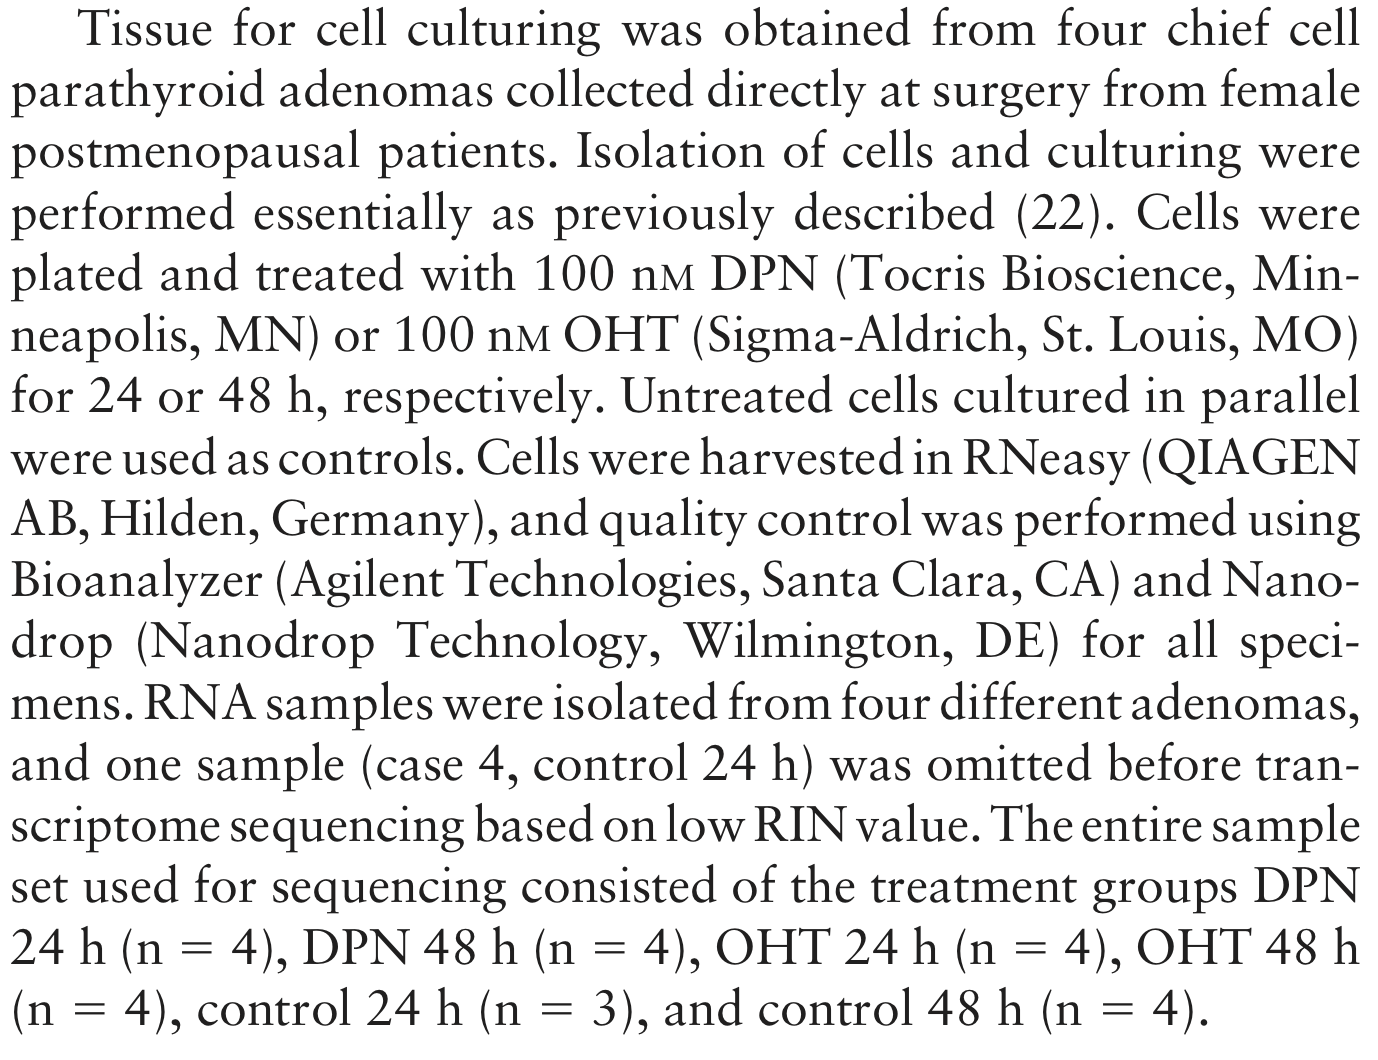
\includegraphics[width=19.14in]{./images_sequencing/expDesign_para} \caption{Figure: A paragraph from the Methods section.}\label{fig:unnamed-chunk-2}
\end{figure}

\end{block}

\begin{block}{Data import and exploration}

We will be importing the dataset using the
\href{https://www.bioconductor.org/packages/release/data/experiment/html/parathyroidSE.html}{parathyroidSE}
data package from \href{https://bioconductor.org/}{Bioconductor}.

\begin{Shaded}
\begin{Highlighting}[]
\ControlFlowTok{if}\NormalTok{ (}\OperatorTok{!}\KeywordTok{requireNamespace}\NormalTok{(}\StringTok{"BiocManager"}\NormalTok{, }\DataTypeTok{quietly =} \OtherTok{TRUE}\NormalTok{))\{}
  \KeywordTok{install.packages}\NormalTok{(}\StringTok{"BiocManager"}\NormalTok{)}
\NormalTok{\}}
\end{Highlighting}
\end{Shaded}

\begin{verbatim}
## Bioconductor version '3.12' is out-of-date; the current release version '3.13'
##   is available with R version '4.1'; see https://bioconductor.org/install
\end{verbatim}

\begin{Shaded}
\begin{Highlighting}[]
\ControlFlowTok{if}\NormalTok{(}\OperatorTok{!}\StringTok{"SummarizedExperiment"} \OperatorTok\StringTok{ }\KeywordTok{installed.packages}\NormalTok{()[,}\DecValTok{1}\NormalTok{])\{}
\NormalTok{  BiocManager}\OperatorTok{::}\KeywordTok{install}\NormalTok{(}\StringTok{"SummarizedExperiment"}\NormalTok{)}
\NormalTok{\} }
\CommentTok{# install package if not installed.}
\ControlFlowTok{if}\NormalTok{(}\OperatorTok{!}\StringTok{"parathyroidSE"} \OperatorTok\StringTok{ }\KeywordTok{installed.packages}\NormalTok{()[,}\DecValTok{1}\NormalTok{]) BiocManager}\OperatorTok{::}\KeywordTok{install}\NormalTok{(}\StringTok{"parathyroidSE"}\NormalTok{)}

\KeywordTok{suppressPackageStartupMessages}\NormalTok{(\{}
  \KeywordTok{library}\NormalTok{(parathyroidSE)}
  \KeywordTok{library}\NormalTok{(SummarizedExperiment)}
\NormalTok{\})}

\CommentTok{# import data}
\KeywordTok{data}\NormalTok{(}\StringTok{"parathyroidGenesSE"}\NormalTok{, }\DataTypeTok{package=}\StringTok{"parathyroidSE"}\NormalTok{)}
\CommentTok{# rename for convenience}
\NormalTok{se1 <-}\StringTok{ }\NormalTok{parathyroidGenesSE}
\KeywordTok{rm}\NormalTok{(parathyroidGenesSE)}

\CommentTok{# three treatments}
\NormalTok{treatment1 <-}\StringTok{ }\KeywordTok{colData}\NormalTok{(se1)}\OperatorTok{$}\NormalTok{treatment}
\KeywordTok{table}\NormalTok{(treatment1)}
\end{Highlighting}
\end{Shaded}

\begin{verbatim}
## treatment1
## Control     DPN     OHT 
##       7      10      10
\end{verbatim}

\begin{Shaded}
\begin{Highlighting}[]
\CommentTok{# two timepoints}
\NormalTok{time1 <-}\StringTok{ }\KeywordTok{colData}\NormalTok{(se1)}\OperatorTok{$}\NormalTok{time}
\KeywordTok{table}\NormalTok{(time1)}
\end{Highlighting}
\end{Shaded}

\begin{verbatim}
## time1
## 24h 48h 
##  13  14
\end{verbatim}

\begin{Shaded}
\begin{Highlighting}[]
\CommentTok{# four donor patients}
\NormalTok{patient1 <-}\StringTok{ }\KeywordTok{colData}\NormalTok{(se1)}\OperatorTok{$}\NormalTok{patient}
\KeywordTok{table}\NormalTok{(patient1)}
\end{Highlighting}
\end{Shaded}

\begin{verbatim}
## patient1
## 1 2 3 4 
## 6 8 6 7
\end{verbatim}

\begin{Shaded}
\begin{Highlighting}[]
\KeywordTok{table}\NormalTok{(patient1, treatment1, time1)}
\end{Highlighting}
\end{Shaded}

\begin{verbatim}
## , , time1 = 24h
## 
##         treatment1
## patient1 Control DPN OHT
##        1       1   1   1
##        2       1   2   2
##        3       1   1   1
##        4       0   1   1
## 
## , , time1 = 48h
## 
##         treatment1
## patient1 Control DPN OHT
##        1       1   1   1
##        2       1   1   1
##        3       1   1   1
##        4       1   2   2
\end{verbatim}

\begin{itemize}
\tightlist
\item
  We observe that the number of samples that we are observing here is
  larger than what is described in the paper. As also described in the
  \href{https://www.bioconductor.org/packages/release/data/experiment/vignettes/parathyroidSE/inst/doc/parathyroidSE.pdf}{parathyroidSE
  vignette}, some samples were spread over multiple sequencing runs
  (i.e., the same sample being sequenced repeatedly) and therefore
  constitute \textbf{technical replication}, rather than biological
  replication.
\item
  We have previously seen that technical replicates can be considered to
  be distributed according to a Poisson distribution. One important
  property of Poisson random variables is that a sum of Poisson random
  variables still follow a Poisson distribution. Indeed, if
  \(X \sim Poi(\mu_X)\) and \(Y \sim Poi(\mu_Y)\), then \$ X + Y = Z
  \sim Poi(\mu\_X + \mu\_Y)\$.
\item
  For this reason, it is often suggested to sum technical replicates
  rather than, for example, averaging, which does not retain the Poisson
  property (try for yourself!). We'll therefore first sum the technical
  replicates.
\end{itemize}

\begin{Shaded}
\begin{Highlighting}[]
\NormalTok{dupExps <-}\StringTok{ }\KeywordTok{as.character}\NormalTok{(}\KeywordTok{colData}\NormalTok{(se1)}\OperatorTok{$}\NormalTok{experiment[}\KeywordTok{duplicated}\NormalTok{(}\KeywordTok{colData}\NormalTok{(se1)}\OperatorTok{$}\NormalTok{experiment)])}
\NormalTok{dupExps}
\end{Highlighting}
\end{Shaded}

\begin{verbatim}
## [1] "SRX140511" "SRX140513" "SRX140523" "SRX140525"
\end{verbatim}

\begin{Shaded}
\begin{Highlighting}[]
\NormalTok{counts <-}\StringTok{ }\KeywordTok{assays}\NormalTok{(se1)}\OperatorTok{$}\NormalTok{counts}
\NormalTok{newCounts <-}\StringTok{ }\NormalTok{counts}
\NormalTok{cd <-}\StringTok{ }\KeywordTok{colData}\NormalTok{(se1)}
\ControlFlowTok{for}\NormalTok{(ss }\ControlFlowTok{in} \DecValTok{1}\OperatorTok{:}\KeywordTok{length}\NormalTok{(dupExps))\{}
  \CommentTok{# check which samples are duplicates}
\NormalTok{  relevantId <-}\StringTok{ }\KeywordTok{which}\NormalTok{(}\KeywordTok{colData}\NormalTok{(se1)}\OperatorTok{$}\NormalTok{experiment }\OperatorTok{==}\StringTok{ }\NormalTok{dupExps[ss])}
  \CommentTok{# sum counts}
\NormalTok{  newCounts[,relevantId[}\DecValTok{1}\NormalTok{]] <-}\StringTok{ }\KeywordTok{rowSums}\NormalTok{(counts[,relevantId])}
  \CommentTok{# keep which columns / rows to remove.}
  \ControlFlowTok{if}\NormalTok{(ss }\OperatorTok{==}\StringTok{ }\DecValTok{1}\NormalTok{)\{}
\NormalTok{    toRemove <-}\StringTok{ }\NormalTok{relevantId[}\DecValTok{2}\NormalTok{]}
\NormalTok{  \} }\ControlFlowTok{else}\NormalTok{ \{}
\NormalTok{    toRemove <-}\StringTok{ }\KeywordTok{c}\NormalTok{(toRemove, relevantId[}\DecValTok{2}\NormalTok{])}
\NormalTok{  \}}
\NormalTok{\}}

\CommentTok{# remove after summing counts (otherwise IDs get mixed up)}
\NormalTok{newCounts <-}\StringTok{ }\NormalTok{newCounts[,}\OperatorTok{-}\NormalTok{toRemove]}
\NormalTok{newCD <-}\StringTok{ }\NormalTok{cd[}\OperatorTok{-}\NormalTok{toRemove,]}

\CommentTok{# Create new SummarizedExperiment}
\NormalTok{se <-}\StringTok{ }\KeywordTok{SummarizedExperiment}\NormalTok{(}\DataTypeTok{assays =} \KeywordTok{list}\NormalTok{(}\StringTok{"counts"}\NormalTok{ =}\StringTok{ }\NormalTok{newCounts),}
                            \DataTypeTok{colData =}\NormalTok{ newCD,}
                            \DataTypeTok{metadata =} \KeywordTok{metadata}\NormalTok{(se1))}

\NormalTok{treatment <-}\StringTok{ }\KeywordTok{colData}\NormalTok{(se)}\OperatorTok{$}\NormalTok{treatment}
\KeywordTok{table}\NormalTok{(treatment)}
\end{Highlighting}
\end{Shaded}

\begin{verbatim}
## treatment
## Control     DPN     OHT 
##       7       8       8
\end{verbatim}

\begin{Shaded}
\begin{Highlighting}[]
\NormalTok{time <-}\StringTok{ }\KeywordTok{colData}\NormalTok{(se)}\OperatorTok{$}\NormalTok{time}
\KeywordTok{table}\NormalTok{(time)}
\end{Highlighting}
\end{Shaded}

\begin{verbatim}
## time
## 24h 48h 
##  11  12
\end{verbatim}

\begin{Shaded}
\begin{Highlighting}[]
\NormalTok{patient <-}\StringTok{ }\KeywordTok{colData}\NormalTok{(se)}\OperatorTok{$}\NormalTok{patient}
\KeywordTok{table}\NormalTok{(patient)}
\end{Highlighting}
\end{Shaded}

\begin{verbatim}
## patient
## 1 2 3 4 
## 6 6 6 5
\end{verbatim}

\begin{Shaded}
\begin{Highlighting}[]
\KeywordTok{table}\NormalTok{(patient, treatment, time) }\CommentTok{# agrees with paper.}
\end{Highlighting}
\end{Shaded}

\begin{verbatim}
## , , time = 24h
## 
##        treatment
## patient Control DPN OHT
##       1       1   1   1
##       2       1   1   1
##       3       1   1   1
##       4       0   1   1
## 
## , , time = 48h
## 
##        treatment
## patient Control DPN OHT
##       1       1   1   1
##       2       1   1   1
##       3       1   1   1
##       4       1   1   1
\end{verbatim}

\begin{itemize}
\tightlist
\item
  After summing the technical replicates and appropriately updating the
  sample information, we again create a \texttt{SummarizedExperiment}
  object, which is essentially a data container that contains all
  relevant information about your experiment. Please see the
  \href{https://bioconductor.org/packages/release/bioc/vignettes/SummarizedExperiment/inst/doc/SummarizedExperiment.html}{vignette}
  for more information on how to use this class.
\item
  By directly matching columns (samples) and rows (genes) to their
  relevant metadata, the \texttt{SummarizedExperiment} class avoids
  mistakes by mis-matching columns and rows with each other (provided
  you haven't mismatched them when you creat the object).
\item
  The \texttt{SummarizedExperiment} class is modular and extendable, and
  extensions exist for example for the analysis of single-cell RNA-seq
  data.
\item
  Due to their convenient organization and widely supported usage within
  Bioconductor, we will typically work with such containers in the
  analysis of RNA-seq data.
\end{itemize}

\end{block}

\begin{block}{Data exploration}

\begin{Shaded}
\begin{Highlighting}[]
\KeywordTok{suppressPackageStartupMessages}\NormalTok{(\{}
  \KeywordTok{library}\NormalTok{(limma)}
  \KeywordTok{library}\NormalTok{(edgeR)}
\NormalTok{\})}

\CommentTok{# library size distribution}
\KeywordTok{hist}\NormalTok{(}\KeywordTok{colSums}\NormalTok{(}\KeywordTok{assays}\NormalTok{(se)}\OperatorTok{$}\NormalTok{counts)}\OperatorTok{/}\FloatTok{1e6}\NormalTok{, }\DataTypeTok{breaks=}\DecValTok{10}\NormalTok{)}
\end{Highlighting}
\end{Shaded}

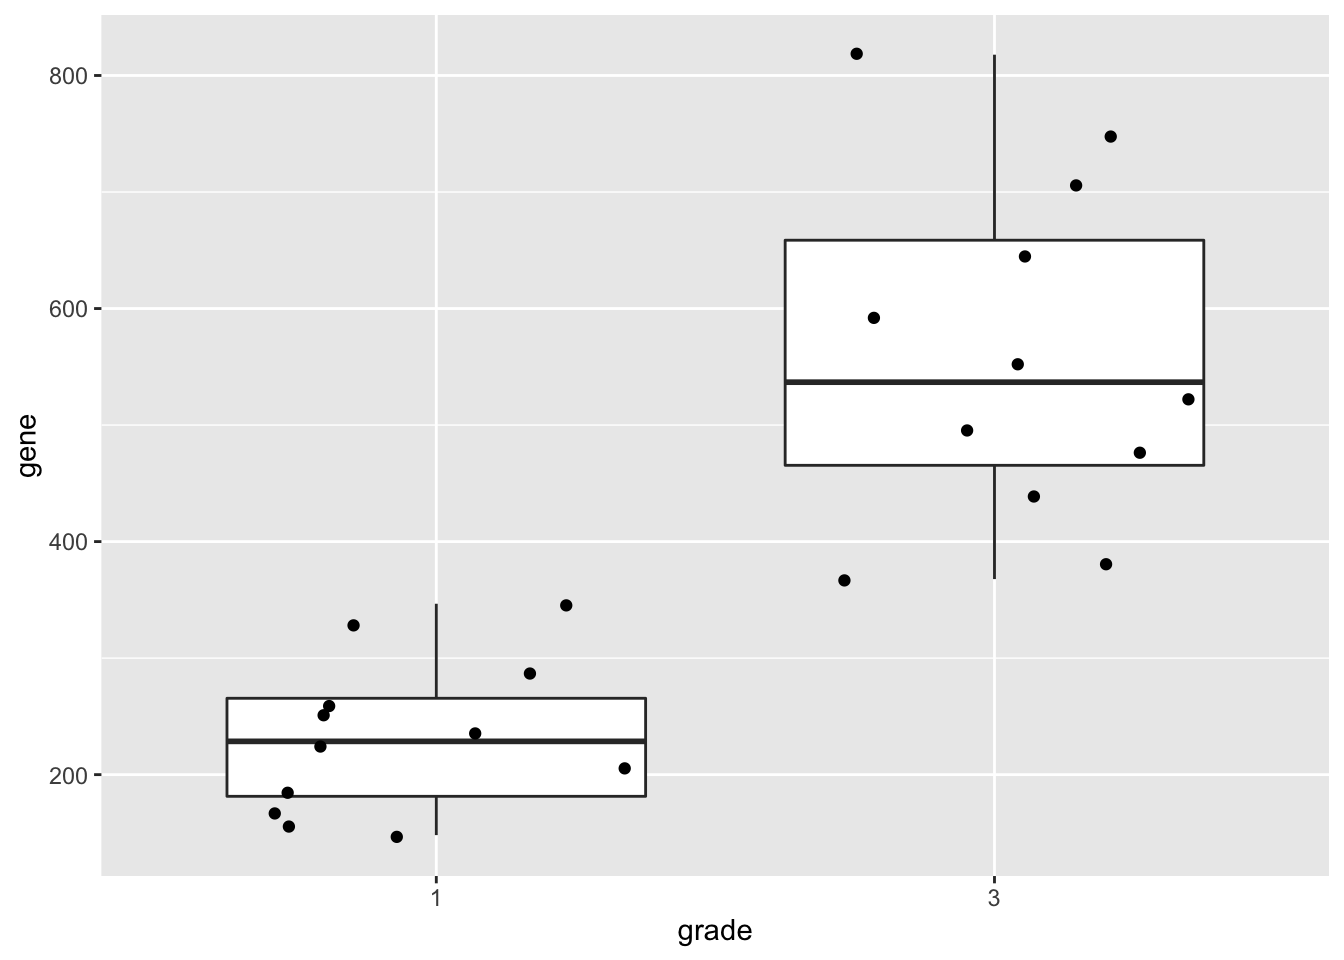
\includegraphics{sequencing_rnaseqIntro_files/figure-beamer/unnamed-chunk-5-1.pdf}

\begin{Shaded}
\begin{Highlighting}[]
\KeywordTok{boxplot}\NormalTok{(}\KeywordTok{colSums}\NormalTok{(}\KeywordTok{assays}\NormalTok{(se)}\OperatorTok{$}\NormalTok{counts)}\OperatorTok{/}\FloatTok{1e6} \OperatorTok{~}\StringTok{ }\NormalTok{treatment)}
\end{Highlighting}
\end{Shaded}

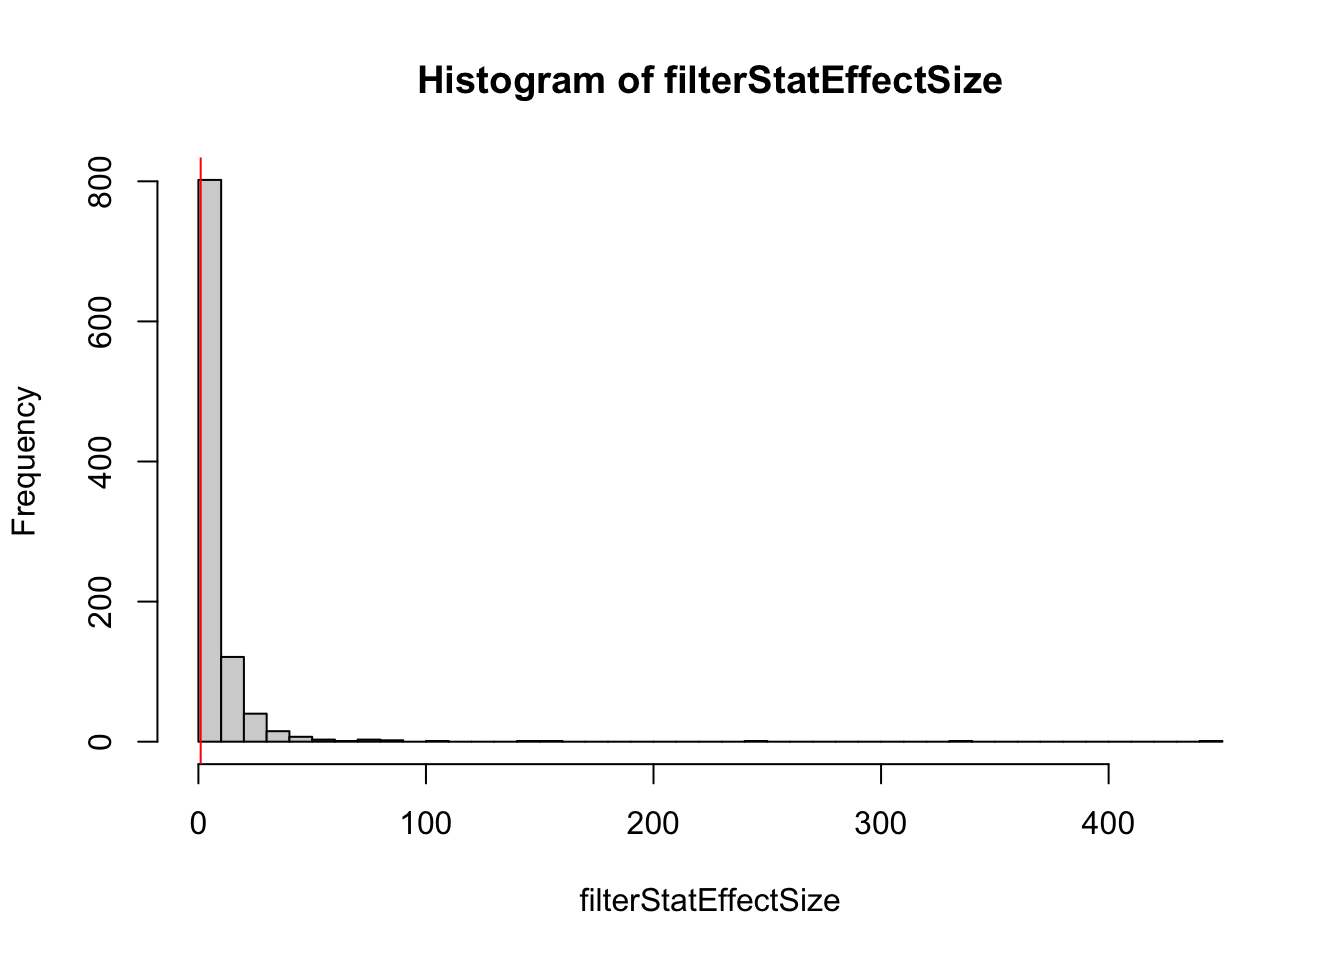
\includegraphics{sequencing_rnaseqIntro_files/figure-beamer/unnamed-chunk-5-2.pdf}

\begin{Shaded}
\begin{Highlighting}[]
\KeywordTok{boxplot}\NormalTok{(}\KeywordTok{colSums}\NormalTok{(}\KeywordTok{assays}\NormalTok{(se)}\OperatorTok{$}\NormalTok{counts)}\OperatorTok{/}\FloatTok{1e6} \OperatorTok{~}\StringTok{ }\NormalTok{time)}
\end{Highlighting}
\end{Shaded}

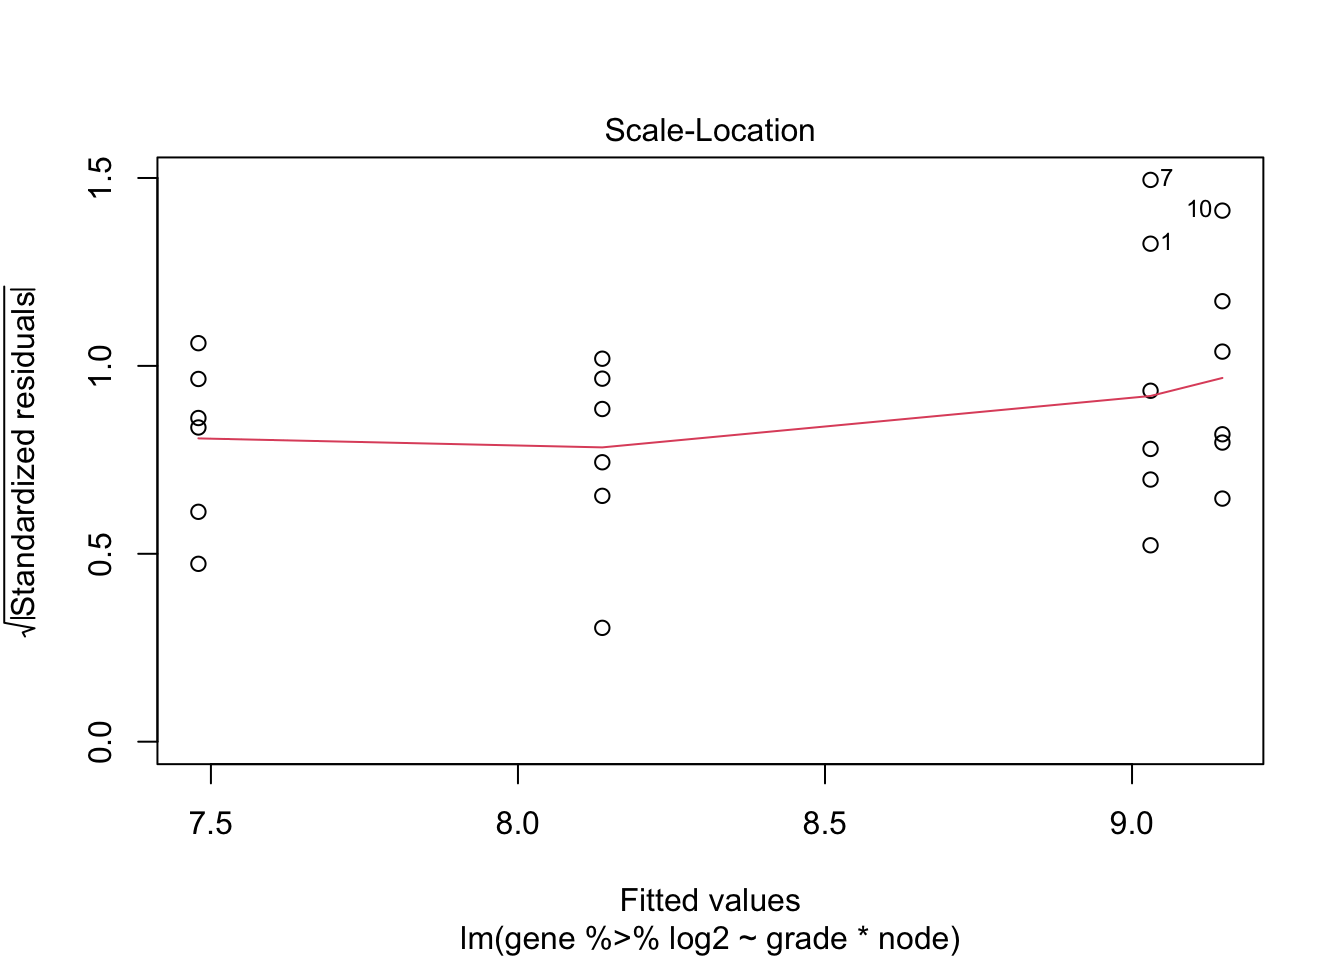
\includegraphics{sequencing_rnaseqIntro_files/figure-beamer/unnamed-chunk-5-3.pdf}

\begin{Shaded}
\begin{Highlighting}[]
\KeywordTok{boxplot}\NormalTok{(}\KeywordTok{colSums}\NormalTok{(}\KeywordTok{assays}\NormalTok{(se)}\OperatorTok{$}\NormalTok{counts)}\OperatorTok{/}\FloatTok{1e6} \OperatorTok{~}\StringTok{ }\NormalTok{patient)}
\end{Highlighting}
\end{Shaded}

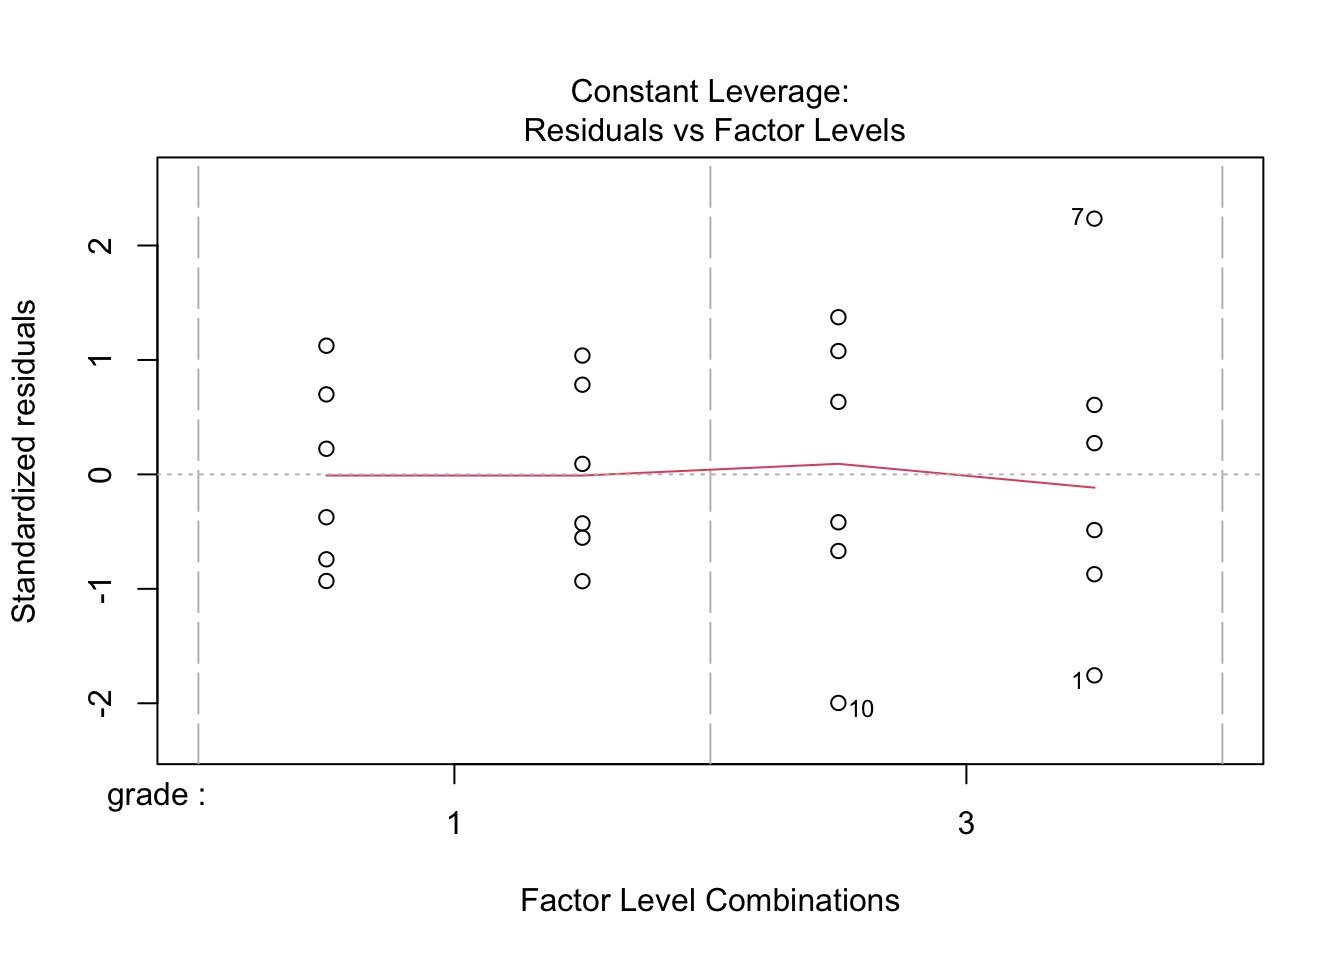
\includegraphics{sequencing_rnaseqIntro_files/figure-beamer/unnamed-chunk-5-4.pdf}

\begin{Shaded}
\begin{Highlighting}[]
\KeywordTok{boxplot}\NormalTok{(}\KeywordTok{colSums}\NormalTok{(}\KeywordTok{assays}\NormalTok{(se)}\OperatorTok{$}\NormalTok{counts)}\OperatorTok{/}\FloatTok{1e6} \OperatorTok{~}\StringTok{ }\KeywordTok{interaction}\NormalTok{(treatment, time))}
\end{Highlighting}
\end{Shaded}

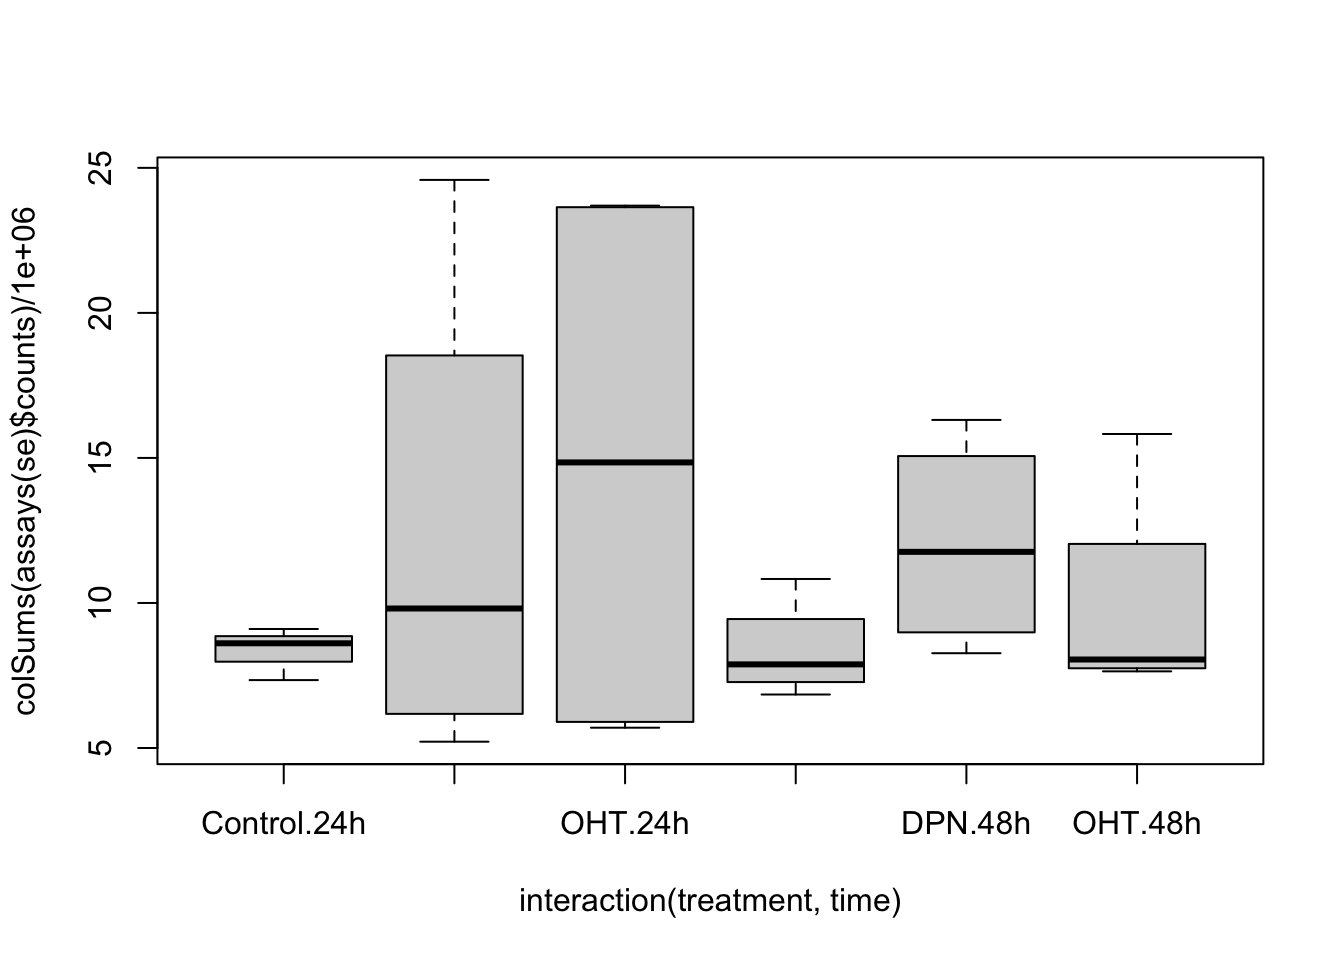
\includegraphics{sequencing_rnaseqIntro_files/figure-beamer/unnamed-chunk-5-5.pdf}

\begin{Shaded}
\begin{Highlighting}[]
\CommentTok{# MDS plot}
\KeywordTok{plotMDS}\NormalTok{(se, }
        \DataTypeTok{labels =}\NormalTok{ treatment, }
        \DataTypeTok{col=}\KeywordTok{as.numeric}\NormalTok{(patient))}
\end{Highlighting}
\end{Shaded}

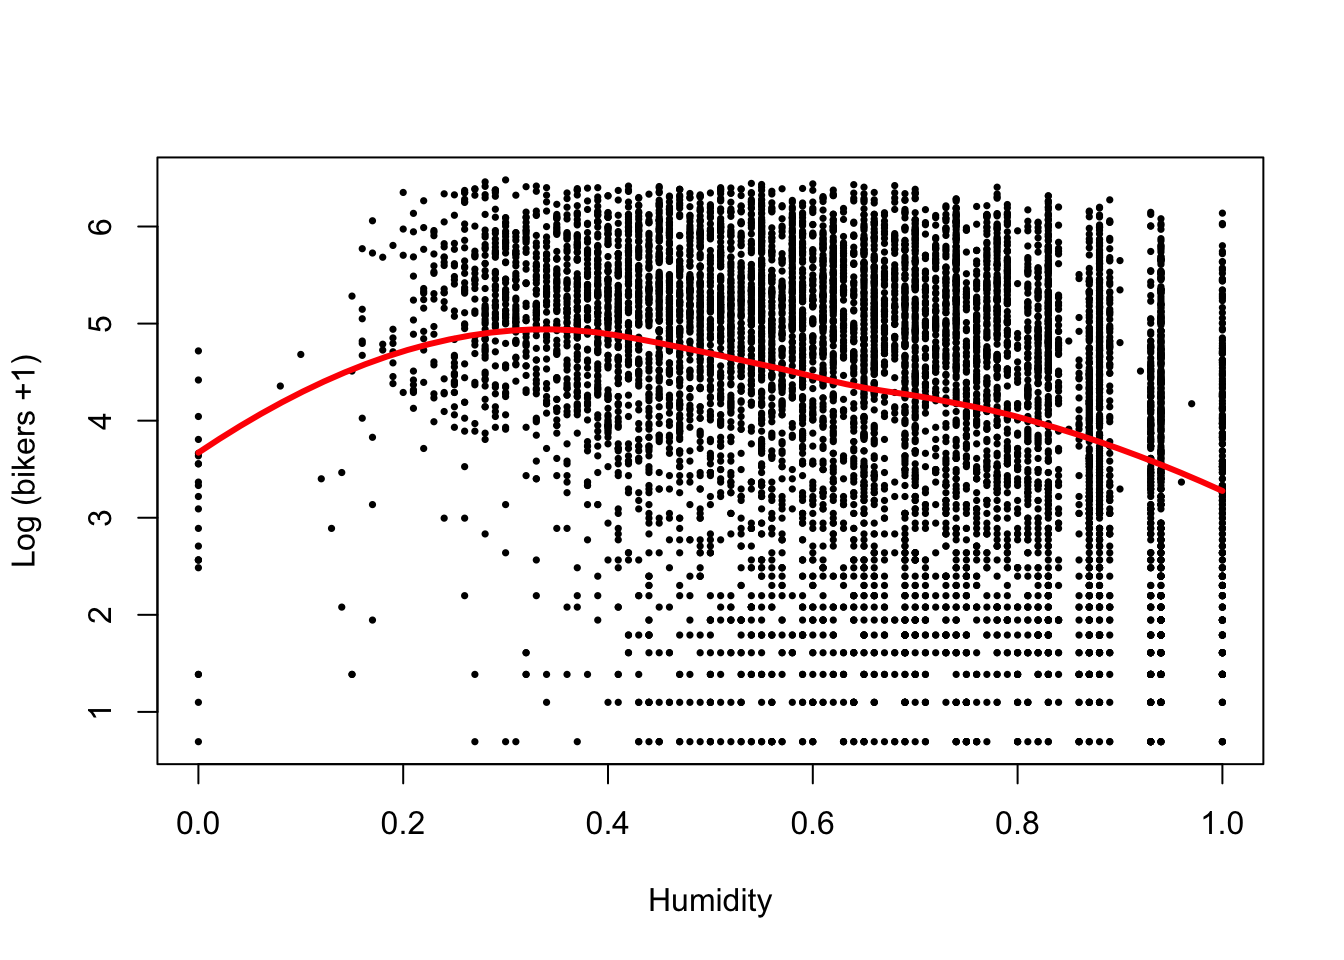
\includegraphics{sequencing_rnaseqIntro_files/figure-beamer/unnamed-chunk-5-6.pdf}

\begin{Shaded}
\begin{Highlighting}[]
\CommentTok{## hard to see influence of experimental factors due to large between-patient variation}
\CommentTok{## we could also make an MDS plot per patient to take a look.}
\ControlFlowTok{for}\NormalTok{(kk }\ControlFlowTok{in} \DecValTok{1}\OperatorTok{:}\DecValTok{4}\NormalTok{)\{}
\NormalTok{  id <-}\StringTok{ }\KeywordTok{which}\NormalTok{(patient }\OperatorTok{==}\StringTok{ }\NormalTok{kk)}
  \KeywordTok{plotMDS}\NormalTok{(se[,id], }
        \DataTypeTok{labels =} \KeywordTok{paste0}\NormalTok{(treatment[id],}\StringTok{"_"}\NormalTok{,time[id]), }
        \DataTypeTok{col=}\KeywordTok{as.numeric}\NormalTok{(time[id]))}
\NormalTok{\}}
\end{Highlighting}
\end{Shaded}

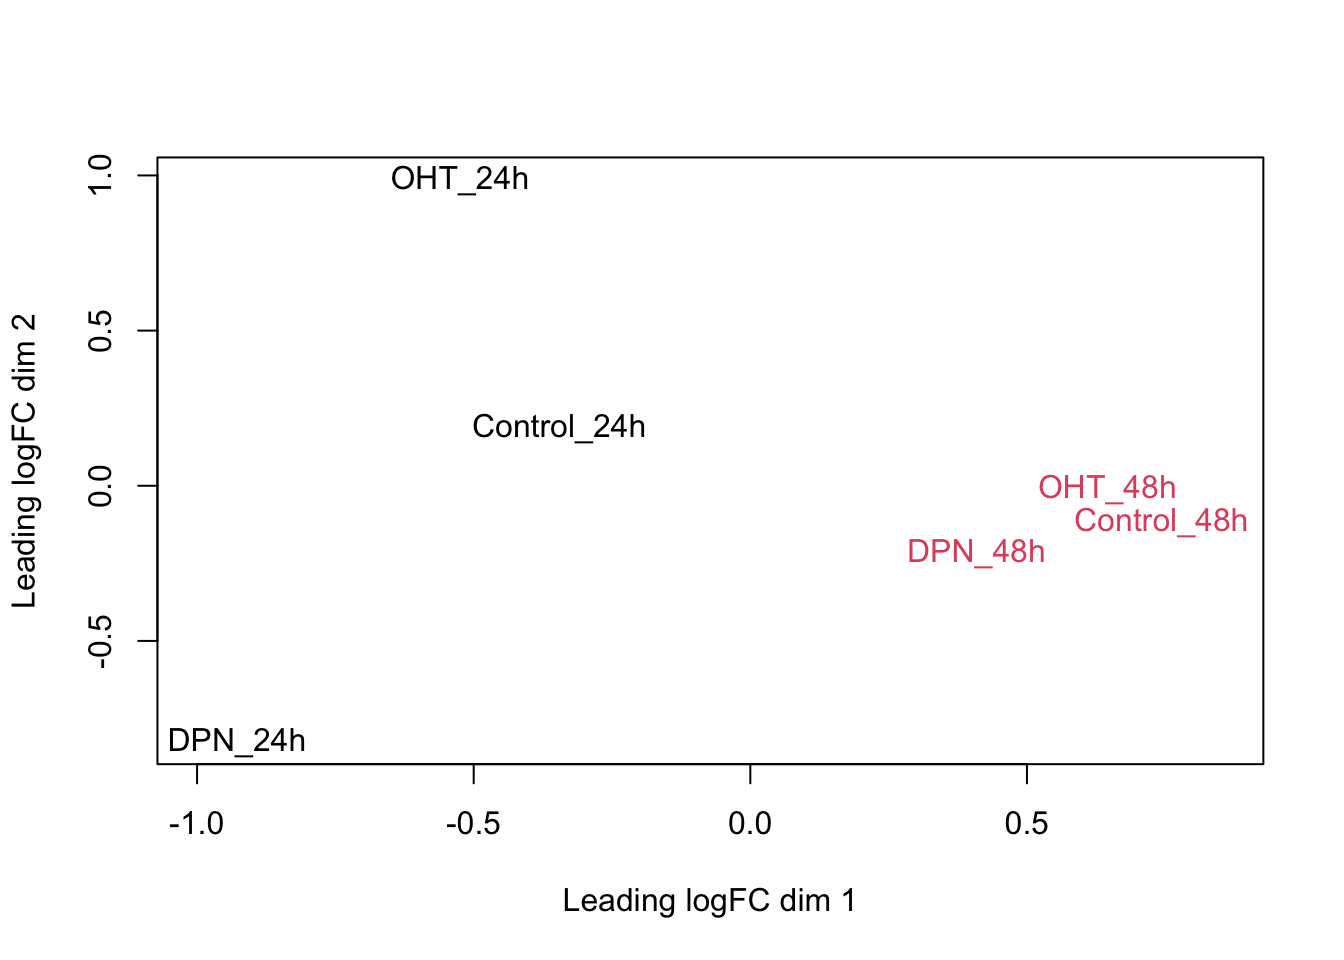
\includegraphics{sequencing_rnaseqIntro_files/figure-beamer/unnamed-chunk-5-7.pdf}
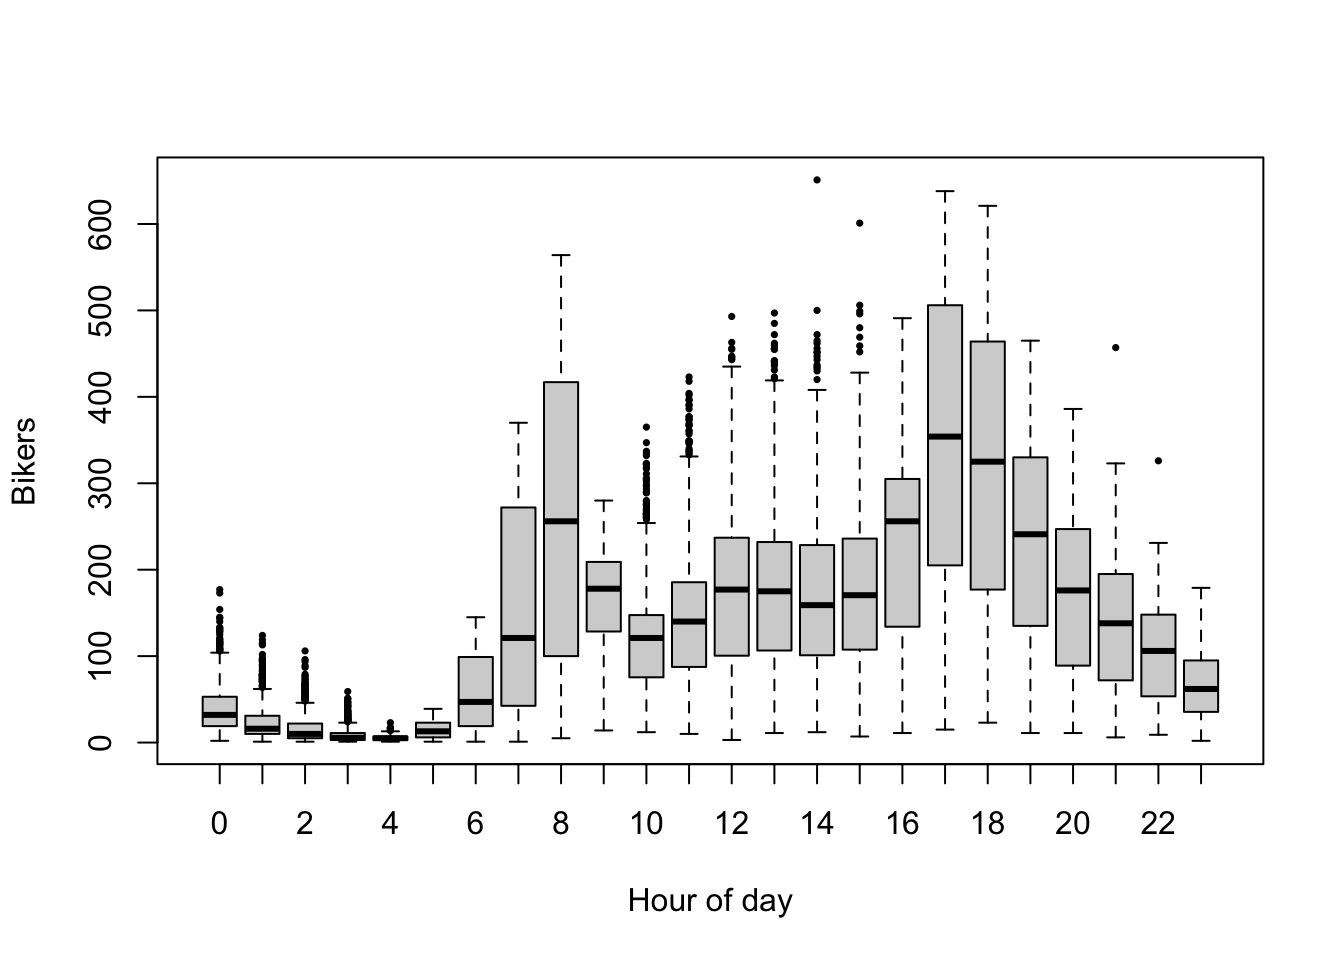
\includegraphics{sequencing_rnaseqIntro_files/figure-beamer/unnamed-chunk-5-8.pdf}
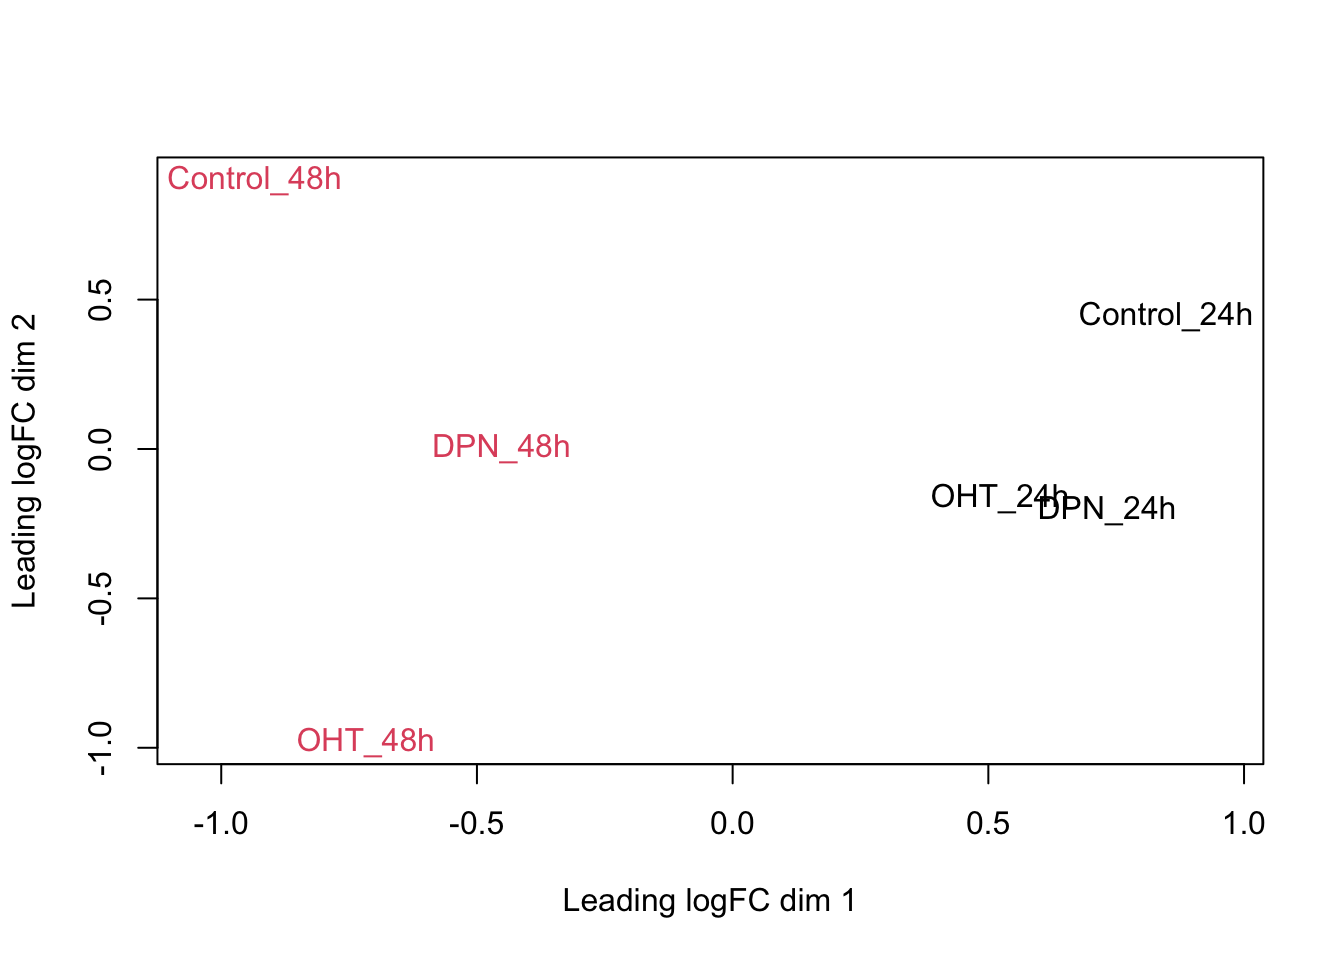
\includegraphics{sequencing_rnaseqIntro_files/figure-beamer/unnamed-chunk-5-9.pdf}
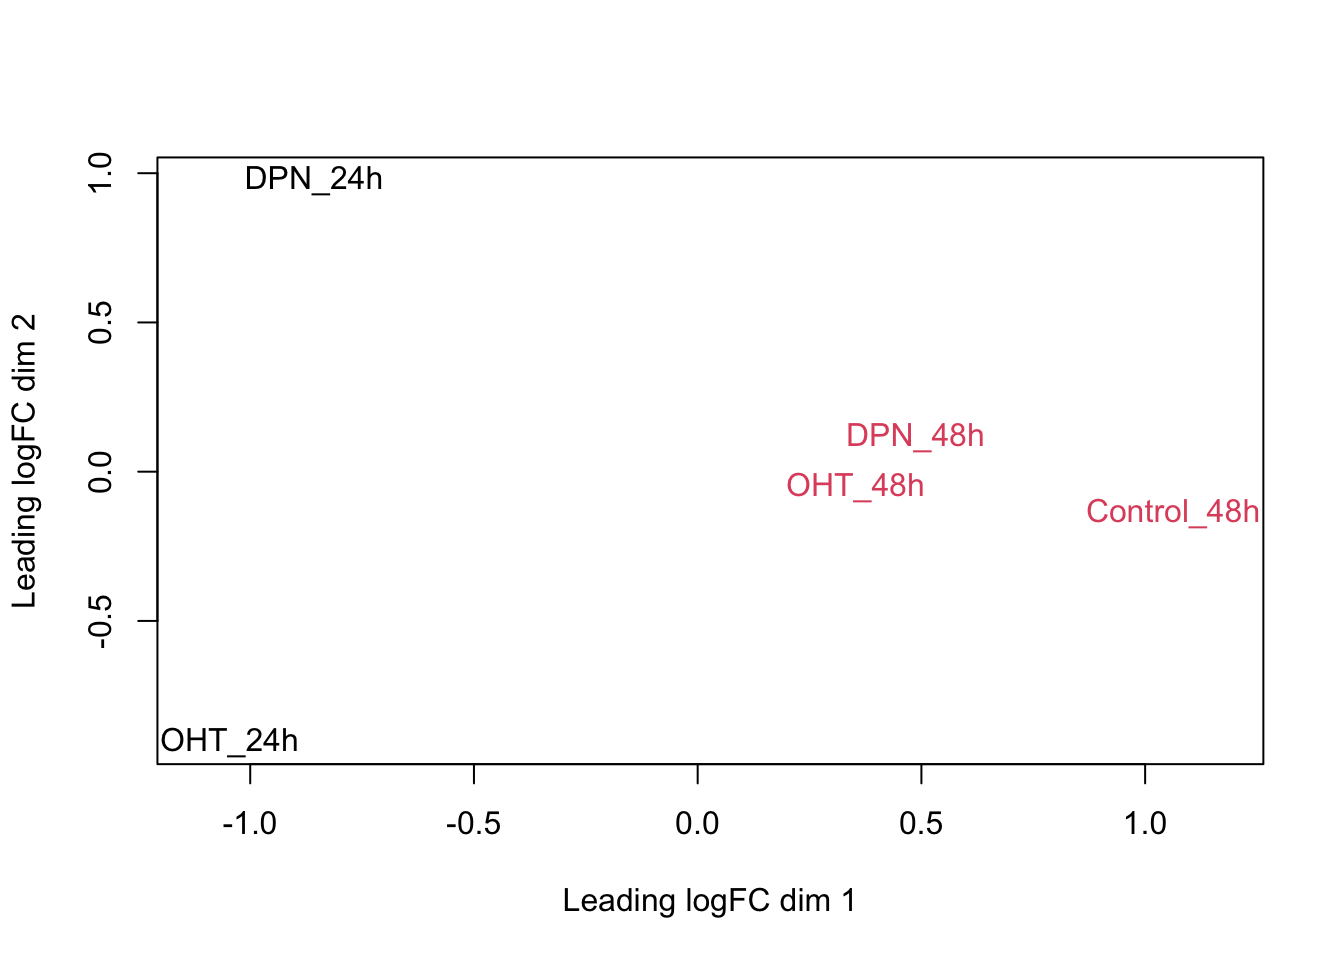
\includegraphics{sequencing_rnaseqIntro_files/figure-beamer/unnamed-chunk-5-10.pdf}

Observations based on MDS plot:

\begin{itemize}
\tightlist
\item
  There is a very large between-patient variability, which is the major
  source of variation in this dataset. The samples from each patient
  cluster together tightly.
\item
  Within patient, time consistently explains more variation than the
  treatments.
\item
  Relative to patients and time, the treatment seems to have a fairly
  small effect.
\end{itemize}

\end{block}

\end{frame}

\begin{frame}[fragile]{Challenge I: Choice of modeling assumptions}
\protect\hypertarget{challenge-i-choice-of-modeling-assumptions}{}

When working with a GLM, as part of the choices of modeling assumptions,
we need to pick an appropriate distribution for the expression counts.
Below we perform some exploratory analyses to investigate.

\begin{Shaded}
\begin{Highlighting}[]
\NormalTok{y <-}\StringTok{ }\KeywordTok{assays}\NormalTok{(se)}\OperatorTok{$}\NormalTok{counts[}\DecValTok{1}\NormalTok{,]}
\KeywordTok{hist}\NormalTok{(y, }\DataTypeTok{breaks =} \DecValTok{40}\NormalTok{,}
     \DataTypeTok{xlab =} \StringTok{"Gene expression"}\NormalTok{,}
     \DataTypeTok{xaxt =} \StringTok{"n"}\NormalTok{, }\DataTypeTok{yaxt =} \StringTok{"n"}\NormalTok{,}
     \DataTypeTok{main =} \StringTok{"Data for the first gene"}\NormalTok{)}
\KeywordTok{axis}\NormalTok{(}\DecValTok{1}\NormalTok{, }\DataTypeTok{at =} \KeywordTok{seq}\NormalTok{(}\DecValTok{200}\NormalTok{, }\DecValTok{1200}\NormalTok{, }\DataTypeTok{by=}\DecValTok{200}\NormalTok{))}
\KeywordTok{axis}\NormalTok{(}\DecValTok{2}\NormalTok{, }\DataTypeTok{at =} \DecValTok{0}\OperatorTok{:}\DecValTok{3}\NormalTok{)}
\end{Highlighting}
\end{Shaded}

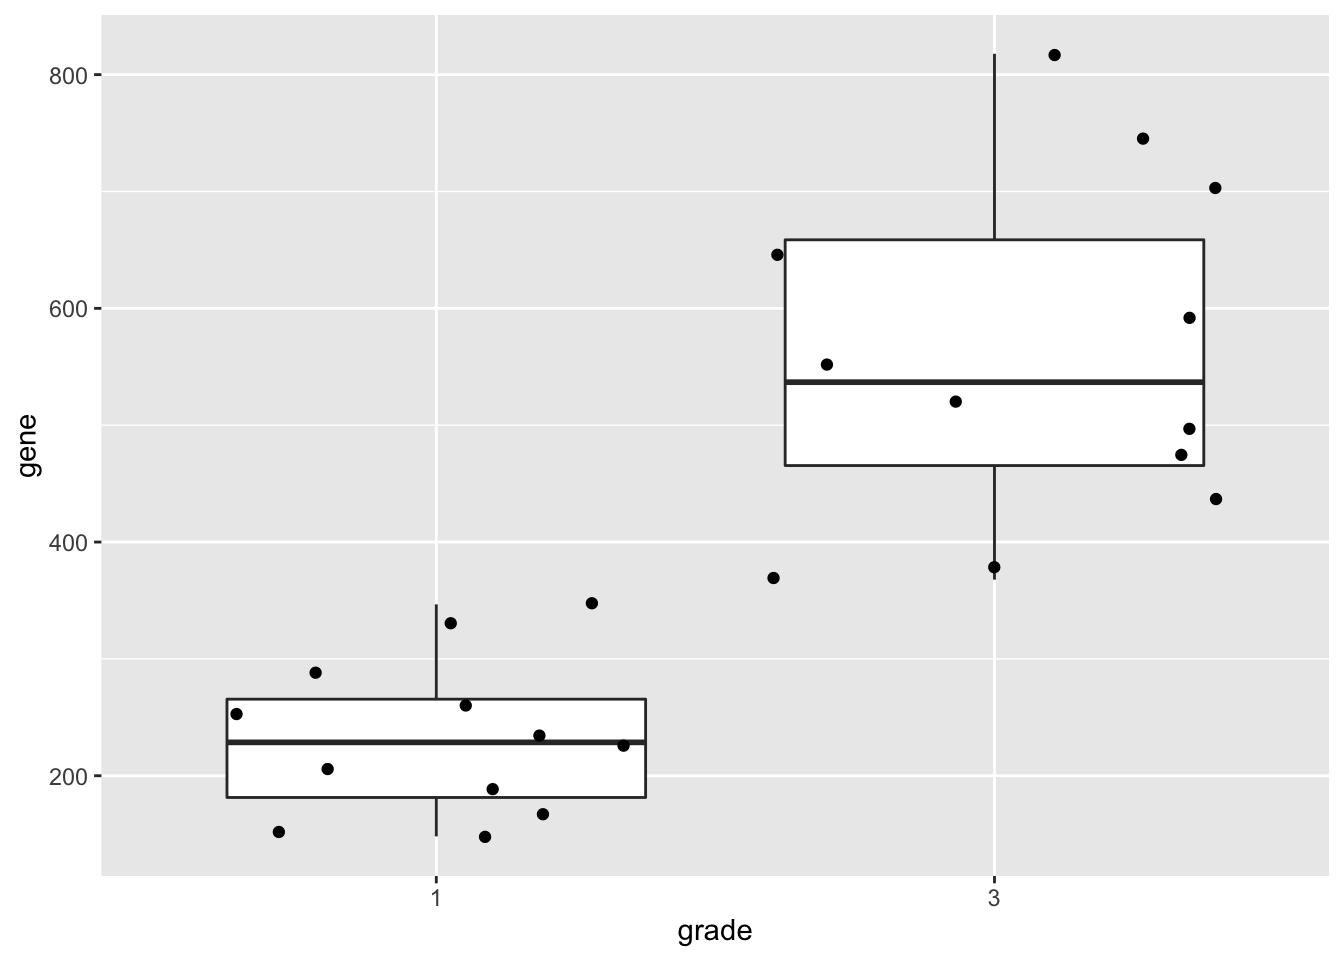
\includegraphics{sequencing_rnaseqIntro_files/figure-beamer/unnamed-chunk-7-1.pdf}

\begin{Shaded}
\begin{Highlighting}[]
\CommentTok{# Mean-variance trend within each experimental condition}
\NormalTok{cont24ID <-}\StringTok{ }\KeywordTok{which}\NormalTok{(treatment }\OperatorTok{==}\StringTok{ "Control"} \OperatorTok{&}\StringTok{ }\NormalTok{time }\OperatorTok{==}\StringTok{ "24h"}\NormalTok{)}
\NormalTok{DPN24ID <-}\StringTok{ }\KeywordTok{which}\NormalTok{(treatment }\OperatorTok{==}\StringTok{ "DPN"} \OperatorTok{&}\StringTok{ }\NormalTok{time }\OperatorTok{==}\StringTok{ "24h"}\NormalTok{)}
\NormalTok{OHT24ID <-}\StringTok{ }\KeywordTok{which}\NormalTok{(treatment }\OperatorTok{==}\StringTok{ "OHT"} \OperatorTok{&}\StringTok{ }\NormalTok{time }\OperatorTok{==}\StringTok{ "24h"}\NormalTok{)}
\NormalTok{cont48ID <-}\StringTok{ }\KeywordTok{which}\NormalTok{(treatment }\OperatorTok{==}\StringTok{ "Control"} \OperatorTok{&}\StringTok{ }\NormalTok{time }\OperatorTok{==}\StringTok{ "48h"}\NormalTok{)}
\NormalTok{DPN48ID <-}\StringTok{ }\KeywordTok{which}\NormalTok{(treatment }\OperatorTok{==}\StringTok{ "DPN"} \OperatorTok{&}\StringTok{ }\NormalTok{time }\OperatorTok{==}\StringTok{ "48h"}\NormalTok{)}
\NormalTok{OHT48ID <-}\StringTok{ }\KeywordTok{which}\NormalTok{(treatment }\OperatorTok{==}\StringTok{ "OHT"} \OperatorTok{&}\StringTok{ }\NormalTok{time }\OperatorTok{==}\StringTok{ "48h"}\NormalTok{)}
\NormalTok{idList <-}\StringTok{ }\KeywordTok{list}\NormalTok{(cont24ID, DPN24ID, OHT24ID, }
\NormalTok{               cont48ID, DPN48ID, OHT48ID)}
\KeywordTok{names}\NormalTok{(idList) <-}\StringTok{ }\KeywordTok{paste0}\NormalTok{(}\KeywordTok{rep}\NormalTok{(}\KeywordTok{levels}\NormalTok{(treatment),}\DecValTok{2}\NormalTok{), }\KeywordTok{rep}\NormalTok{(}\KeywordTok{levels}\NormalTok{(time), }\DataTypeTok{each=}\DecValTok{3}\NormalTok{))}

\KeywordTok{par}\NormalTok{(}\DataTypeTok{mfrow=}\KeywordTok{c}\NormalTok{(}\DecValTok{3}\NormalTok{,}\DecValTok{2}\NormalTok{), }\DataTypeTok{mar=}\KeywordTok{c}\NormalTok{(}\DecValTok{2}\NormalTok{,}\DecValTok{2}\NormalTok{,}\DecValTok{2}\NormalTok{,}\DecValTok{1}\NormalTok{))}
\ControlFlowTok{for}\NormalTok{(kk }\ControlFlowTok{in} \DecValTok{1}\OperatorTok{:}\KeywordTok{length}\NormalTok{(idList))\{}
  \CommentTok{# extract counts for each condition}
\NormalTok{  curCounts <-}\StringTok{ }\KeywordTok{assays}\NormalTok{(se)}\OperatorTok{$}\NormalTok{counts[,idList[[kk]]]}
  \KeywordTok{plot}\NormalTok{(}\DataTypeTok{x =} \KeywordTok{rowMeans}\NormalTok{(curCounts)}\OperatorTok{+}\DecValTok{1}\NormalTok{,}
       \DataTypeTok{y =} \KeywordTok{rowVars}\NormalTok{(curCounts)}\OperatorTok{+}\DecValTok{1}\NormalTok{,}
       \DataTypeTok{pch =} \DecValTok{16}\NormalTok{, }\DataTypeTok{cex=}\DecValTok{1}\OperatorTok{/}\DecValTok{2}\NormalTok{,}
       \DataTypeTok{xlab =} \StringTok{"Mean"}\NormalTok{, }\DataTypeTok{ylab=}\StringTok{"Variance"}\NormalTok{,}
       \DataTypeTok{log=}\StringTok{"xy"}\NormalTok{)}
  \KeywordTok{abline}\NormalTok{(}\DecValTok{0}\NormalTok{,}\DecValTok{1}\NormalTok{, }\DataTypeTok{col=}\StringTok{"red"}\NormalTok{)}
  
  \KeywordTok{smoothScatter}\NormalTok{(}\DataTypeTok{x =} \KeywordTok{log1p}\NormalTok{(}\KeywordTok{rowMeans}\NormalTok{(curCounts)),}
       \DataTypeTok{y =} \KeywordTok{log1p}\NormalTok{(}\KeywordTok{rowVars}\NormalTok{(curCounts)),}
       \DataTypeTok{pch =} \DecValTok{16}\NormalTok{, }\DataTypeTok{cex=}\DecValTok{1}\OperatorTok{/}\DecValTok{2}\NormalTok{,}
       \DataTypeTok{xlab =} \StringTok{"Mean"}\NormalTok{, }\DataTypeTok{ylab=}\StringTok{"Variance"}\NormalTok{)}
  \KeywordTok{abline}\NormalTok{(}\DecValTok{0}\NormalTok{,}\DecValTok{1}\NormalTok{, }\DataTypeTok{col=}\StringTok{"red"}\NormalTok{)}
\NormalTok{\}}
\end{Highlighting}
\end{Shaded}

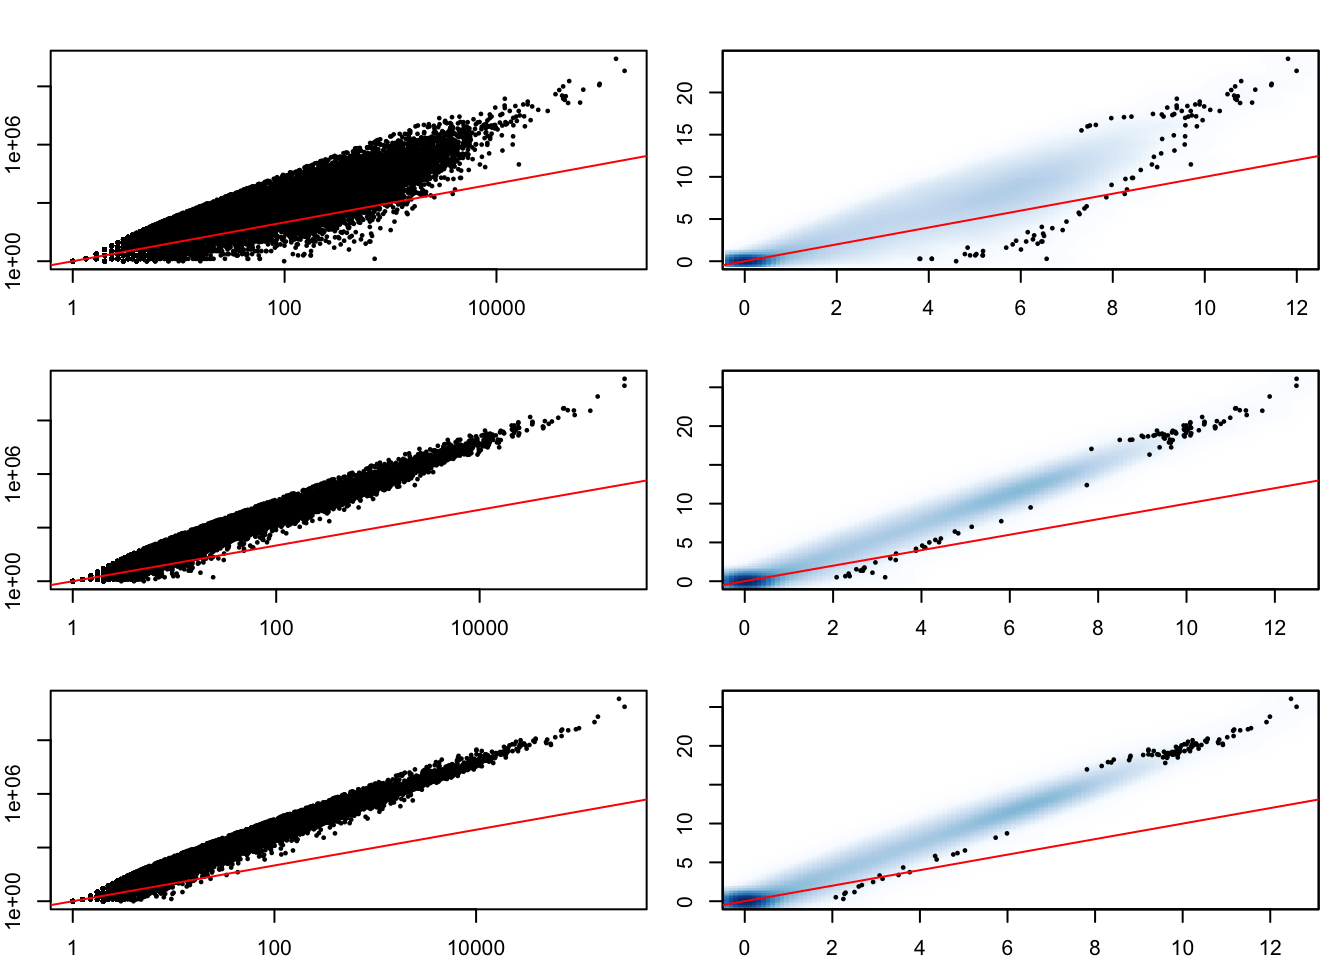
\includegraphics{sequencing_rnaseqIntro_files/figure-beamer/unnamed-chunk-7-2.pdf}
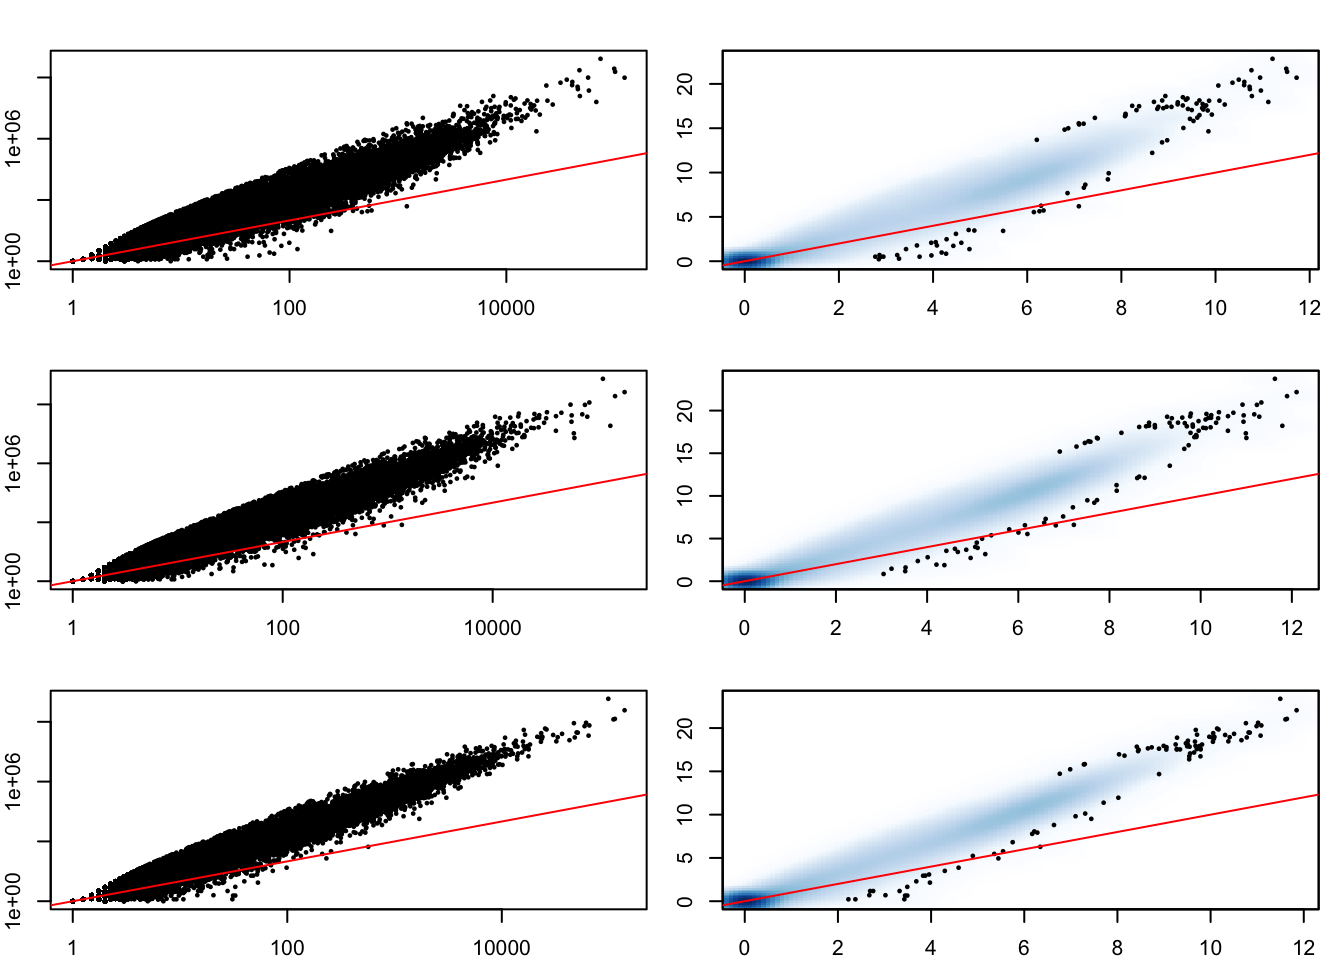
\includegraphics{sequencing_rnaseqIntro_files/figure-beamer/unnamed-chunk-7-3.pdf}

\begin{itemize}
\tightlist
\item
  Having data on thousands of genes provides the opportunity to
  empirically assess the mean-variance relationship.
\item
  It is clear that the data is overdispersed with respect to the Poisson
  distribution. There also seems to be a quadratic trend of the variance
  as a function of the mean. This has motivated the \textbf{negative
  binomial distribution as the most popular choice to model (bulk)
  RNA-seq gene expression data}.
\end{itemize}

\end{frame}

\begin{frame}[fragile]

\begin{itemize}
\tightlist
\item
  The negative binomial distribution is also referred to as the
  Gamma-Poisson distribution as it can be formulated as such. Indeed, if
  \[
   \lambda \sim \Gamma(\alpha, \beta) \\
   Y | \lambda \sim Poi(\lambda),
   \] then this is equivalent to
  \[ Y \sim NB(\mu = \alpha / \beta, \phi = 1/\alpha). \]
\item
  This can be shown analytically, but is considered out of the scope of
  this course. Below, we show it empirically using simulation.
\item
  This theoretical result has got some practical consequences. The
  Gamma-Poisson formulation makes it clear why we can sum technical
  replicates as the sum of Poisson random variables is again a Poisson
  random variable.
\item
  The Poisson statement can thus be considered as capturing technical
  variation, while the Gamma statement can be considered to capture
  biological variation, i.e., variation in the expression mean across
  biological replicates.
\end{itemize}

\begin{Shaded}
\begin{Highlighting}[]
\NormalTok{alpha <-}\StringTok{ }\DecValTok{20}
\NormalTok{beta <-}\StringTok{ }\DecValTok{10}
\NormalTok{lambda <-}\StringTok{ }\KeywordTok{rgamma}\NormalTok{(}\DataTypeTok{n =} \FloatTok{1e5}\NormalTok{, }\DataTypeTok{shape =}\NormalTok{ alpha, }\DataTypeTok{rate =}\NormalTok{ beta)}
\NormalTok{y1 <-}\StringTok{ }\KeywordTok{rpois}\NormalTok{(}\DataTypeTok{n =} \FloatTok{1e5}\NormalTok{, }\DataTypeTok{lambda =}\NormalTok{ lambda)}

\CommentTok{# note phi = 1 / size}
\NormalTok{y2 <-}\StringTok{ }\KeywordTok{rnbinom}\NormalTok{(}\DataTypeTok{n=}\FloatTok{1e5}\NormalTok{, }\DataTypeTok{mu=}\NormalTok{alpha }\OperatorTok{/}\StringTok{ }\NormalTok{(beta), }\DataTypeTok{size=}\NormalTok{alpha)}


\KeywordTok{plot}\NormalTok{(}\KeywordTok{density}\NormalTok{(y1))}
\KeywordTok{lines}\NormalTok{(}\KeywordTok{density}\NormalTok{(y2), }\DataTypeTok{col=}\StringTok{"steelblue"}\NormalTok{)}
\end{Highlighting}
\end{Shaded}

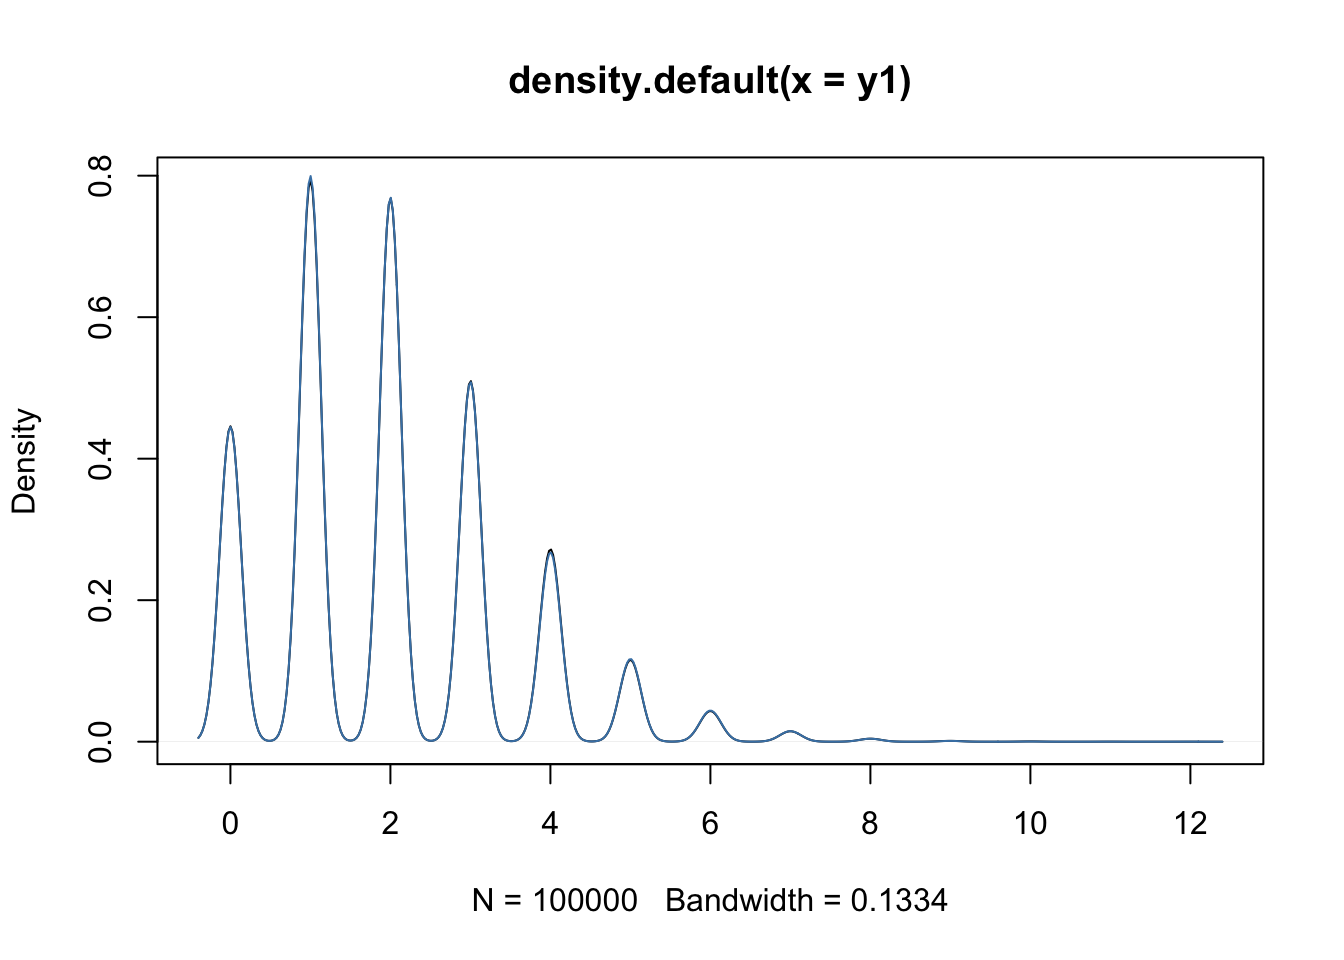
\includegraphics{sequencing_rnaseqIntro_files/figure-beamer/unnamed-chunk-9-1.pdf}

\end{frame}

\begin{frame}{Challenge II: Normalization}
\protect\hypertarget{challenge-ii-normalization}{}

Normalization is necessary to correct for several sources of technical
variation:

\begin{itemize}
\tightlist
\item
  \textbf{Differences in sequencing depth} between samples. Some samples
  get sequenced deeper in the sense that they consist of more (mapped)
  reads and therefore can be considered to contain a higher amount of
  information, which we should be taking into account. In addition, if a
  sample is sequenced deeper, it is natural that the counts for each
  gene will be higher, jeopardizing a direct comparison of the
  expression counts.
\item
  \textbf{Differences in RNA population composition} between samples.
  Suppose that two samples have been sequenced to the exact same depth.
  One sample is contaminated and has a very high concentration of the
  contaminant cDNA being sequenced, but otherwise the two samples are
  identical. Since the contaminant will be taking up a significant
  proportion of the reads being sequenced, the counts will not be
  directly comparable between the samples. Hence, we may also want to
  correct for differences in the composition of the RNA population of
  the samples.
\item
  \textbf{Other technical variation} such as sample-specific GC-content
  or transcript length effects may also be accounted for.
\end{itemize}

\end{frame}

\begin{frame}[fragile]

Let's take a look at how comparable different replicates are in the
Control condition at 48h in our dataset. We will investigate this using
MD-plots (mean-difference plots as introduced by
\href{https://www.jstor.org/stable/24307038}{Dudoit \emph{et al.}
(2002)}), also sometimes referred to as MA-plots.

\begin{Shaded}
\begin{Highlighting}[]
\NormalTok{cont48ID }\CommentTok{# relevant samples}
\end{Highlighting}
\end{Shaded}

\begin{verbatim}
## [1]  2  8 14 19
\end{verbatim}

\begin{Shaded}
\begin{Highlighting}[]
\KeywordTok{colSums}\NormalTok{(}\KeywordTok{assays}\NormalTok{(se)}\OperatorTok{$}\NormalTok{counts[,cont48ID]) }\OperatorTok{/}\StringTok{ }\FloatTok{1e6}
\end{Highlighting}
\end{Shaded}

\begin{verbatim}
## [1] 10.827109  6.844144  8.064268  7.701432
\end{verbatim}

\begin{Shaded}
\begin{Highlighting}[]
\NormalTok{combs <-}\StringTok{ }\KeywordTok{combn}\NormalTok{(cont48ID, }\DataTypeTok{m=}\DecValTok{2}\NormalTok{) }\CommentTok{#pairwise combinations between samples}

\KeywordTok{par}\NormalTok{(}\DataTypeTok{mfrow=}\KeywordTok{c}\NormalTok{(}\DecValTok{3}\NormalTok{,}\DecValTok{2}\NormalTok{), }\DataTypeTok{mar=}\KeywordTok{c}\NormalTok{(}\DecValTok{4}\NormalTok{,}\DecValTok{4}\NormalTok{,}\DecValTok{2}\NormalTok{,}\DecValTok{1}\NormalTok{))}
\ControlFlowTok{for}\NormalTok{(cc }\ControlFlowTok{in} \DecValTok{1}\OperatorTok{:}\KeywordTok{ncol}\NormalTok{(combs))\{}
\NormalTok{  curSamples <-}\StringTok{ }\NormalTok{combs[,cc]}
\NormalTok{  M <-}\StringTok{ }\KeywordTok{rowMeans}\NormalTok{(}\KeywordTok{assays}\NormalTok{(se)}\OperatorTok{$}\NormalTok{counts[,curSamples])}
\NormalTok{  D <-}\StringTok{ }\KeywordTok{assays}\NormalTok{(se)}\OperatorTok{$}\NormalTok{counts[,curSamples[}\DecValTok{2}\NormalTok{]] }\OperatorTok{/}\StringTok{ }\KeywordTok{assays}\NormalTok{(se)}\OperatorTok{$}\NormalTok{counts[,curSamples[}\DecValTok{1}\NormalTok{]]}
  \KeywordTok{plot}\NormalTok{(}\DataTypeTok{x =} \KeywordTok{log}\NormalTok{(M), }\DataTypeTok{y =} \KeywordTok{log2}\NormalTok{(D),}
       \DataTypeTok{pch =} \DecValTok{16}\NormalTok{, }\DataTypeTok{cex=}\DecValTok{1}\OperatorTok{/}\DecValTok{3}\NormalTok{,}
       \DataTypeTok{main =} \KeywordTok{paste0}\NormalTok{(}\StringTok{"Sample "}\NormalTok{, curSamples[}\DecValTok{2}\NormalTok{], }\StringTok{" vs sample "}\NormalTok{, curSamples[}\DecValTok{1}\NormalTok{]),}
       \DataTypeTok{xlab =} \StringTok{"Log mean"}\NormalTok{, }\DataTypeTok{ylab =} \StringTok{"Log2 fold-change"}\NormalTok{,}
       \DataTypeTok{bty =} \StringTok{'l'}\NormalTok{)}
  \KeywordTok{abline}\NormalTok{(}\DataTypeTok{h =} \DecValTok{0}\NormalTok{, }\DataTypeTok{col=}\StringTok{"orange"}\NormalTok{, }\DataTypeTok{lwd=}\DecValTok{2}\NormalTok{)}
\NormalTok{\}}
\end{Highlighting}
\end{Shaded}

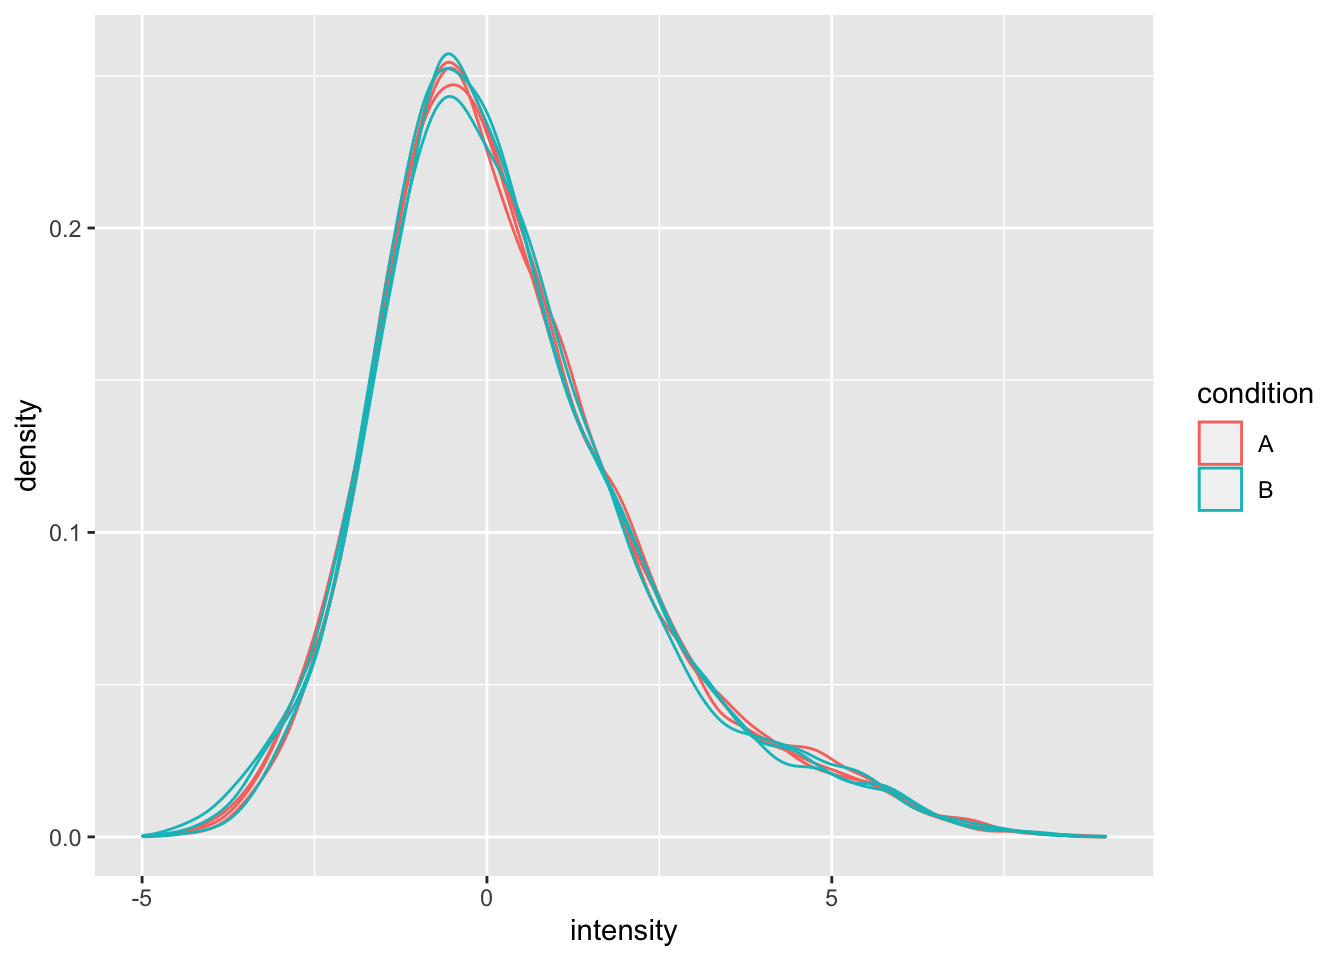
\includegraphics{sequencing_rnaseqIntro_files/figure-beamer/unnamed-chunk-10-1.pdf}

\begin{itemize}
\tightlist
\item
  We see clear bias for some pairwise comparisons. For example, in the
  first plot comparing sample 8 versus sample 2, the log fold-changes
  are biased downwards. This means that, on average, a gene is lower
  expressed in sample 8 versus sample 2. Looking at the library sizes,
  we can indeed see that the library size for sample 2 is about
  \(11 \times 10^6\) while it is only about \(7 \times 10^6\) for sample
  8! This is clear library size effect that we should take into account.
\end{itemize}

\begin{block}{Count scaling versus GLM offsets}

\begin{itemize}
\tightlist
\item
  We have previously discussed count scaling transformations such as CPM
  and TPM as normalization methods that directly scale counts. However,
  these transformations ignore inherent information such as the
  sequencing depth. A measured gene expression of zero in a sample where
  only 1000 reads are sequenced is very different from a sample where 10
  million reads are sequenced.
\item
  A more appropriate and natural way when working with GLMs is through
  the use of \textbf{offsets}. The general use of an offset is to
  account for the `effort' performed in order to gather that observation
  of the response variable. Two examples:

  \begin{enumerate}
  \tightlist
  \item
    A biologist studying whale migration has one fixed spot where, in
    the migration season, she counts migrating whales day after day,
    over several years. For each day she records the number of spotted
    whales. Of course, the time spent whale-watching may differ from day
    to day and it is natural that you are more likely to spot more
    whales if you spend more time looking for them. The time spent
    spotting whales can then be used as an offset.
  \item
    In our case, a sample being sequenced deeper contains more
    information, i.e., more `effort' has been performed, as compared to
    a sample being sequenced relatively shallow. We have more confidence
    of a count from a deeply sequenced sample than from a shallowly
    sequenced sample. We can therefore use the sequencing depth
    \(N_i = \sum_g Y_{gi}\) as off set in the model.
  \end{enumerate}
\item
  Adding an offset to the model is different from adding a new variable
  to the model. For each new variable we add, we will estimate its
  average effect \(\beta\) on the response variable. When adding an
  offset, however, we are implicitly assuming that \(\beta=1\).
\item
  Offsets are typically added on the scale of the linear predictor.
  Suppose we have a gene \(g\) and sample \(i\) specific offset
  \(O_{ij}\), then we can define a negative binomial GLM including the
  offset as \[
    \left\{
    \begin{array}{ccc}
    Y_{gi} & \sim & NB(\mu_{gi}, \phi_g) \\
    \log \mu_{gi} & = & \eta_{gi} \\
    \eta_{gi} & = & \mathbf{X}^T_i \beta_g + \log(O_{gi}). \\
    \end{array}
    \right.
    \]
\end{itemize}

\end{block}

\begin{block}{How to normalize?}

Many approaches are available for normalizing RNA-seq data. Most methods
basically calculate an offset that is added to the GLM used to model
gene expression. One notable method, full-quantile normalization, does
not calculate an offset.

\begin{block}{TMM method (default of \texttt{edgeR})}

The trimmed mean of M-values (TMM) method introduced by
\href{https://genomebiology.biomedcentral.com/articles/10.1186/gb-2010-11-3-r25}{Robinson
\& Oshlack (2010)} is a global-scaling normalization procedure. As the
name suggests, it is based on a trimmed mean of fold-changes
(\(M\)-values) as the scaling factor. A trimmed mean is an average after
removing a set of ``extreme'' values. Specifically, TMM calculates a
normalization factor \(F_i^{(r)}\) across genes \(g\) for each sample
\(i\) as compared to a reference sample \(r\), \[
\log_2(F_i^{(r)}) = \frac{\sum_{g \in {\cal G}^*} w_{gi}^r M_{gi}^r}{\sum_{g \in {\cal G}^*} w_{gi}^r},
\] where \(M_{gi}^r\) represents the \(\log_2\)-fold-change of the gene
expression fraction as compared to a reference sample \(r\), i.e.,
\[ M_{gi}^r = \log_2\left( \frac{Y_{gi} / N_i}{ Y_{gr} / N_r} \right), \]
\(w_{gi}^r\) represents a weight calculated as \[
 w_{gi}^r = \frac{N_i - Y_{gi}}{N_i Y_{gi}} + \frac{N_r - Y_{gr}}{N_r Y_{gr}},
\] and \({\cal G}^*\) represents the set of peaks after trimming those
with the most extreme values.

The procedure only takes peaks into account where both \(Y_{gi}>0\) and
\(Y_{gr}>0\). By default, TMM trims peaks with the \(30\%\) most extreme
\(M\)-values and \(5\%\) most extreme average gene expression, and
chooses as reference \(r\) the sample whose upper-quartile is closest to
the across-sample average upper-quartile. The normalized counts are then
given by \(\tilde{Y}_{gi} = Y_{gi} / N_i^s\), where
\[N_i^s = \frac{N_i F_i^{(r)}}{\sum_i N_i F_i^{(r)}/n}.\]

TMM normalization may be performed from the \texttt{calcNormFactors}
function implemented in \texttt{edgeR}:

\begin{Shaded}
\begin{Highlighting}[]
\NormalTok{dge <-}\StringTok{ }\NormalTok{edgeR}\OperatorTok{::}\KeywordTok{calcNormFactors}\NormalTok{(se)}
\NormalTok{dge}\OperatorTok{$}\NormalTok{samples }\CommentTok{#normalization factors added to colData}
\end{Highlighting}
\end{Shaded}

\begin{verbatim}
##          group lib.size norm.factors       run experiment patient treatment
## Sample1      1  9102683    0.9782830 SRR479052  SRX140503       1   Control
## Sample2      1 10827109    0.9728700 SRR479053  SRX140504       1   Control
## Sample3      1  5217761    0.9898593 SRR479054  SRX140505       1       DPN
## Sample4      1  9706035    0.9930169 SRR479055  SRX140506       1       DPN
## Sample5      1  5700022    0.9850867 SRR479056  SRX140507       1       OHT
## Sample6      1  7854568    0.9897270 SRR479057  SRX140508       1       OHT
## Sample7      1  8610014    0.9266581 SRR479058  SRX140509       2   Control
## Sample8      1  6844144    0.9544240 SRR479059  SRX140510       2   Control
## Sample9      1 24584280    0.9188545 SRR479060  SRX140511       2       DPN
## Sample10     1  8267977    0.9398000 SRR479062  SRX140512       2       DPN
## Sample11     1 23590411    0.9096695 SRR479063  SRX140513       2       OHT
## Sample12     1  8247122    0.9369050 SRR479065  SRX140514       2       OHT
## Sample13     1  7341000    1.0668032 SRR479066  SRX140515       3   Control
## Sample14     1  8064268    1.0552688 SRR479067  SRX140516       3   Control
## Sample15     1 12481958    1.0461698 SRR479068  SRX140517       3       DPN
## Sample16     1 16310090    1.0260056 SRR479069  SRX140518       3       DPN
## Sample17     1 23697329    1.0268459 SRR479070  SRX140519       3       OHT
## Sample18     1  7642648    1.0409451 SRR479071  SRX140520       3       OHT
## Sample19     1  7701432    1.0559132 SRR479072  SRX140521       4   Control
## Sample20     1  7135899    1.0675040 SRR479073  SRX140522       4       DPN
## Sample21     1 13818393    1.0327004 SRR479074  SRX140523       4       DPN
## Sample22     1  6099942    1.0890994 SRR479076  SRX140524       4       OHT
## Sample23     1 15825211    1.0286470 SRR479077  SRX140525       4       OHT
##          time submission     study    sample
## Sample1   24h  SRA051611 SRP012167 SRS308865
## Sample2   48h  SRA051611 SRP012167 SRS308866
## Sample3   24h  SRA051611 SRP012167 SRS308867
## Sample4   48h  SRA051611 SRP012167 SRS308868
## Sample5   24h  SRA051611 SRP012167 SRS308869
## Sample6   48h  SRA051611 SRP012167 SRS308870
## Sample7   24h  SRA051611 SRP012167 SRS308871
## Sample8   48h  SRA051611 SRP012167 SRS308872
## Sample9   24h  SRA051611 SRP012167 SRS308873
## Sample10  48h  SRA051611 SRP012167 SRS308874
## Sample11  24h  SRA051611 SRP012167 SRS308875
## Sample12  48h  SRA051611 SRP012167 SRS308876
## Sample13  24h  SRA051611 SRP012167 SRS308877
## Sample14  48h  SRA051611 SRP012167 SRS308878
## Sample15  24h  SRA051611 SRP012167 SRS308879
## Sample16  48h  SRA051611 SRP012167 SRS308880
## Sample17  24h  SRA051611 SRP012167 SRS308881
## Sample18  48h  SRA051611 SRP012167 SRS308882
## Sample19  48h  SRA051611 SRP012167 SRS308883
## Sample20  24h  SRA051611 SRP012167 SRS308884
## Sample21  48h  SRA051611 SRP012167 SRS308885
## Sample22  24h  SRA051611 SRP012167 SRS308886
## Sample23  48h  SRA051611 SRP012167 SRS308887
\end{verbatim}

Let's check how our MD-plots look like after normalization. Note that,
we can rewrite the GLM as
\[ \log\left( \frac{\mu_{gi}}{O_{gi}} \right) = \mathbf{X}_i^T \beta_g \]
and so \(\frac{\mu_{gi}}{O_{gi}}\) can be considered as an
`offset-corrected count'.

We see that all MD-plots are now nicely centered around a
log-fold-change of zero!

\begin{Shaded}
\begin{Highlighting}[]
\CommentTok{## normalize}
\NormalTok{effLibSize <-}\StringTok{ }\NormalTok{dge}\OperatorTok{$}\NormalTok{samples}\OperatorTok{$}\NormalTok{lib.size }\OperatorTok{*}\StringTok{ }\NormalTok{dge}\OperatorTok{$}\NormalTok{samples}\OperatorTok{$}\NormalTok{norm.factors}
\NormalTok{normCountTMM <-}\StringTok{ }\KeywordTok{sweep}\NormalTok{(}\KeywordTok{assays}\NormalTok{(se)}\OperatorTok{$}\NormalTok{counts, }\DecValTok{2}\NormalTok{, }\DataTypeTok{FUN=}\StringTok{"/"}\NormalTok{, effLibSize)}


\KeywordTok{par}\NormalTok{(}\DataTypeTok{mfrow=}\KeywordTok{c}\NormalTok{(}\DecValTok{3}\NormalTok{,}\DecValTok{2}\NormalTok{), }\DataTypeTok{mar=}\KeywordTok{c}\NormalTok{(}\DecValTok{4}\NormalTok{,}\DecValTok{4}\NormalTok{,}\DecValTok{2}\NormalTok{,}\DecValTok{1}\NormalTok{))}
\ControlFlowTok{for}\NormalTok{(cc }\ControlFlowTok{in} \DecValTok{1}\OperatorTok{:}\KeywordTok{ncol}\NormalTok{(combs))\{}
\NormalTok{  curSamples <-}\StringTok{ }\NormalTok{combs[,cc]}
\NormalTok{  M <-}\StringTok{ }\KeywordTok{rowMeans}\NormalTok{(normCountTMM[,curSamples])}
\NormalTok{  D <-}\StringTok{ }\NormalTok{normCountTMM[,curSamples[}\DecValTok{2}\NormalTok{]] }\OperatorTok{/}\StringTok{ }\NormalTok{normCountTMM[,curSamples[}\DecValTok{1}\NormalTok{]]}
  \KeywordTok{plot}\NormalTok{(}\DataTypeTok{x =} \KeywordTok{log}\NormalTok{(M), }\DataTypeTok{y =} \KeywordTok{log2}\NormalTok{(D),}
       \DataTypeTok{pch =} \DecValTok{16}\NormalTok{, }\DataTypeTok{cex=}\DecValTok{1}\OperatorTok{/}\DecValTok{3}\NormalTok{,}
       \DataTypeTok{main =} \KeywordTok{paste0}\NormalTok{(}\StringTok{"Sample "}\NormalTok{, curSamples[}\DecValTok{2}\NormalTok{], }\StringTok{" vs sample "}\NormalTok{, curSamples[}\DecValTok{1}\NormalTok{]),}
       \DataTypeTok{xlab =} \StringTok{"Log mean"}\NormalTok{, }\DataTypeTok{ylab =} \StringTok{"Log2 fold-change"}\NormalTok{,}
       \DataTypeTok{bty =} \StringTok{'l'}\NormalTok{)}
  \KeywordTok{abline}\NormalTok{(}\DataTypeTok{h =} \DecValTok{0}\NormalTok{, }\DataTypeTok{col=}\StringTok{"orange"}\NormalTok{, }\DataTypeTok{lwd=}\DecValTok{2}\NormalTok{)}
\NormalTok{\}}
\end{Highlighting}
\end{Shaded}

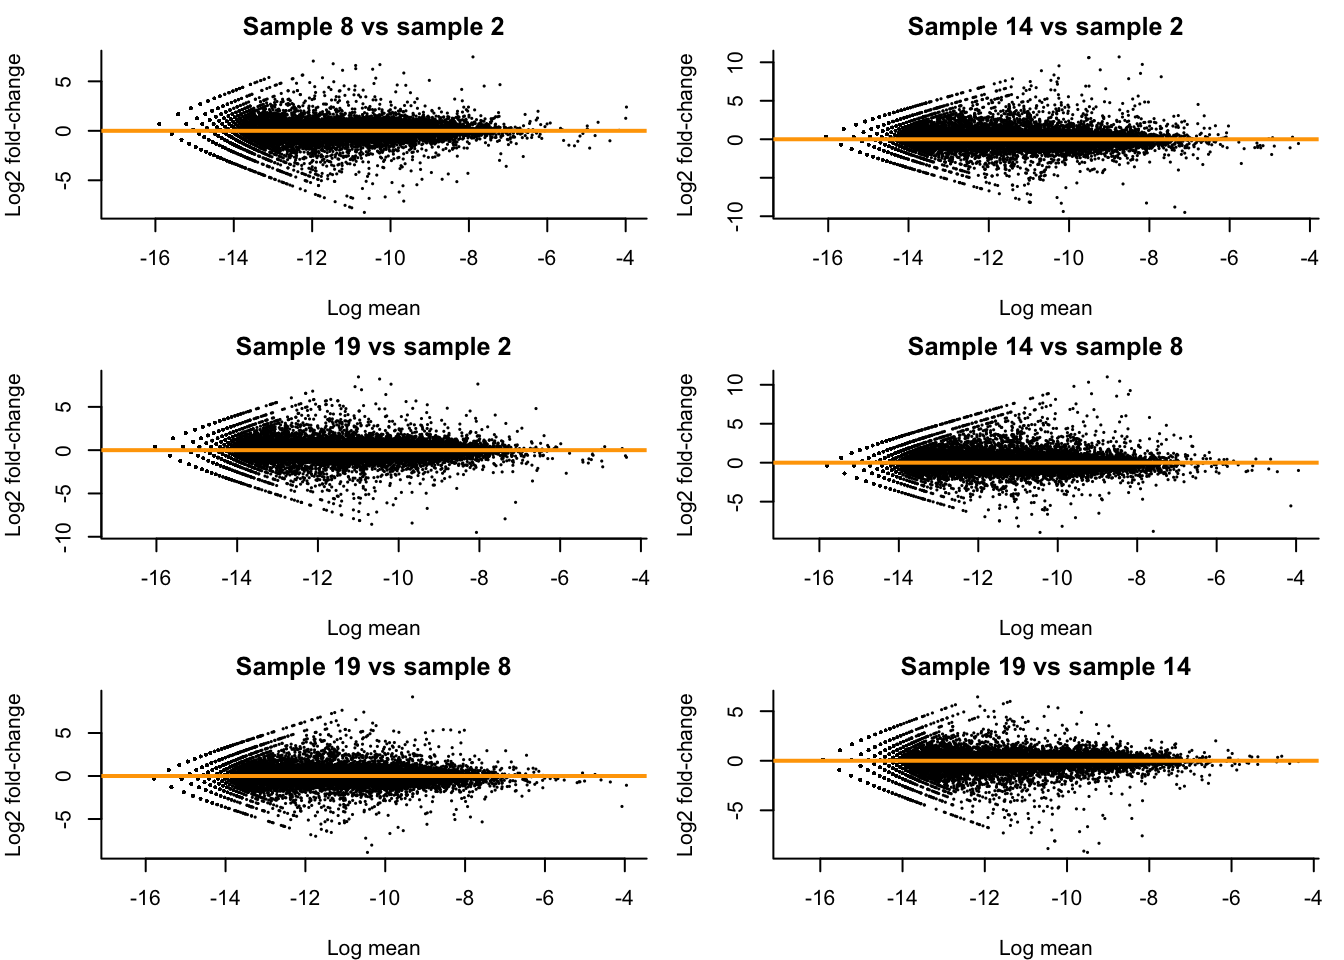
\includegraphics{sequencing_rnaseqIntro_files/figure-beamer/unnamed-chunk-12-1.pdf}

\end{block}

\end{block}

\begin{block}{Median-of-ratios method (default of \texttt{DESeq2})}

The median-of-ratios method is used in \texttt{DESeq2} as described in
\href{https://genomebiology.biomedcentral.com/articles/10.1186/s13059-014-0550-8}{Love
\emph{et al.} (2014)}. It assumes that the expected value
\(\mu_{gi} = E(Y_{gi})\) is proportional to the true expression of the
gene, \(q_{gi}\), scaled by a normalization factor \(s_{i}\) for each
sample, \[ \mu_{gi} = s_{i}q_{gi}. \]

The normalization factor \(s_{i}\) is then estimated using the
median-of-ratios method compared to a synthetic reference sample \(r\)
defined based on geometric means of counts across samples \[
s_i = \text{median}_{\{{g:Y^{*}_{gr} \ne 0}\}} \frac{Y_{gi}}{Y^{*}_{gr}},
\] with \[ Y^{*}_{gr} = \left( \prod_{i=1}^n Y_{gi} \right)^{1/n}. \]
From this, we calculate the normalized count as
\(\tilde{Y}_{gi} = Y_{gi} / s_{i}\).

Median-of-ratios normalization is implemented in the \texttt{DESeq2}
package:

\begin{Shaded}
\begin{Highlighting}[]
\NormalTok{dds <-}\StringTok{ }\NormalTok{DESeq2}\OperatorTok{::}\KeywordTok{DESeqDataSetFromMatrix}\NormalTok{(}\DataTypeTok{countData =} \KeywordTok{assays}\NormalTok{(se)}\OperatorTok{$}\NormalTok{counts,}
                                      \DataTypeTok{colData =} \KeywordTok{colData}\NormalTok{(se),}
                                      \DataTypeTok{design =} \OperatorTok{~}\StringTok{ }\DecValTok{1}\NormalTok{) }\CommentTok{#just add intercept to showcase normalization}
\end{Highlighting}
\end{Shaded}

\begin{verbatim}
## converting counts to integer mode
\end{verbatim}

\begin{Shaded}
\begin{Highlighting}[]
\NormalTok{dds <-}\StringTok{ }\NormalTok{DESeq2}\OperatorTok{::}\KeywordTok{estimateSizeFactors}\NormalTok{(dds)}
\KeywordTok{sizeFactors}\NormalTok{(dds)}
\end{Highlighting}
\end{Shaded}

\begin{verbatim}
##  [1] 0.9187624 1.0644717 0.5232069 0.9826698 0.5676212 0.7807662 0.8284089
##  [8] 0.6600848 2.3955069 0.7906917 2.2784591 0.7860386 0.7807842 0.8445577
## [15] 1.3345483 1.7011973 2.5001652 0.7889061 0.8138720 0.7632306 1.4518320
## [22] 0.6553677 1.6696064
\end{verbatim}

You may also want to check out the
\href{https://www.youtube.com/watch?v=UFB993xufUU}{StatQuest video on
DESeq2 normalization}.

\end{block}

\begin{block}{Full quantile (FQ) normalization}

In full-quantile normalization, originally introduced in the context of
microarrays by
\href{https://academic.oup.com/bioinformatics/article/19/2/185/372664}{Bolstad
\emph{et al.} (2003)}, the samples are forced to each have a
distribution identical to the distribution of the median/average of the
quantiles across samples. In practice, we implement full-quantile
normalization using the following procedure

\begin{enumerate}
\tightlist
\item
  Given a data matrix \(\mathbf{Y}_{G \times n}\) for \(G\) genes (rows)
  and \(n\) samples (columns),
\item
  sort each column to get \(\mathbf{Y}^S\),
\item
  replace all elements of each row by the median (or average) for that
  row,
\item
  obtain the normalized counts \(\tilde{\mathbf{Y}}\) by re-arranging
  (i.e., unsorting) each column.
\end{enumerate}

\end{block}

\begin{block}{Conditional quantile normalization (\texttt{cqn})}

The \texttt{cqn} method, introduced by
\href{https://academic.oup.com/biostatistics/article/13/2/204/1746212}{Hansen
\emph{et al.} (2012)} and implemented in the \texttt{cqn} \texttt{R}
package, starts by assuming a Poisson model for the gene expression
counts \(Y_{gi}\). Median regression is used to model, for each sample,
the log-transformed accessibility count as a smooth function of
GC-content as well as gene length, focusing on genes with high average
count (above \(50\) by default). Next, subset quantile normalization
(\href{https://www.liebertpub.com/doi/10.1089/cmb.2010.0049}{Wu \emph{et
al.} (2010)}) is performed on the residuals of that model (i.e., on the
counts adjusted for GC-content) for between-sample normalization. The
method could intuitively be thought of as full-quantile normalization
after removing a smoothed sample-specific GC-content effect. Normalized
counts are calculated as recommended in the \texttt{cqn} vignette, i.e.,
\[
\tilde{Y}_{gi} = \left(\frac{(Y_{gi}+1) 10^6}{\sum_g Y_{gi}}\right)  2^{O_{gi}},
\] with \(O_{gi}\) the normalization offset estimated by \texttt{cqn},
which is on the \(\log_2\) scale. Note that \texttt{cqn} normalization
works with a gene- and sample-specific offset, unlike TMM and
median-of-ratios normalization which only work with a sample-specific
offset.

\end{block}

\end{frame}

\begin{frame}[fragile]{Challenge III: Parameter estimation (under
limited information setting)}
\protect\hypertarget{challenge-iii-parameter-estimation-under-limited-information-setting}{}

There are two challenges to be overcome here. First, we need to get the
structure of our mean model right, this is, which covariates to include,
and how to include them, such that we are capable of capturing important
sources of variation in our experiment, in order to derive a correct
interpretation of the data in terms of our research question.

Second, we need to be able to estimate the parameters of our model in an
efficient way, while having limited information (i.e., we only have a
small number of replicates).

\begin{block}{Defining the model for the mean}

Let's first check how the authors of the original study parameterized
the mean model.

\begin{figure}
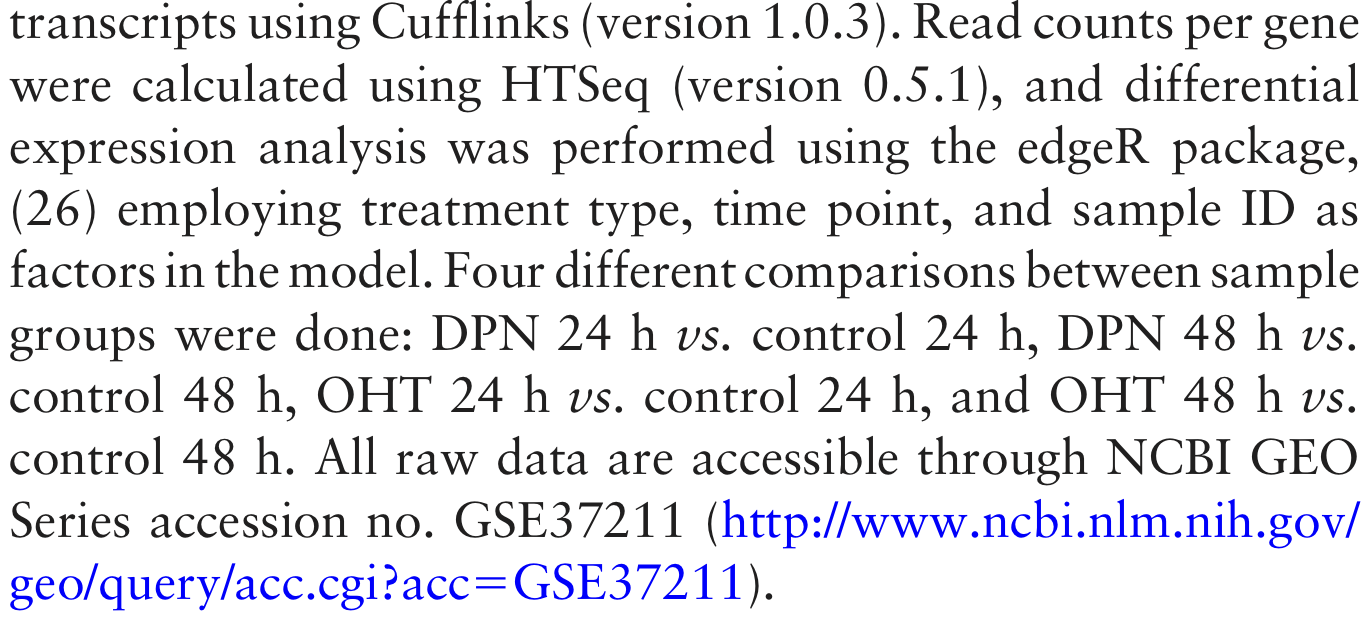
\includegraphics[width=18.97in]{./images_sequencing/deAnalysis_para} \caption{Figure: Another paragraph from the Methods section.}\label{fig:unnamed-chunk-14}
\end{figure}

The authors write that they are ``employing treatment type, time point
and sample ID as factors in the model''. Concerning experimental
variables, this suggests they have added covariates defining the
treatment and time point for each sample. The sample ID in the text
refers to the original tissue sample and therefore corresponds to the
donor patient. While there is also a variable called \texttt{sample} in
the \texttt{colData}, this is not what the authors refer to. Note the
ambiguity here and since the authors didn't share their code, this is
hard to check! But, more on reproducibility later.

\textbf{Question}. What are the authors assuming using this structure
for the mean model? Do you think that there are extensions or
simplifications of the mean model that would be relevant?

 Answer.

The authors are acknowledging the relatedness of samples derived from
the same donor patient by adding it as a fixed effect to the model,
which is great. This blocking strategy has been extensively discussed in
the proteomics part of this course. However, by only adding a main
effect for treatment and time, they are assuming that the effect of time
is identical for all treatments, i.e., the average gene expression
in-/decrease at 48h versus 24h is identical for the DPN, OHT or the
control samples, which seems like a quite stringent assumption. We can
make the model more flexible (but also more complex) by allowing for a
\texttt{treatment\ *\ time} interaction.

\end{block}

\begin{block}{Parameter estimation and empirical Bayes}

Even in limited sample sizes, the parameters \(\beta\) of the mean model
may be estimated reasonably efficiently. However, estimating parameters
for the varaince (this is, the dispersion parameter \(\phi\) from the
negative binomial or the variance parameter \(\sigma\) from the
Gaussian) are typically quite a bit harder.

In genomics, we often take advantage of the parallel structure of the
thousands of regression models (one for each gene) to \textbf{borrow
information across genes} in a procedure called \textbf{empirical
Bayes}, as also seen in the proteomics part of this course. In empirical
Bayes, we basically take a semi-Bayesian approach to parameter
estimation, where we use the data but also a prior distribution to
derive our parameter estimate. However, what makes it empirical is that
we are using the data to estimate this prior distribution, unlike in a
fully Bayesian analysis where the prior distribution must be specified
independently of the data. The basic assumption for this to make sense
is that genes with similar means might have similar dispersion
parameters (or variances), owing to the mean-variance trend.

Once initial estimates (\(\hat{\Phi}_g^{ML}\) in the figure) have been
derived, we use a parametric model to estimate its distribution
(typically as a function of the mean), which we're calling the prior
distribution. Then, each initial estimate is shrunken towards that
empirically estimated prior distribution. The amount of shrinkage being
performed is data-driven, and depends on the data, taking into account
the precision of our initial estimate (i.e., shape of the likelihood)
and the width of the prior.

These strategies result in impressive performance gains in terms of
differential expression analysis and are implemented in all popular
differential expression analysis software packages (though in slightly
differing ways) like \texttt{limma}, \texttt{edgeR} and \texttt{DESeq2}.

\begin{figure}
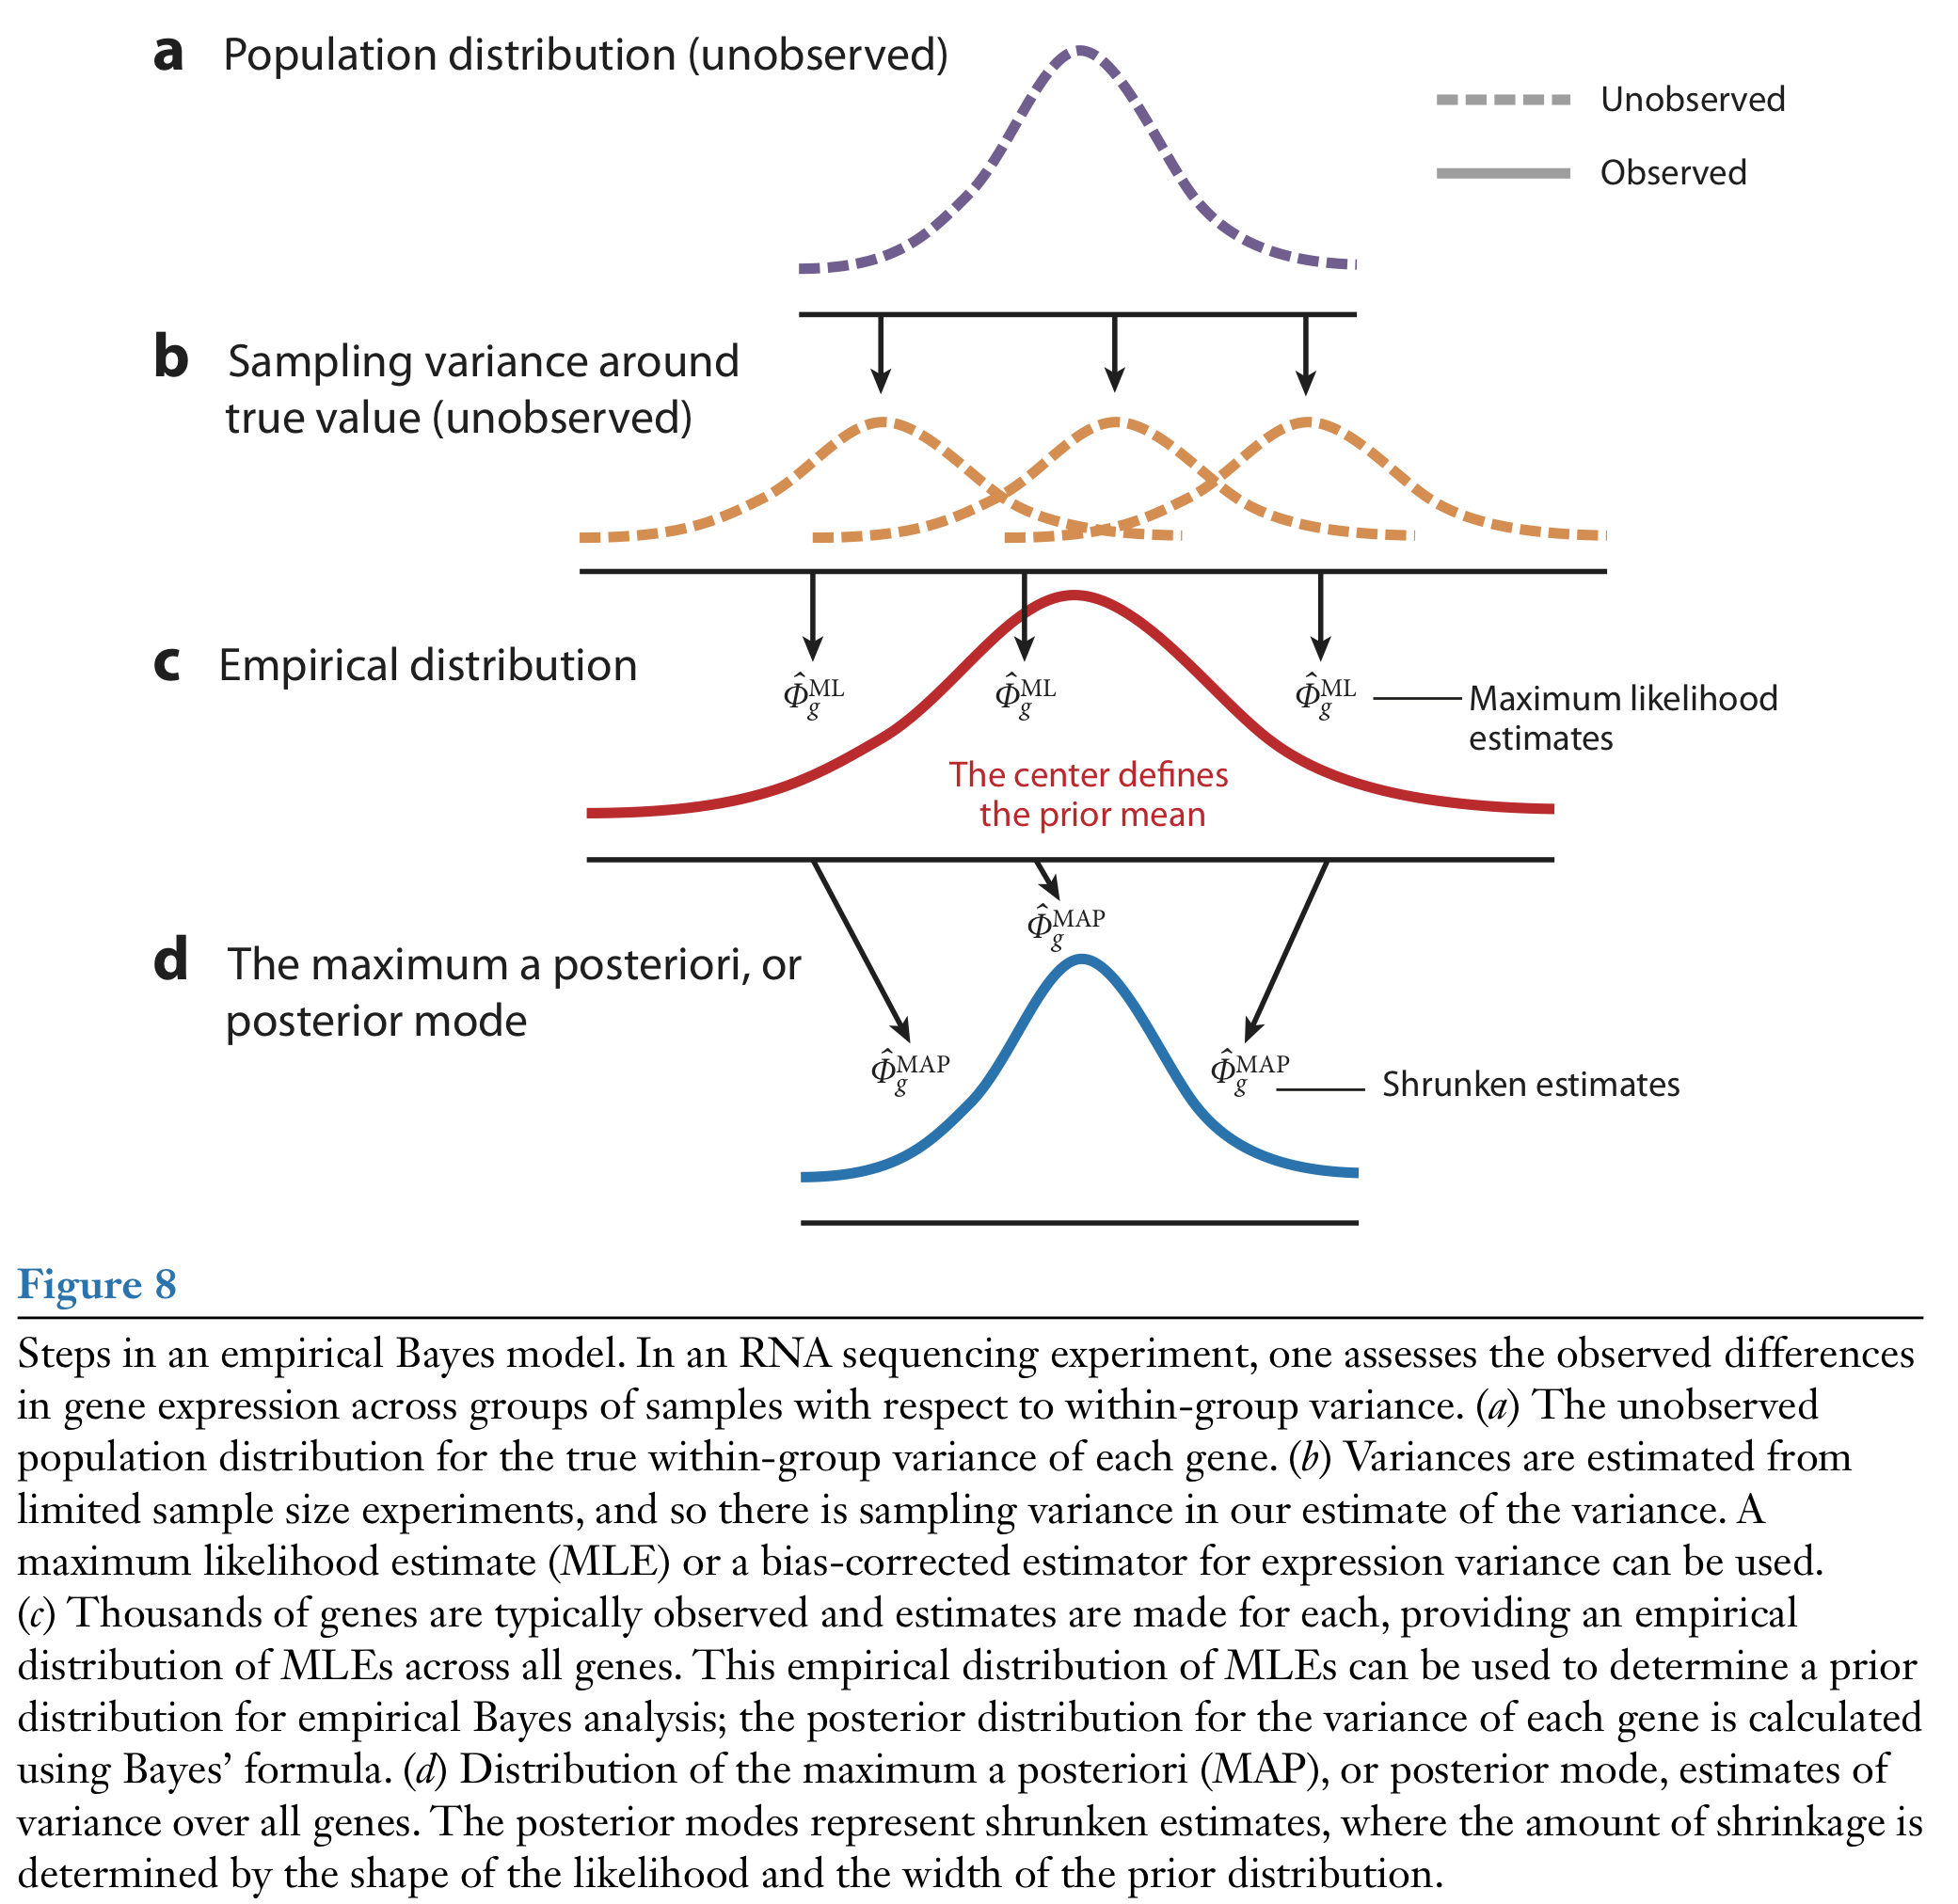
\includegraphics[width=28.9in]{./images_sequencing/empiricalBayes} \caption{Figure 8 from Van den Berge *et al.* (2019).}\label{fig:unnamed-chunk-15}
\end{figure}

\end{block}

\begin{block}{In practice}

Let's fit the model using \texttt{edgeR}.

\begin{Shaded}
\begin{Highlighting}[]
\NormalTok{design <-}\StringTok{ }\KeywordTok{model.matrix}\NormalTok{(}\OperatorTok{~}\StringTok{ }\NormalTok{treatment}\OperatorTok{*}\NormalTok{time }\OperatorTok{+}\StringTok{ }\NormalTok{patient, }\DataTypeTok{data=}\KeywordTok{colData}\NormalTok{(se))}

\CommentTok{# independent filtering}
\NormalTok{keep <-}\StringTok{ }\KeywordTok{filterByExpr}\NormalTok{(se, }\DataTypeTok{design =}\NormalTok{ design)}
\NormalTok{se <-}\StringTok{ }\NormalTok{se[keep,]}

\NormalTok{dge <-}\StringTok{ }\KeywordTok{calcNormFactors}\NormalTok{(se)}
\NormalTok{dge <-}\StringTok{ }\KeywordTok{estimateDisp}\NormalTok{(dge, design) }\CommentTok{# estimate dispersion estimates}
\KeywordTok{plotBCV}\NormalTok{(dge)}
\end{Highlighting}
\end{Shaded}

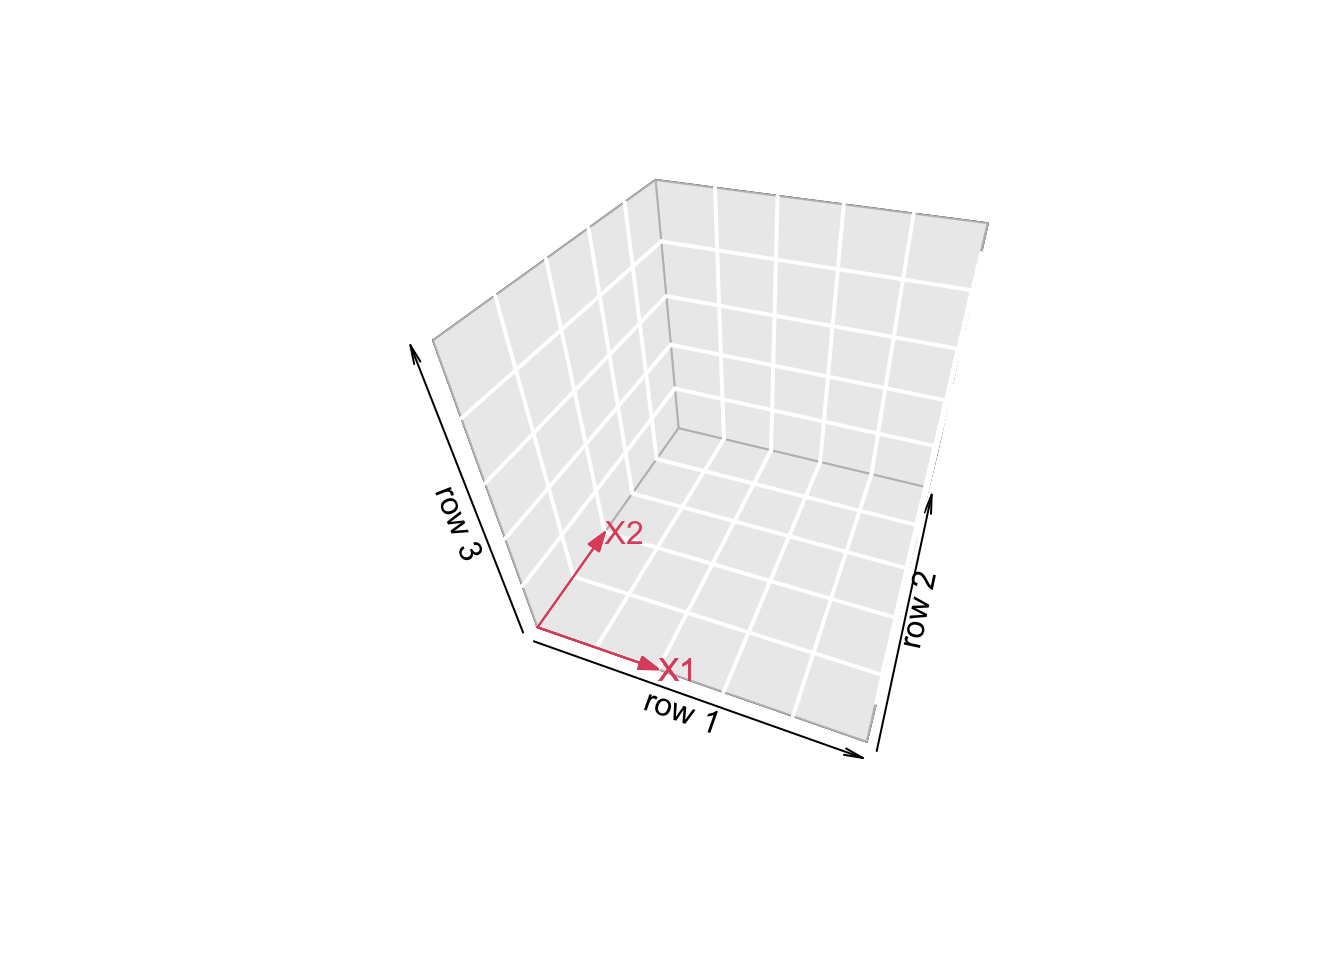
\includegraphics{sequencing_rnaseqIntro_files/figure-beamer/unnamed-chunk-16-1.pdf}

\begin{Shaded}
\begin{Highlighting}[]
\NormalTok{fit <-}\StringTok{ }\KeywordTok{glmFit}\NormalTok{(dge, design)}
\KeywordTok{head}\NormalTok{(fit}\OperatorTok{$}\NormalTok{coefficients)}
\end{Highlighting}
\end{Shaded}

\begin{verbatim}
##                 (Intercept) treatmentDPN treatmentOHT     time48h   patient2
## ENSG00000000003   -9.331882   0.11123447   0.08546850  0.13117317 -0.5174796
## ENSG00000000419  -10.373781  -0.05315770  -0.03584722 -0.09477144  0.1387269
## ENSG00000000457  -10.934527  -0.12862571  -0.13423965 -0.07529975  0.4584629
## ENSG00000000460  -10.097504   0.08765191   0.13668806 -0.89531654  0.5419252
## ENSG00000000938  -14.696298   0.02065948  -0.08388580  0.34012665  1.4483041
## ENSG00000000971  -13.686862   0.29231910   0.26552992  0.48915000 -0.1460052
##                    patient3   patient4 treatmentDPN:time48h
## ENSG00000000003 -0.83223188 -0.6265133           -0.1218237
## ENSG00000000419  0.10284160  0.1003775            0.0491583
## ENSG00000000457 -0.05968439  0.2070947            0.0646111
## ENSG00000000460 -0.33688177 -0.1340312            0.1601642
## ENSG00000000938  0.53981205  0.8188658           -0.1240420
## ENSG00000000971  0.93631262 -0.2692062           -0.6029327
##                 treatmentOHT:time48h
## ENSG00000000003           -0.1183197
## ENSG00000000419            0.1167476
## ENSG00000000457            0.1322449
## ENSG00000000460            0.1829253
## ENSG00000000938           -0.2098209
## ENSG00000000971           -0.7136537
\end{verbatim}

\end{block}

\end{frame}

\begin{frame}[fragile]{Challenge IV: Statistical inference across many
genes}
\protect\hypertarget{challenge-iv-statistical-inference-across-many-genes}{}

\begin{block}{Contrasts on the treatment effects}

We will first derive all contrasts that are also investigated in the
original manuscript, using our extended model where we are allowing for
an interaction effect between treatment and time.

The mean model is
\[ \log(\mu_{gi}) = \beta_{g0} + \beta_{g1} x_{DPN} + \beta_{g2} x_{OHT} + \beta_{g3} x_{48h} + \beta_{g4} x_{pat2} + \beta_{g5} x_{pat3} + \beta_{g6} x_{pat4} + \beta_{g7} x_{DPN:48h} + \beta_{g8} x_{OHT:48h}. \]

The intercept corresponds to the log average gene expression in the
control group at 24h for patient 1.

\textbf{DPN 24h vs control 24h.} The respective means are
\[\log \mu_{g,DPN,24h} = \beta_{g0} + \beta_{g1},\]
\[\log \mu_{g,con,24h} = \beta_{g0}.\] And their difference is
\[ \delta_g = \beta_{g1}. \]

\textbf{DPN 48h vs control 48h.} The respective means are
\[\log \mu_{g,DPN,48h} = \beta_{g0} + \beta_{g1} + \beta_{g3} + \beta_{g7},\]
\[\log \mu_{g,con,48h} = \beta_{g0} + \beta_{g3}.\] And their difference
is \[ \delta_g = \beta_{g1} + \beta_{g7}. \]

\textbf{OHT 24h vs control 24h.} The respective means are
\[\log \mu_{g,OHT,24h} = \beta_{g0} + \beta_{g2} ,\]
\[\log \mu_{g,con,24h} = \beta_{g0}.\] And their difference is
\[ \delta_g = \beta_{g2}. \]

\textbf{OHT 48h vs control 48h.} The respective means are
\[\log \mu_{g,OHT,48h} = \beta_{g0} + \beta_{g2} + \beta_{g3} + \beta_{g8},\]
\[\log \mu_{g,con,48h} = \beta_{g0} + \beta_{g3}.\] And their difference
is \[ \delta_g = \beta_{g2} + \beta_{g8}. \]

However, we can also assess the interaction effects: is the time effect
different between DPN and OHT treatment versus the control? And how
about the DPN vs OHT treatments?

\textbf{DPN vs control interaction.} The time effect for each condition
is
\[ \delta_{DPN} = \log \mu_{g,DPN,48h} - \log \mu_{g,DPN,24h} = \beta_{g3} + \beta_{g7},\]
\[ \delta_{con} = \log \mu_{g,con,48h} - \log \mu_{g,con,24h} = \beta_{g3}. \]
So the interaction effect is \[\delta_{DPN-con} = \beta_{g7}.\]

\textbf{OHT vs control interaction.} The time effect for each condition
is
\[ \delta_{OHT} = \log \mu_{g,OHT,48h} - \log \mu_{g,OHT,24h} = \beta_{g3} + \beta_{g8},\]
\[ \delta_{con} = \log \mu_{g,con,48h} - \log \mu_{g,con,24h} = \beta_{g3}. \]
So the interaction effect is \[\delta_{DPN-con} = \beta_{g8}.\]

\textbf{OHT vs DPN interaction.} The time effect for each condition is
\[ \delta_{OHT} = \log \mu_{g,OHT,48h} - \log \mu_{g,OHT,24h} = \beta_{g3} + \beta_{g8},\]
\[ \delta_{DPN} = \log \mu_{g,DPN,48h} - \log \mu_{g,DPN,24h} = \beta_{g3} + \beta_{g7},\]
So the interaction effect is
\[\delta_{OHT-DPN} = \beta_{g8} - \beta_{g7}.\]

Let's implement all of these in a contrast matrix.

\begin{Shaded}
\begin{Highlighting}[]
\NormalTok{L <-}\StringTok{ }\KeywordTok{matrix}\NormalTok{(}\DecValTok{0}\NormalTok{, }\DataTypeTok{nrow =} \KeywordTok{ncol}\NormalTok{(fit}\OperatorTok{$}\NormalTok{coefficients), }\DataTypeTok{ncol =} \DecValTok{7}\NormalTok{)}
\KeywordTok{rownames}\NormalTok{(L) <-}\StringTok{ }\KeywordTok{colnames}\NormalTok{(fit}\OperatorTok{$}\NormalTok{coefficients)}
\KeywordTok{colnames}\NormalTok{(L) <-}\StringTok{ }\KeywordTok{c}\NormalTok{(}\StringTok{"DPNvsCON24"}\NormalTok{, }\StringTok{"DPNvsCON48"}\NormalTok{,}
                 \StringTok{"OHTvsCON24"}\NormalTok{, }\StringTok{"OHTvsCON48"}\NormalTok{,}
                 \StringTok{"DPNvsCONInt"}\NormalTok{, }\StringTok{"OHTvsCONInt"}\NormalTok{,}
                 \StringTok{"OHTvsDPNInt"}\NormalTok{)}
\CommentTok{# DPN vs control at 24h}
\NormalTok{L[}\DecValTok{2}\NormalTok{,}\StringTok{"DPNvsCON24"}\NormalTok{] <-}\StringTok{ }\DecValTok{1}
\CommentTok{# DPN vs control at 48h}
\NormalTok{L[}\KeywordTok{c}\NormalTok{(}\DecValTok{2}\NormalTok{,}\DecValTok{8}\NormalTok{),}\StringTok{"DPNvsCON48"}\NormalTok{] <-}\StringTok{ }\DecValTok{1}
\CommentTok{# OHT vs control at 24h}
\NormalTok{L[}\DecValTok{3}\NormalTok{,}\StringTok{"OHTvsCON24"}\NormalTok{] <-}\StringTok{ }\DecValTok{1}
\CommentTok{# OHT vs control at 48h}
\NormalTok{L[}\KeywordTok{c}\NormalTok{(}\DecValTok{3}\NormalTok{,}\DecValTok{9}\NormalTok{),}\StringTok{"OHTvsCON48"}\NormalTok{] <-}\StringTok{ }\DecValTok{1}
\CommentTok{# DPN control interaction}
\NormalTok{L[}\DecValTok{8}\NormalTok{,}\StringTok{"DPNvsCONInt"}\NormalTok{] <-}\StringTok{ }\DecValTok{1}
\CommentTok{# OHT control interaction}
\NormalTok{L[}\DecValTok{9}\NormalTok{,}\StringTok{"OHTvsCONInt"}\NormalTok{] <-}\StringTok{ }\DecValTok{1}
\CommentTok{# OHT DPN interaction}
\NormalTok{L[}\KeywordTok{c}\NormalTok{(}\DecValTok{9}\NormalTok{,}\DecValTok{8}\NormalTok{),}\StringTok{"OHTvsDPNInt"}\NormalTok{] <-}\StringTok{ }\KeywordTok{c}\NormalTok{(}\DecValTok{1}\NormalTok{, }\DecValTok{-1}\NormalTok{)}

\NormalTok{L}
\end{Highlighting}
\end{Shaded}

\begin{verbatim}
##                      DPNvsCON24 DPNvsCON48 OHTvsCON24 OHTvsCON48 DPNvsCONInt
## (Intercept)                   0          0          0          0           0
## treatmentDPN                  1          1          0          0           0
## treatmentOHT                  0          0          1          1           0
## time48h                       0          0          0          0           0
## patient2                      0          0          0          0           0
## patient3                      0          0          0          0           0
## patient4                      0          0          0          0           0
## treatmentDPN:time48h          0          1          0          0           1
## treatmentOHT:time48h          0          0          0          1           0
##                      OHTvsCONInt OHTvsDPNInt
## (Intercept)                    0           0
## treatmentDPN                   0           0
## treatmentOHT                   0           0
## time48h                        0           0
## patient2                       0           0
## patient3                       0           0
## patient4                       0           0
## treatmentDPN:time48h           0          -1
## treatmentOHT:time48h           1           1
\end{verbatim}

And, finally, we can assess each hypothesis using the \texttt{glmLRT}
function implemented in \texttt{edgeR}. We can assess each hypothesis
separately by looping over the contrasts.

\begin{Shaded}
\begin{Highlighting}[]
\NormalTok{lrtList <-}\StringTok{ }\KeywordTok{list}\NormalTok{() }\CommentTok{#list of results}
\ControlFlowTok{for}\NormalTok{(cc }\ControlFlowTok{in} \DecValTok{1}\OperatorTok{:}\KeywordTok{ncol}\NormalTok{(L)) lrtList[[cc]] <-}\StringTok{ }\KeywordTok{glmLRT}\NormalTok{(fit, }\DataTypeTok{contrast =}\NormalTok{ L[,cc])}

\CommentTok{# p-value histograms}
\NormalTok{pvalList <-}\StringTok{ }\KeywordTok{lapply}\NormalTok{(lrtList, }\ControlFlowTok{function}\NormalTok{(x) x}\OperatorTok{$}\NormalTok{table}\OperatorTok{$}\NormalTok{PValue)}
\NormalTok{pvalMat <-}\StringTok{ }\KeywordTok{do.call}\NormalTok{(cbind,  pvalList)}
\KeywordTok{colnames}\NormalTok{(pvalMat) <-}\StringTok{ }\KeywordTok{colnames}\NormalTok{(L)}
\KeywordTok{par}\NormalTok{(}\DataTypeTok{mfrow=}\KeywordTok{c}\NormalTok{(}\DecValTok{3}\NormalTok{,}\DecValTok{3}\NormalTok{))}
\KeywordTok{sapply}\NormalTok{(}\DecValTok{1}\OperatorTok{:}\KeywordTok{ncol}\NormalTok{(pvalMat), }\ControlFlowTok{function}\NormalTok{(ii) }\KeywordTok{hist}\NormalTok{(pvalMat[,ii], }
                                          \DataTypeTok{main =} \KeywordTok{colnames}\NormalTok{(pvalMat)[ii],}
                                          \DataTypeTok{xlab =} \StringTok{"p-value"}\NormalTok{))}
\end{Highlighting}
\end{Shaded}

\begin{verbatim}
##          [,1]            [,2]            [,3]            [,4]           
## breaks   Numeric,21      Numeric,21      Numeric,21      Numeric,21     
## counts   Integer,20      Integer,20      Integer,20      Integer,20     
## density  Numeric,20      Numeric,20      Numeric,20      Numeric,20     
## mids     Numeric,20      Numeric,20      Numeric,20      Numeric,20     
## xname    "pvalMat[, ii]" "pvalMat[, ii]" "pvalMat[, ii]" "pvalMat[, ii]"
## equidist TRUE            TRUE            TRUE            TRUE           
##          [,5]            [,6]            [,7]           
## breaks   Numeric,21      Numeric,21      Numeric,21     
## counts   Integer,20      Integer,20      Integer,20     
## density  Numeric,20      Numeric,20      Numeric,20     
## mids     Numeric,20      Numeric,20      Numeric,20     
## xname    "pvalMat[, ii]" "pvalMat[, ii]" "pvalMat[, ii]"
## equidist TRUE            TRUE            TRUE
\end{verbatim}

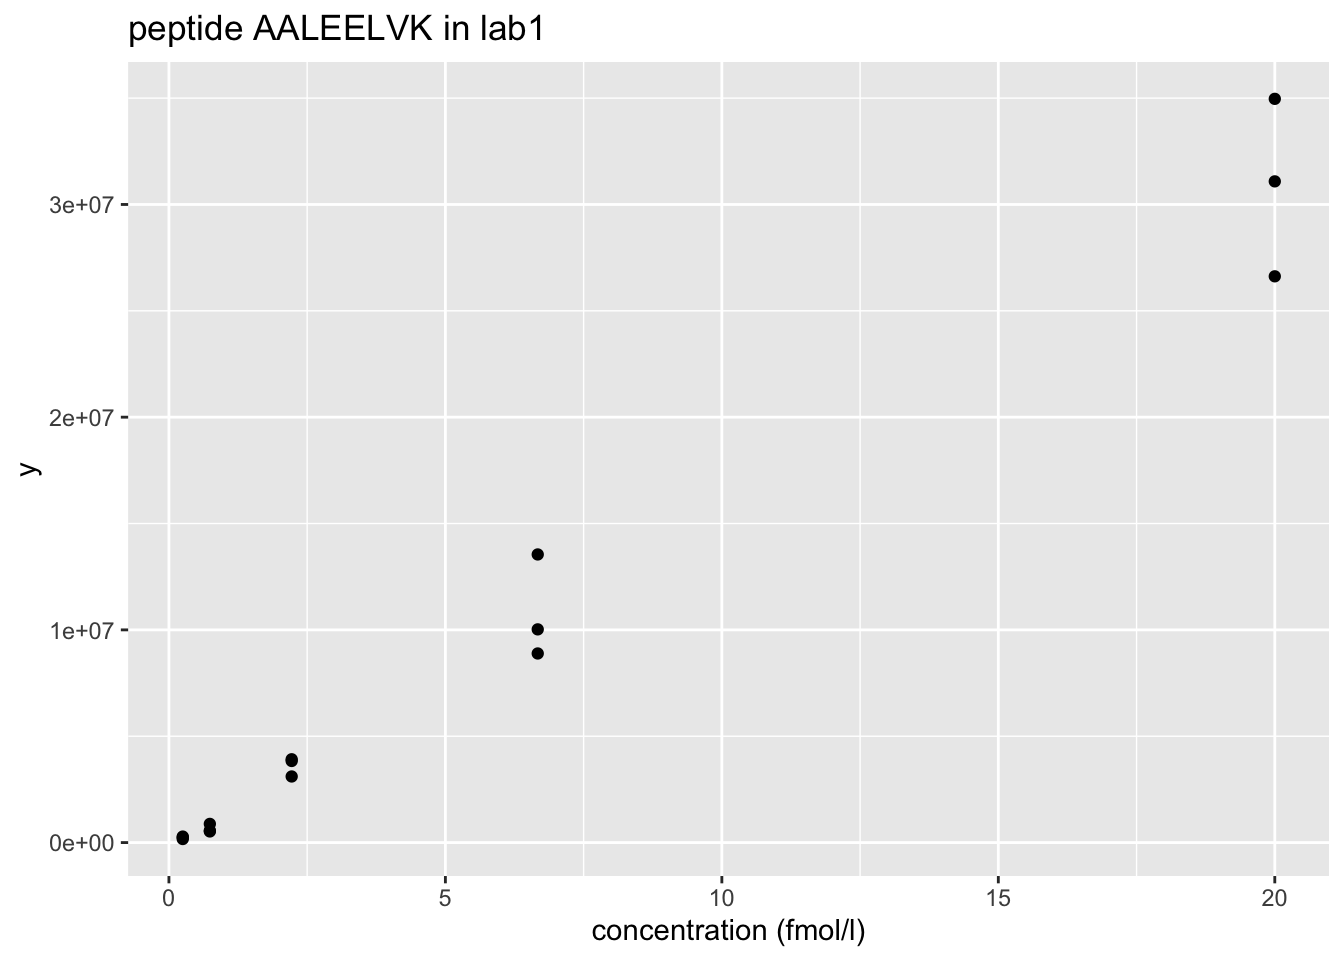
\includegraphics{sequencing_rnaseqIntro_files/figure-beamer/unnamed-chunk-18-1.pdf}

\begin{block}{Multiple testing}

\begin{Shaded}
\begin{Highlighting}[]
\CommentTok{# number of DE genes}
\NormalTok{padjMat <-}\StringTok{ }\KeywordTok{apply}\NormalTok{(pvalMat, }\DecValTok{2}\NormalTok{, p.adjust, }\DataTypeTok{method=}\StringTok{"fdr"}\NormalTok{)}
\KeywordTok{colSums}\NormalTok{(padjMat }\OperatorTok{<=}\StringTok{ }\FloatTok{0.05}\NormalTok{ )}
\end{Highlighting}
\end{Shaded}

\begin{verbatim}
##  DPNvsCON24  DPNvsCON48  OHTvsCON24  OHTvsCON48 DPNvsCONInt OHTvsCONInt 
##           2          64           0          23           0           0 
## OHTvsDPNInt 
##           0
\end{verbatim}

We are finding low numbers of DE genes between treatments at a 5\% FDR
level. This was already reflected in the the MDS plots.

\end{block}

\begin{block}{Visualization}

Let's visualize some results for the DPN vs control at 48h contrast.

\begin{Shaded}
\begin{Highlighting}[]
\KeywordTok{library}\NormalTok{(scales) }\CommentTok{# for scales::alpha()}
\NormalTok{deGenes <-}\StringTok{ }\KeywordTok{p.adjust}\NormalTok{(lrtList[[}\DecValTok{2}\NormalTok{]]}\OperatorTok{$}\NormalTok{table}\OperatorTok{$}\NormalTok{PValue, }\StringTok{"fdr"}\NormalTok{) }\OperatorTok{<=}\StringTok{ }\FloatTok{0.05}

\CommentTok{## volcano plot}
\KeywordTok{plot}\NormalTok{(}\DataTypeTok{x =}\NormalTok{ lrtList[[}\DecValTok{2}\NormalTok{]]}\OperatorTok{$}\NormalTok{table}\OperatorTok{$}\NormalTok{logFC,}
     \DataTypeTok{y =} \OperatorTok{-}\KeywordTok{log10}\NormalTok{(lrtList[[}\DecValTok{2}\NormalTok{]]}\OperatorTok{$}\NormalTok{table}\OperatorTok{$}\NormalTok{PValue),}
     \DataTypeTok{xlab =} \StringTok{"log Fold-change"}\NormalTok{,}
     \DataTypeTok{ylab =} \StringTok{"-log10 P-value"}\NormalTok{,}
     \DataTypeTok{pch =} \DecValTok{16}\NormalTok{, }\DataTypeTok{col =} \KeywordTok{alpha}\NormalTok{(deGenes}\OperatorTok{+}\DecValTok{1}\NormalTok{, }\FloatTok{.4}\NormalTok{), }
     \DataTypeTok{cex=}\DecValTok{2}\OperatorTok{/}\DecValTok{3}\NormalTok{, }\DataTypeTok{bty=}\StringTok{'l'}\NormalTok{)}
\KeywordTok{legend}\NormalTok{(}\StringTok{"topright"}\NormalTok{, }\KeywordTok{c}\NormalTok{(}\StringTok{"DE"}\NormalTok{, }\StringTok{"not DE"}\NormalTok{),}
       \DataTypeTok{col =} \DecValTok{2}\OperatorTok{:}\DecValTok{1}\NormalTok{, }\DataTypeTok{pch=}\DecValTok{16}\NormalTok{, }\DataTypeTok{bty=}\StringTok{'n'}\NormalTok{)}
\end{Highlighting}
\end{Shaded}

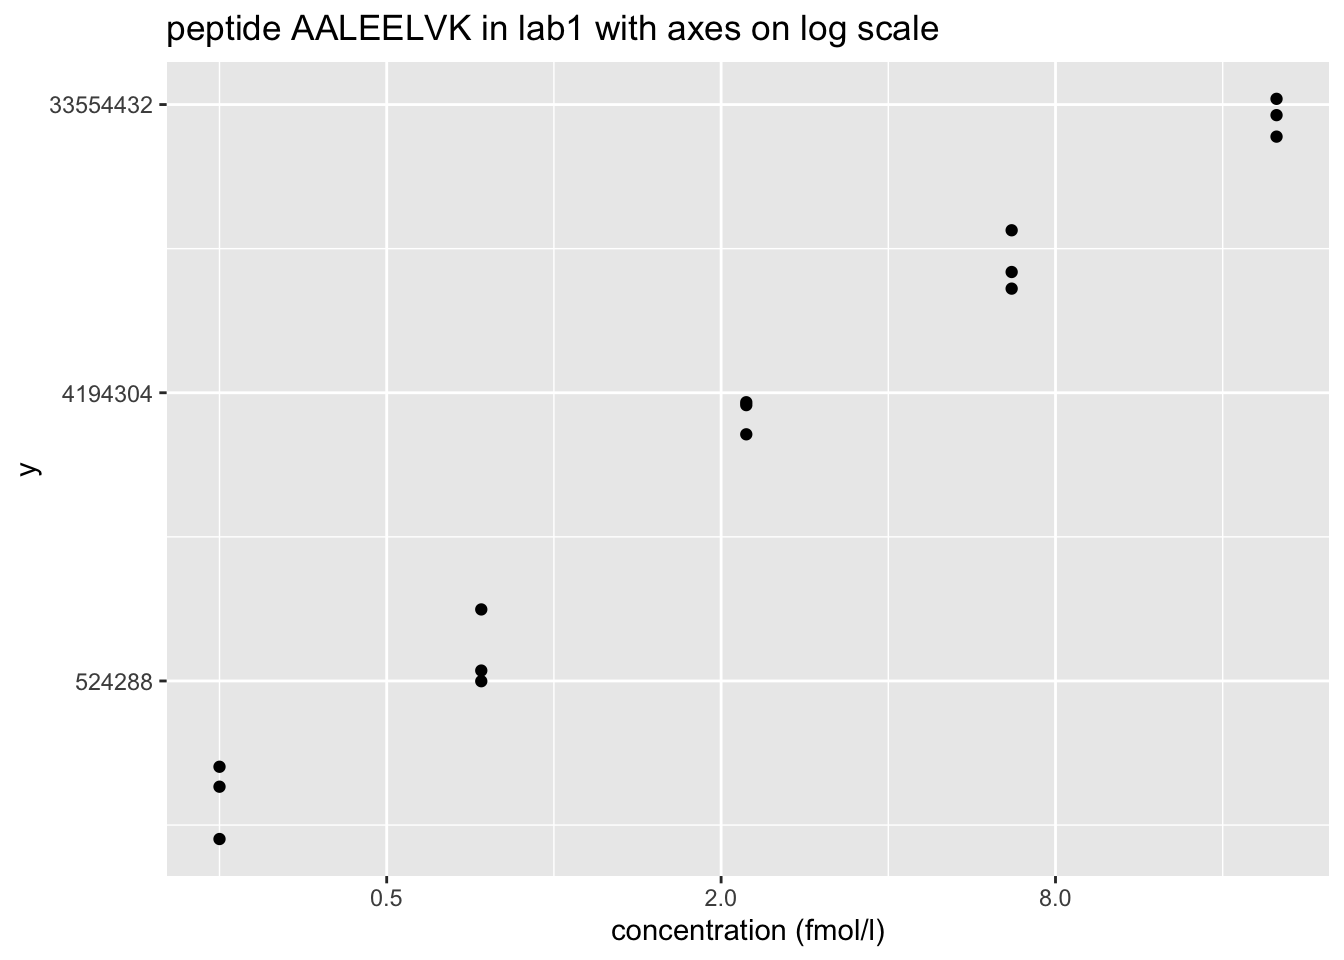
\includegraphics{sequencing_rnaseqIntro_files/figure-beamer/unnamed-chunk-20-1.pdf}

\begin{Shaded}
\begin{Highlighting}[]
\CommentTok{## MD-plot}
\KeywordTok{plot}\NormalTok{(}\DataTypeTok{x =}\NormalTok{ lrtList[[}\DecValTok{2}\NormalTok{]]}\OperatorTok{$}\NormalTok{table}\OperatorTok{$}\NormalTok{logCPM,}
     \DataTypeTok{y =}\NormalTok{ lrtList[[}\DecValTok{2}\NormalTok{]]}\OperatorTok{$}\NormalTok{table}\OperatorTok{$}\NormalTok{logFC,}
     \DataTypeTok{xlab =} \StringTok{"Average log CPM"}\NormalTok{,}
     \DataTypeTok{ylab =} \StringTok{"Log fold-change"}\NormalTok{,}
     \DataTypeTok{pch =} \DecValTok{16}\NormalTok{, }\DataTypeTok{col =} \KeywordTok{alpha}\NormalTok{(deGenes}\OperatorTok{+}\DecValTok{1}\NormalTok{, }\FloatTok{.4}\NormalTok{), }
     \DataTypeTok{cex=}\DecValTok{2}\OperatorTok{/}\DecValTok{3}\NormalTok{, }\DataTypeTok{bty=}\StringTok{'l'}\NormalTok{)}
\KeywordTok{legend}\NormalTok{(}\StringTok{"topright"}\NormalTok{, }\KeywordTok{c}\NormalTok{(}\StringTok{"DE"}\NormalTok{, }\StringTok{"not DE"}\NormalTok{),}
       \DataTypeTok{col =} \DecValTok{2}\OperatorTok{:}\DecValTok{1}\NormalTok{, }\DataTypeTok{pch=}\DecValTok{16}\NormalTok{, }\DataTypeTok{bty=}\StringTok{'n'}\NormalTok{)}
\KeywordTok{abline}\NormalTok{(}\DataTypeTok{h=}\DecValTok{0}\NormalTok{, }\DataTypeTok{col=}\StringTok{"orange"}\NormalTok{, }\DataTypeTok{lwd=}\DecValTok{2}\NormalTok{, }\DataTypeTok{lty=}\DecValTok{2}\NormalTok{)}
\end{Highlighting}
\end{Shaded}

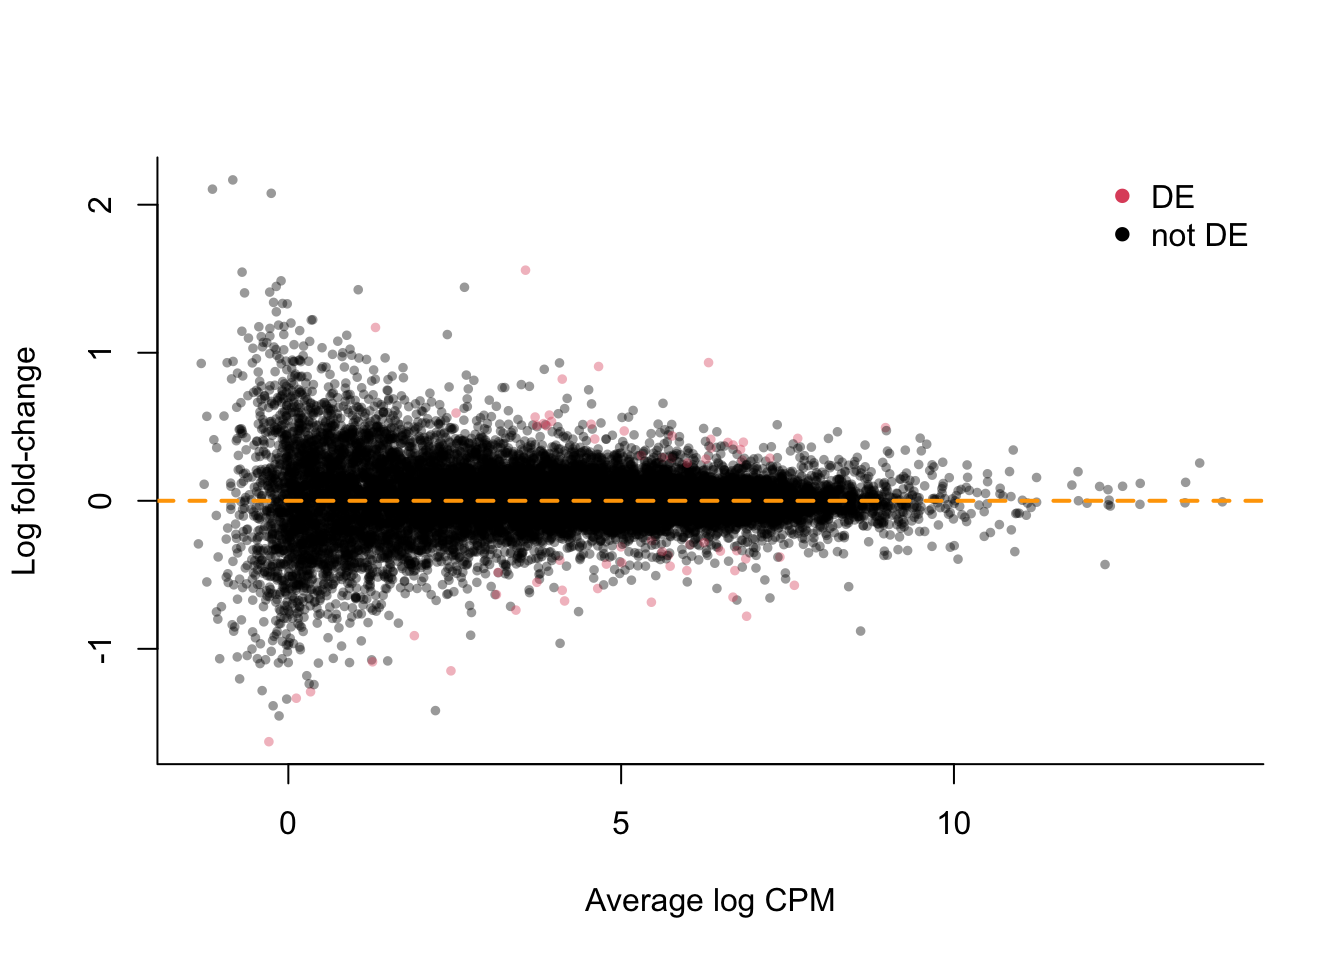
\includegraphics{sequencing_rnaseqIntro_files/figure-beamer/unnamed-chunk-20-2.pdf}

\end{block}

\end{block}

\end{frame}

\begin{frame}[fragile]

\begin{Shaded}
\begin{Highlighting}[]
\CommentTok{# extract all DE genes}
\NormalTok{deGenes <-}\StringTok{ }\KeywordTok{rownames}\NormalTok{(lrtList[[}\DecValTok{2}\NormalTok{]]}\OperatorTok{$}\NormalTok{table)[}\KeywordTok{p.adjust}\NormalTok{(lrtList[[}\DecValTok{2}\NormalTok{]]}\OperatorTok{$}\NormalTok{table}\OperatorTok{$}\NormalTok{PValue, }\StringTok{"fdr"}\NormalTok{) }\OperatorTok{<=}\StringTok{ }\FloatTok{0.05}\NormalTok{]}
\NormalTok{deGenes}
\end{Highlighting}
\end{Shaded}

\begin{verbatim}
##  [1] "ENSG00000035928" "ENSG00000044574" "ENSG00000070882" "ENSG00000075790"
##  [5] "ENSG00000091137" "ENSG00000092621" "ENSG00000099864" "ENSG00000099875"
##  [9] "ENSG00000100219" "ENSG00000100867" "ENSG00000101255" "ENSG00000101974"
## [13] "ENSG00000102547" "ENSG00000103064" "ENSG00000103257" "ENSG00000103449"
## [17] "ENSG00000107796" "ENSG00000111181" "ENSG00000111790" "ENSG00000119242"
## [21] "ENSG00000120129" "ENSG00000120217" "ENSG00000133935" "ENSG00000135069"
## [25] "ENSG00000135473" "ENSG00000135541" "ENSG00000138685" "ENSG00000143127"
## [29] "ENSG00000145050" "ENSG00000145244" "ENSG00000149428" "ENSG00000149485"
## [33] "ENSG00000152952" "ENSG00000155111" "ENSG00000155330" "ENSG00000155660"
## [37] "ENSG00000164597" "ENSG00000166813" "ENSG00000167608" "ENSG00000167703"
## [41] "ENSG00000168014" "ENSG00000169174" "ENSG00000169239" "ENSG00000169762"
## [45] "ENSG00000170122" "ENSG00000170837" "ENSG00000171798" "ENSG00000172935"
## [49] "ENSG00000173210" "ENSG00000175198" "ENSG00000181790" "ENSG00000182704"
## [53] "ENSG00000182836" "ENSG00000183401" "ENSG00000185818" "ENSG00000187908"
## [57] "ENSG00000188783" "ENSG00000197976" "ENSG00000219481" "ENSG00000226887"
## [61] "ENSG00000233705" "ENSG00000234431" "ENSG00000236044" "ENSG00000243927"
\end{verbatim}

\begin{Shaded}
\begin{Highlighting}[]
\CommentTok{# order according to absolute fold-change}
\NormalTok{orderedDEGenes <-}\StringTok{ }\NormalTok{deGenes[}\KeywordTok{order}\NormalTok{(}\KeywordTok{abs}\NormalTok{(lrtList[[}\DecValTok{2}\NormalTok{]]}\OperatorTok{$}\NormalTok{table[deGenes, }\StringTok{"logFC"}\NormalTok{]), }\DataTypeTok{decreasing =} \OtherTok{TRUE}\NormalTok{)]}

\KeywordTok{par}\NormalTok{(}\DataTypeTok{mfrow=}\KeywordTok{c}\NormalTok{(}\DecValTok{3}\NormalTok{,}\DecValTok{3}\NormalTok{))}
\ControlFlowTok{for}\NormalTok{(kk }\ControlFlowTok{in} \DecValTok{1}\OperatorTok{:}\KeywordTok{length}\NormalTok{(orderedDEGenes))\{}
  \KeywordTok{boxplot}\NormalTok{(}\KeywordTok{log1p}\NormalTok{(}\KeywordTok{assays}\NormalTok{(se)}\OperatorTok{$}\NormalTok{counts[orderedDEGenes[kk],]) }\OperatorTok{~}\StringTok{ }\KeywordTok{interaction}\NormalTok{(treatment, time))}
  \KeywordTok{boxplot}\NormalTok{(fit}\OperatorTok{$}\NormalTok{fitted.values[orderedDEGenes[kk],] }\OperatorTok{~}\StringTok{ }\KeywordTok{interaction}\NormalTok{(treatment, time))}
\NormalTok{\}}
\end{Highlighting}
\end{Shaded}

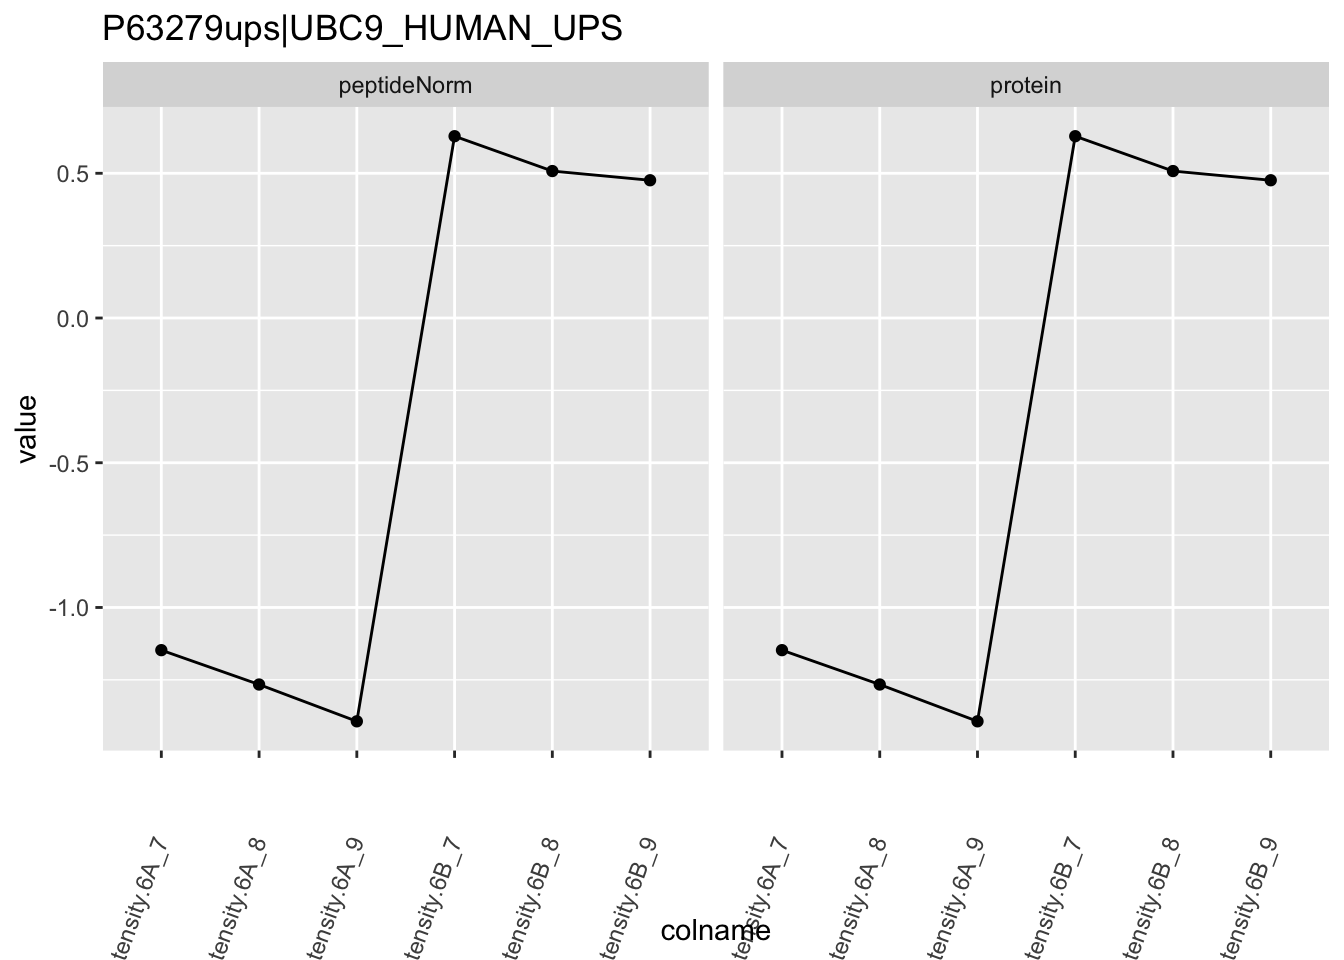
\includegraphics{sequencing_rnaseqIntro_files/figure-beamer/unnamed-chunk-21-1.pdf}
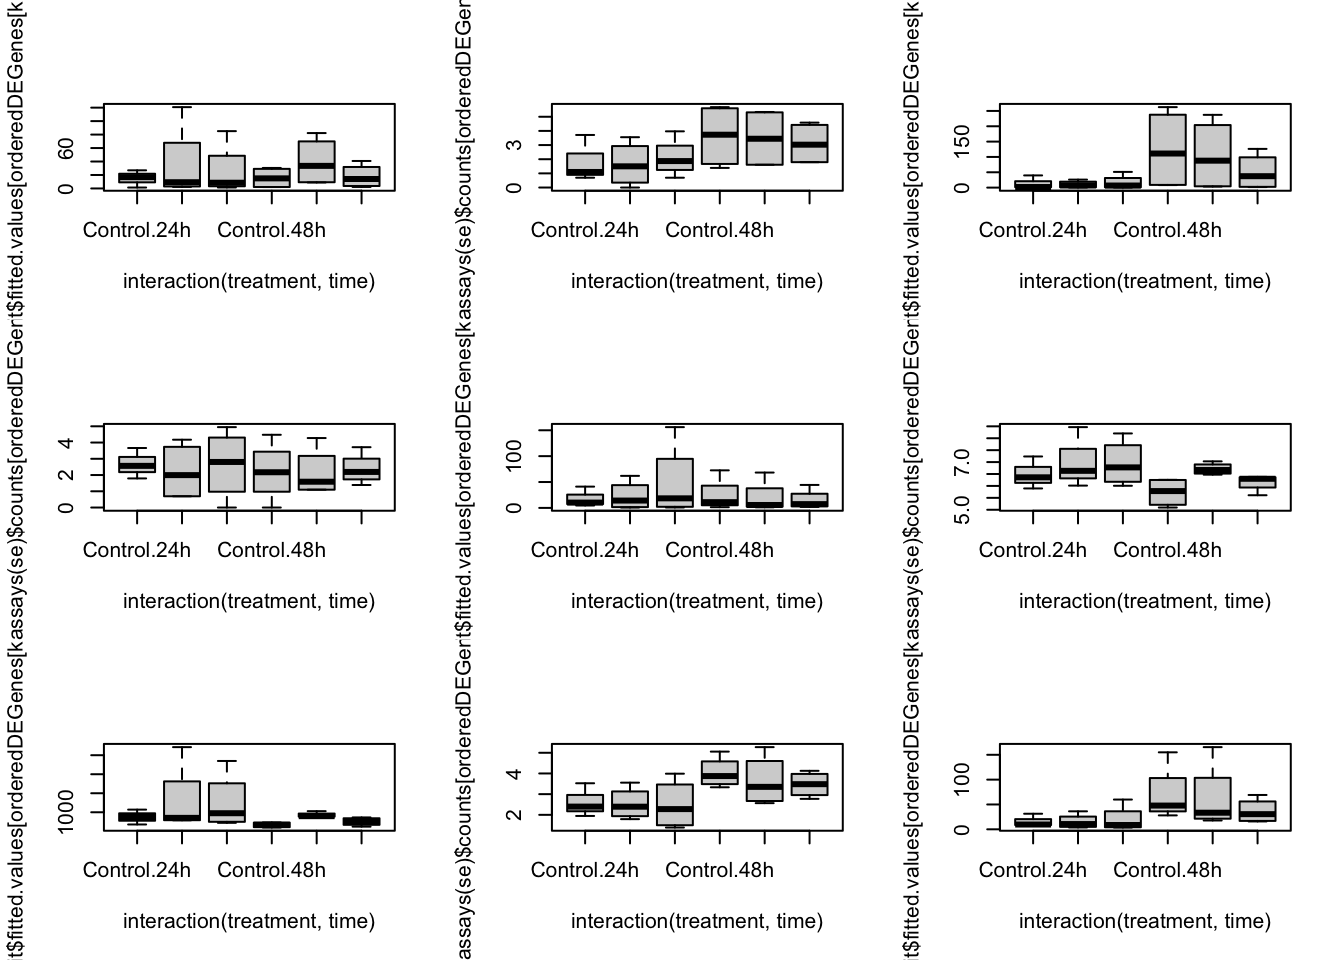
\includegraphics{sequencing_rnaseqIntro_files/figure-beamer/unnamed-chunk-21-2.pdf}
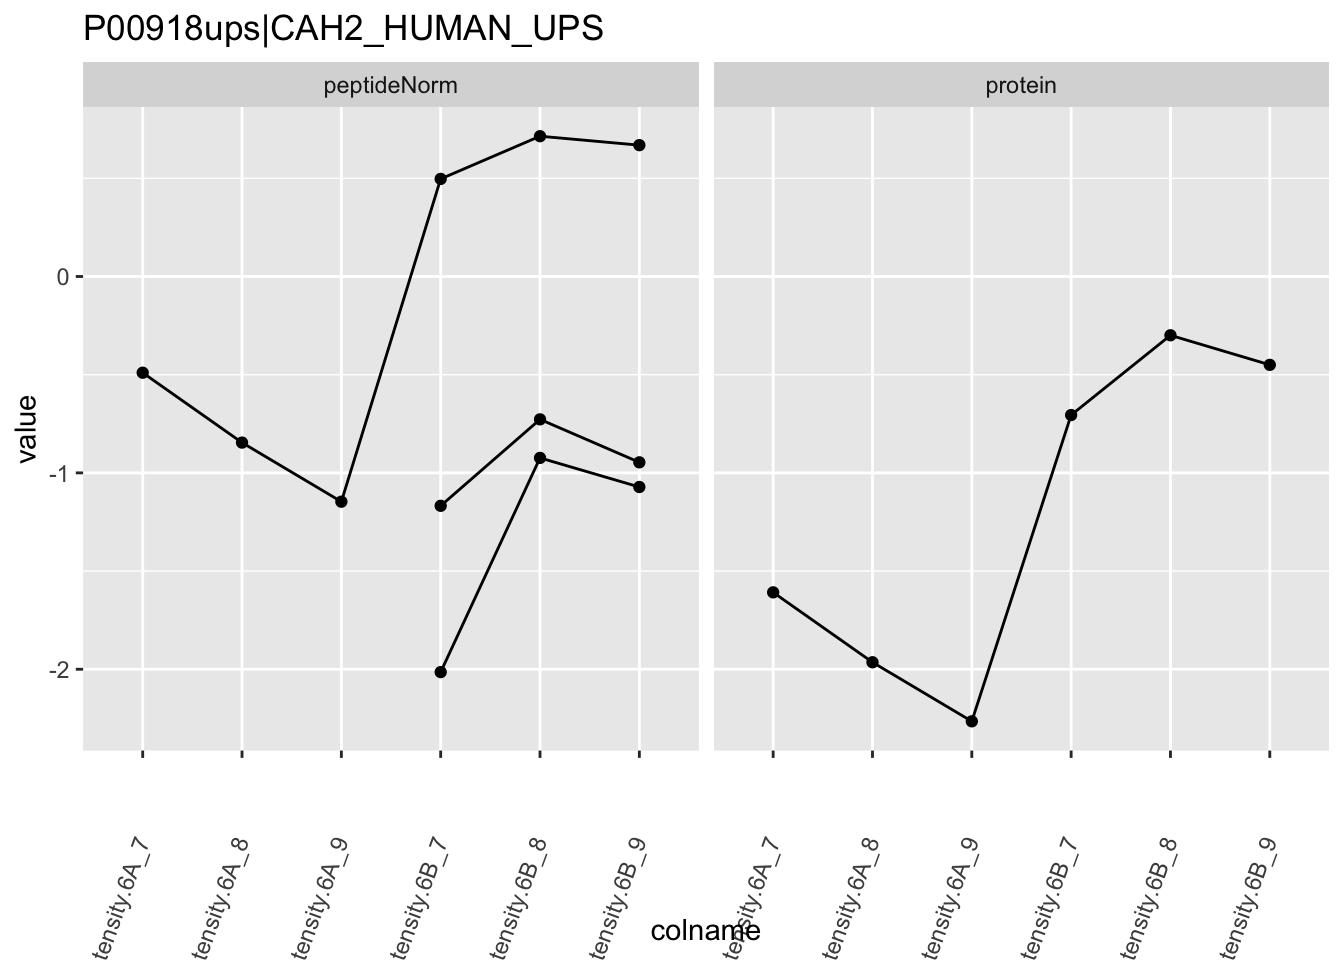
\includegraphics{sequencing_rnaseqIntro_files/figure-beamer/unnamed-chunk-21-3.pdf}
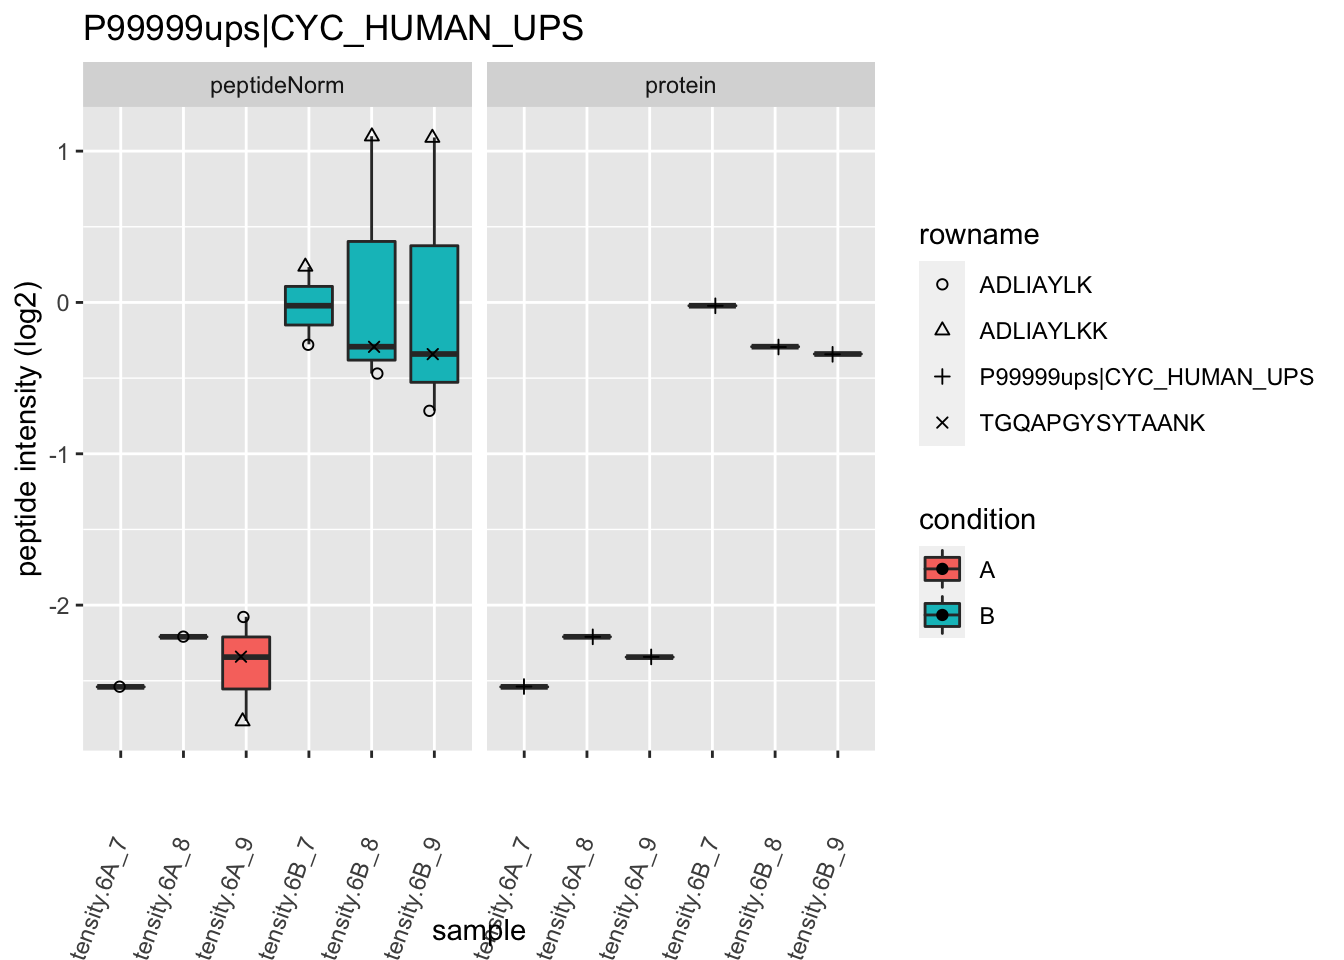
\includegraphics{sequencing_rnaseqIntro_files/figure-beamer/unnamed-chunk-21-4.pdf}
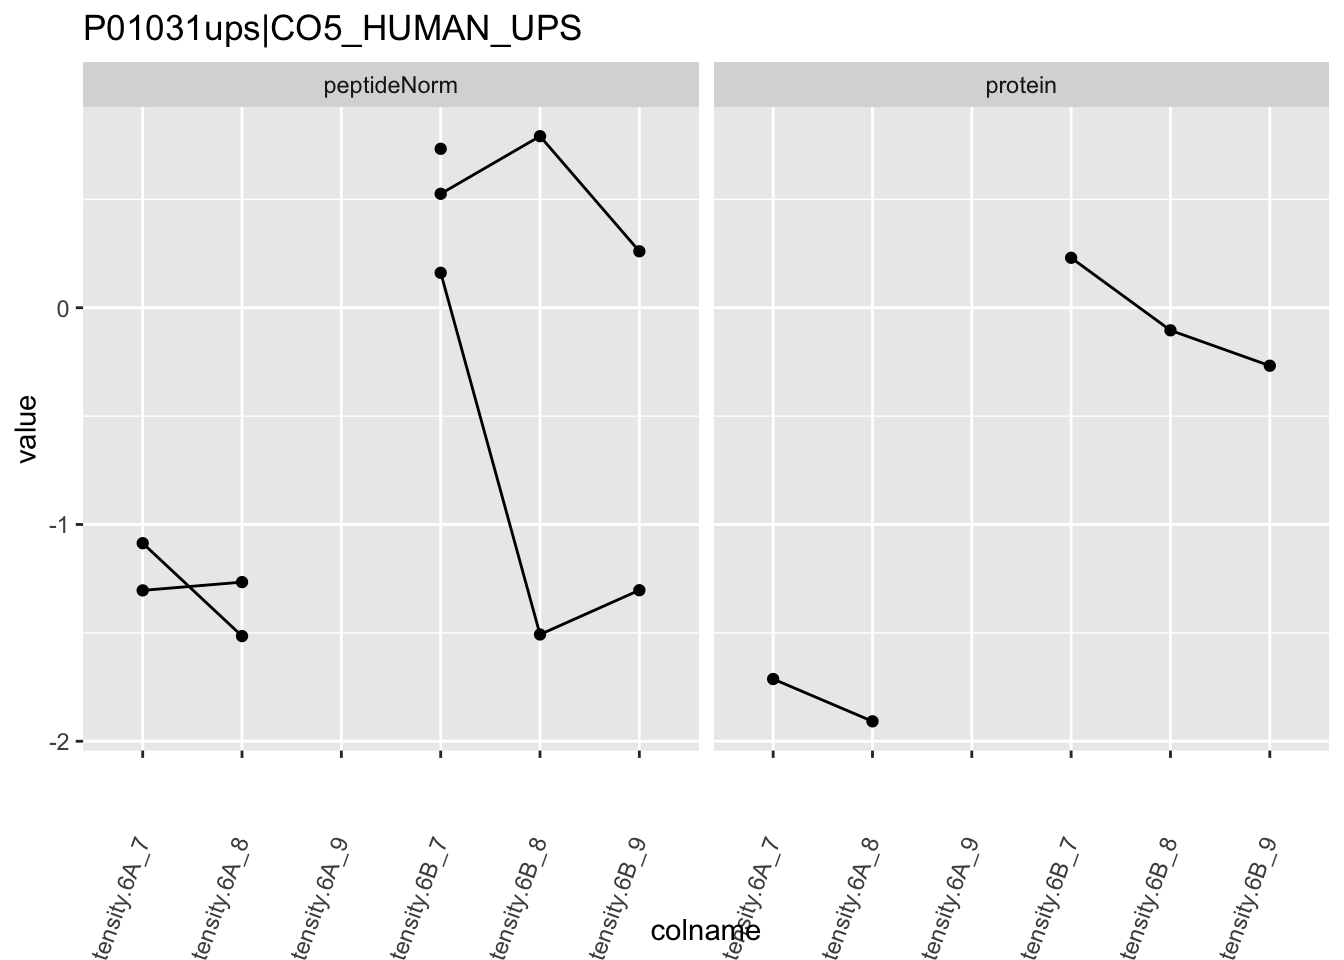
\includegraphics{sequencing_rnaseqIntro_files/figure-beamer/unnamed-chunk-21-5.pdf}
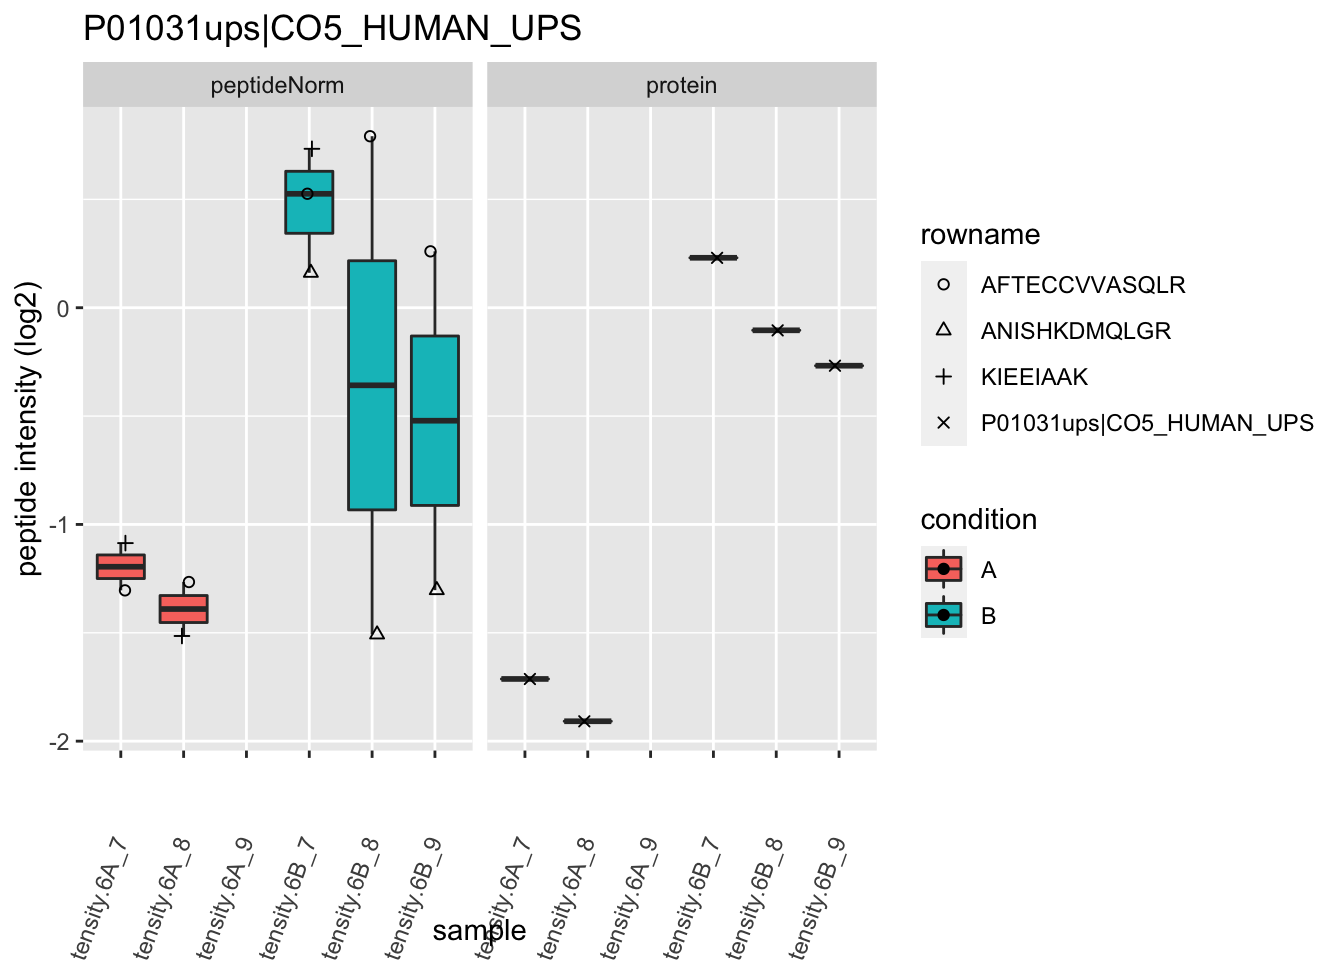
\includegraphics{sequencing_rnaseqIntro_files/figure-beamer/unnamed-chunk-21-6.pdf}
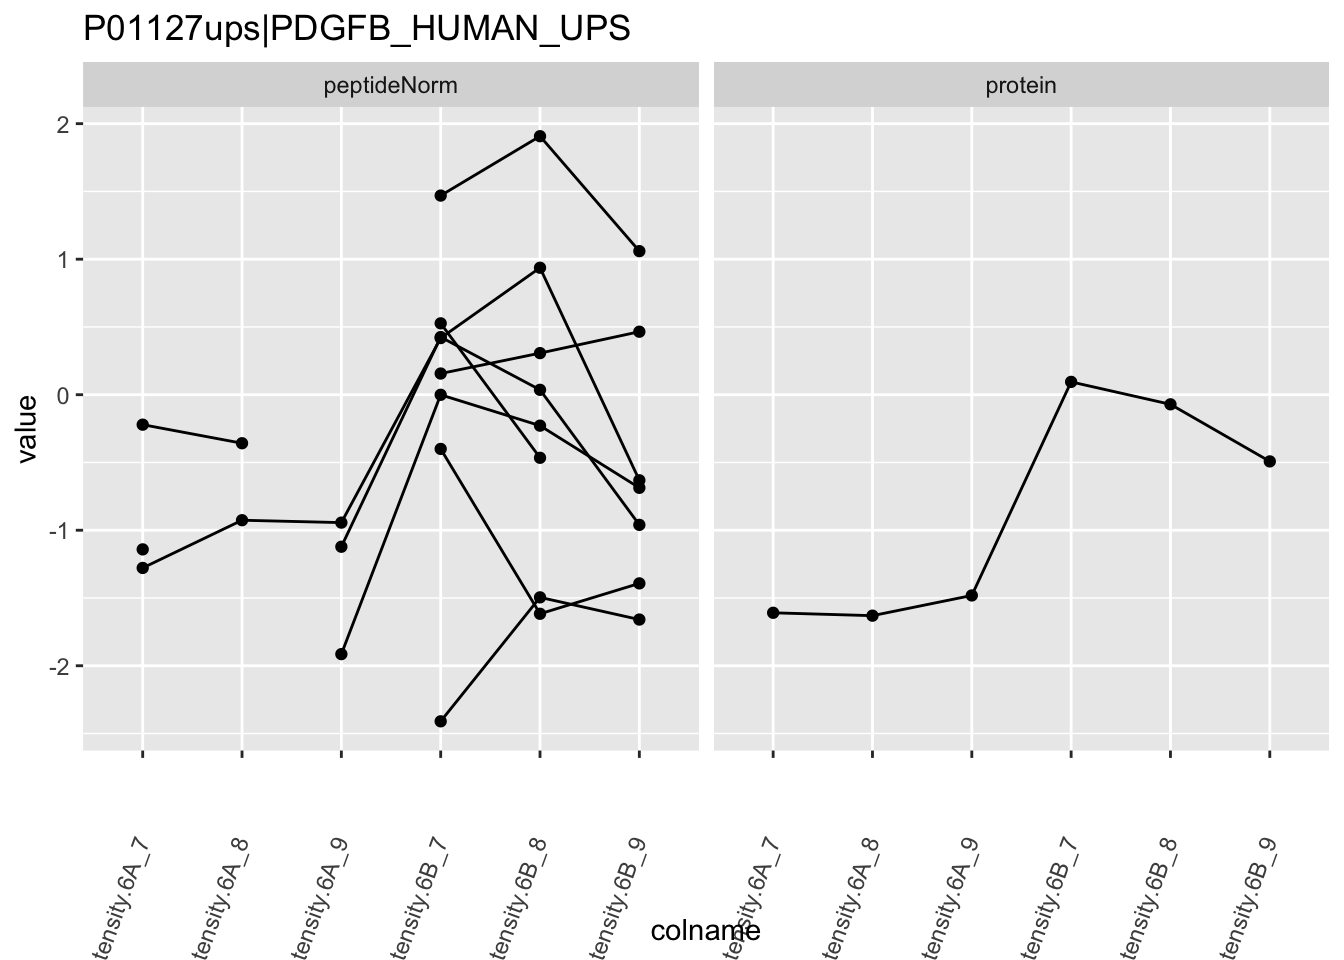
\includegraphics{sequencing_rnaseqIntro_files/figure-beamer/unnamed-chunk-21-7.pdf}
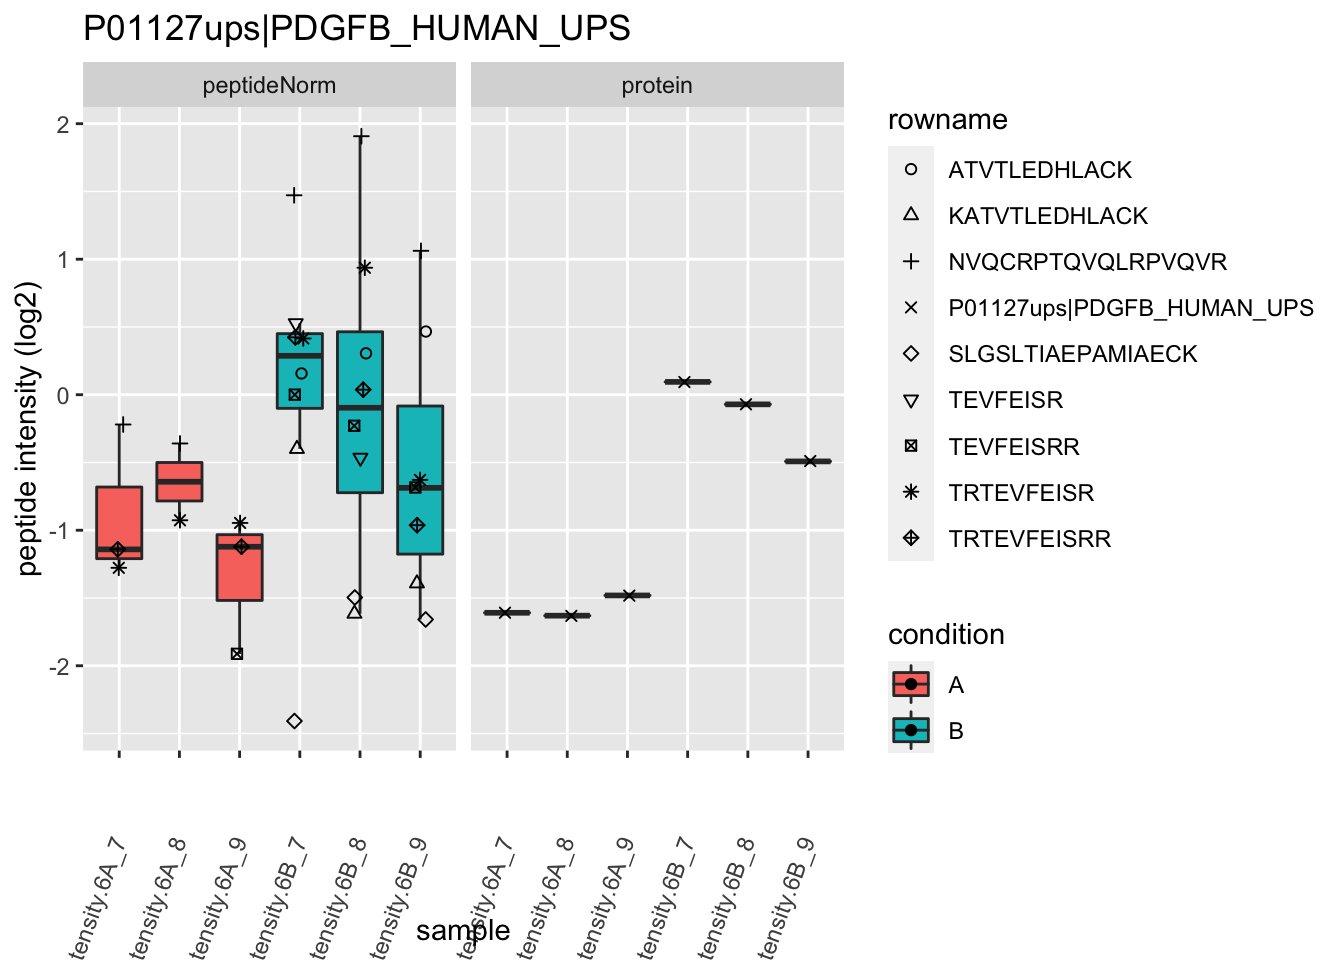
\includegraphics{sequencing_rnaseqIntro_files/figure-beamer/unnamed-chunk-21-8.pdf}
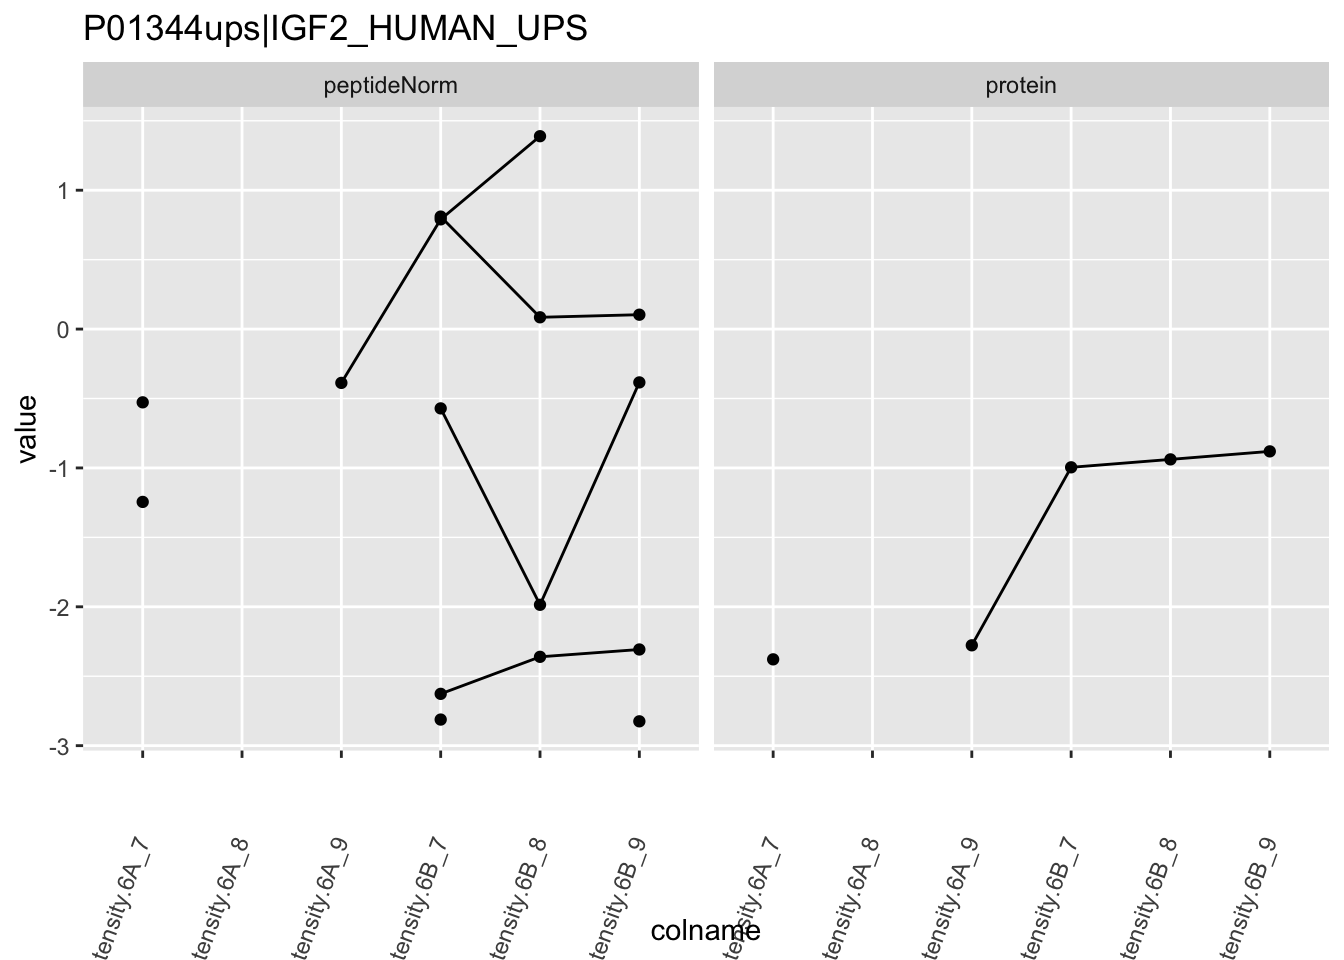
\includegraphics{sequencing_rnaseqIntro_files/figure-beamer/unnamed-chunk-21-9.pdf}
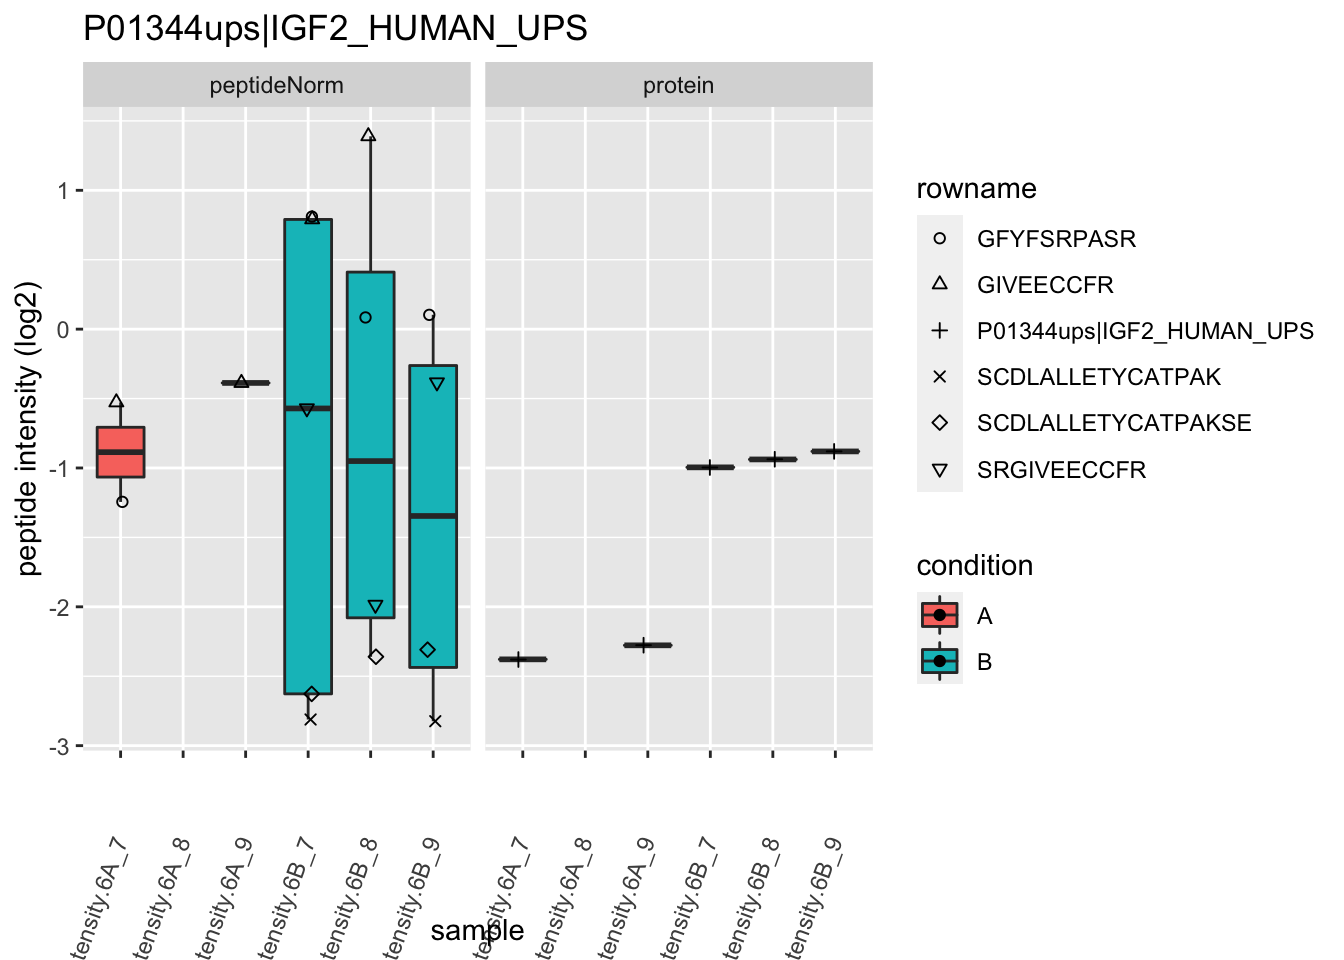
\includegraphics{sequencing_rnaseqIntro_files/figure-beamer/unnamed-chunk-21-10.pdf}
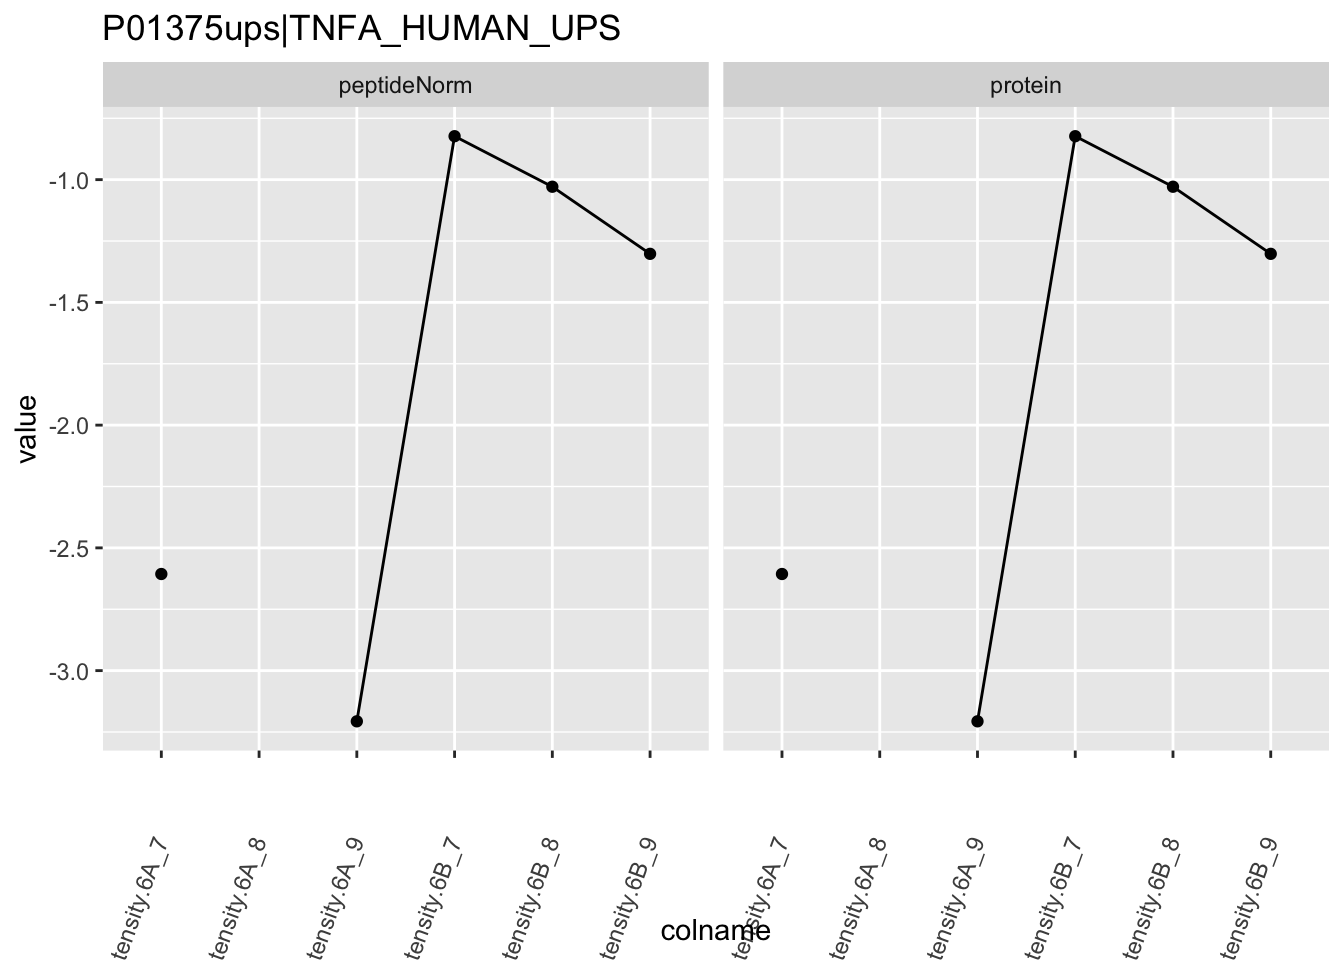
\includegraphics{sequencing_rnaseqIntro_files/figure-beamer/unnamed-chunk-21-11.pdf}
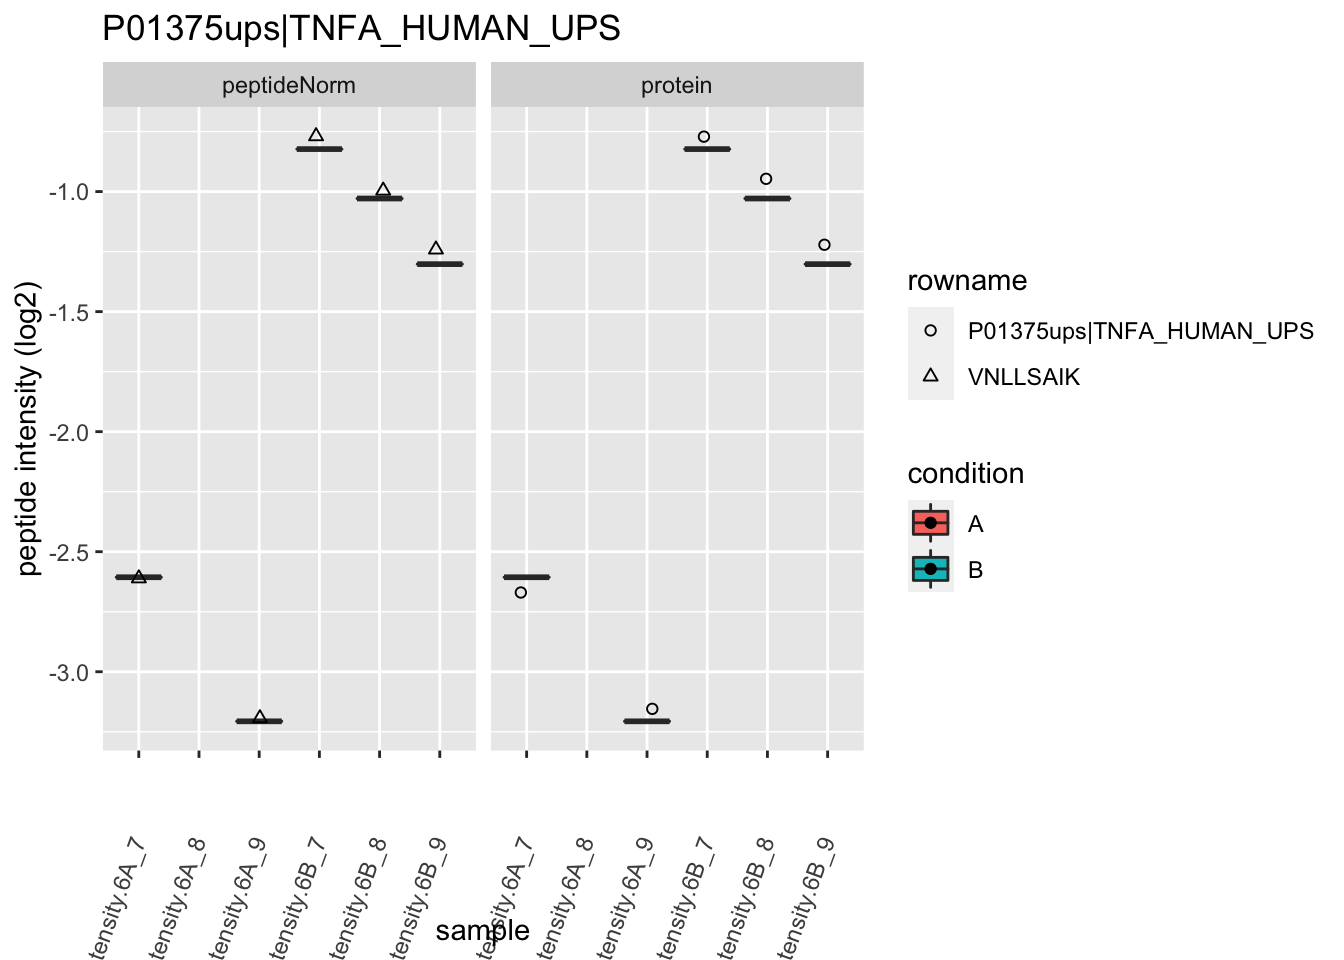
\includegraphics{sequencing_rnaseqIntro_files/figure-beamer/unnamed-chunk-21-12.pdf}
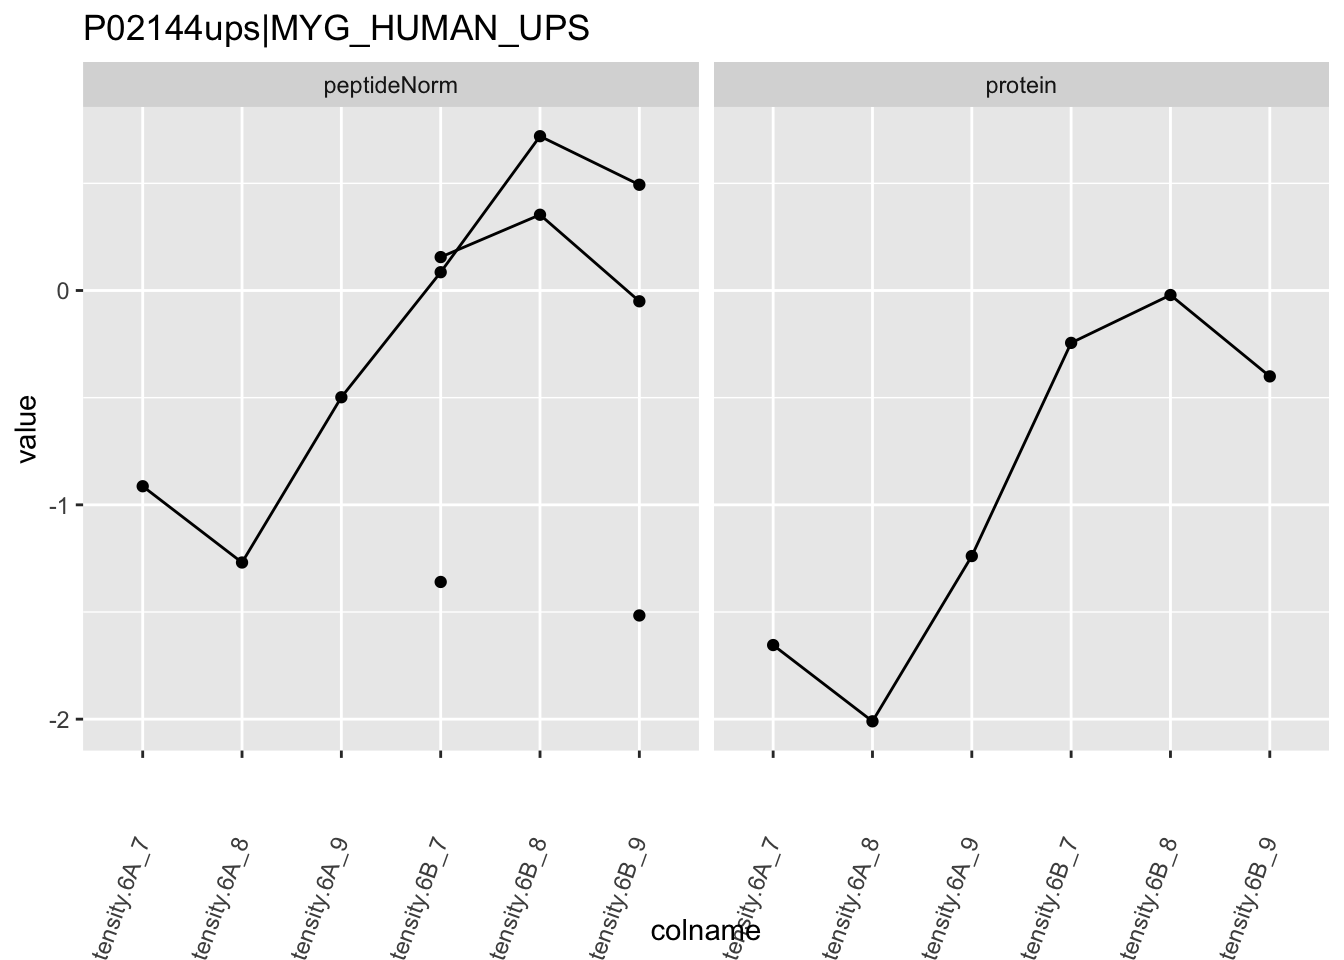
\includegraphics{sequencing_rnaseqIntro_files/figure-beamer/unnamed-chunk-21-13.pdf}
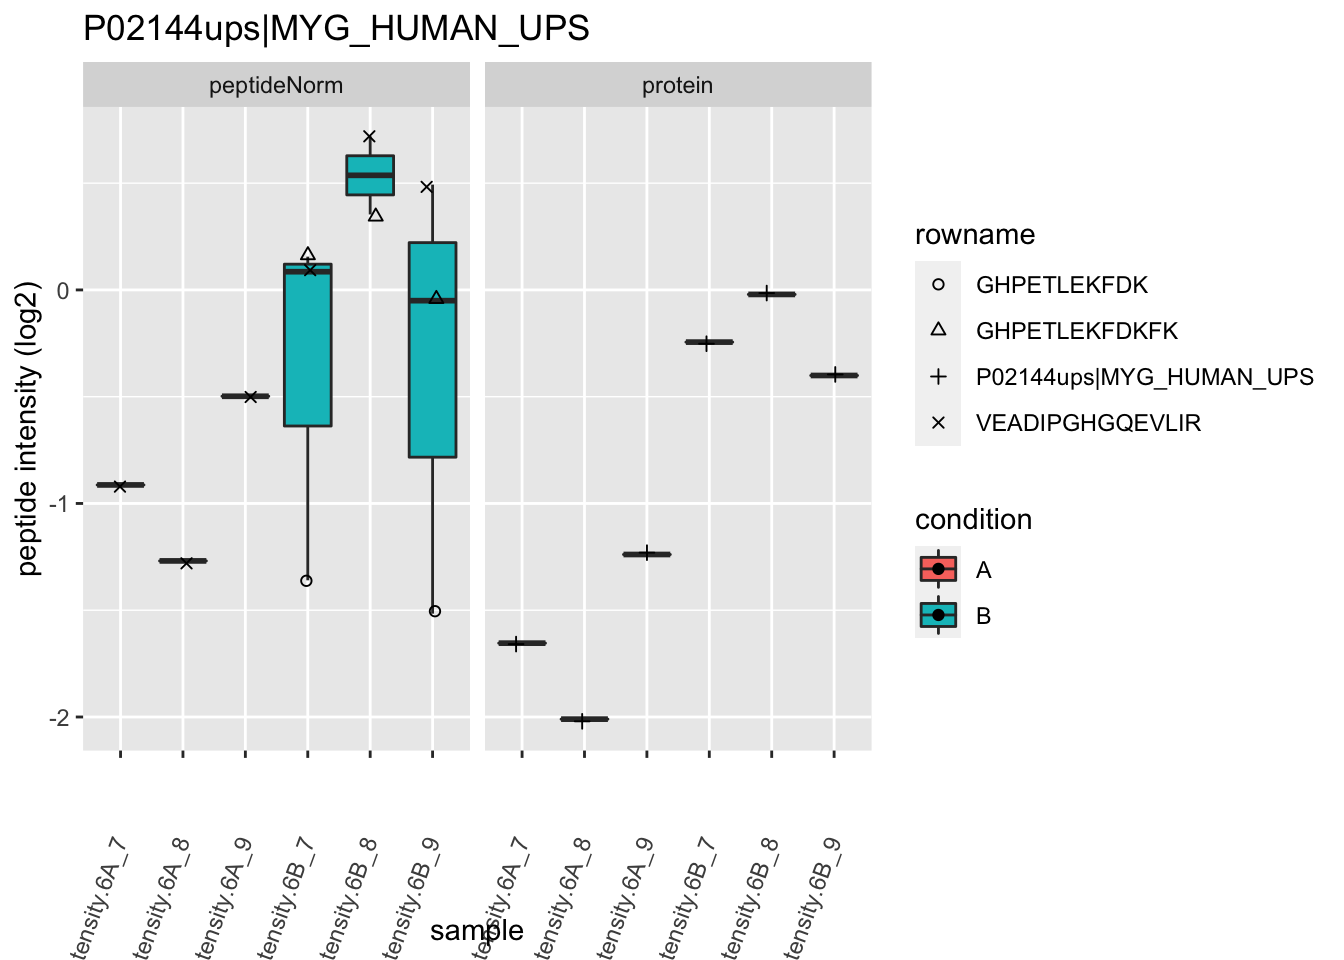
\includegraphics{sequencing_rnaseqIntro_files/figure-beamer/unnamed-chunk-21-14.pdf}
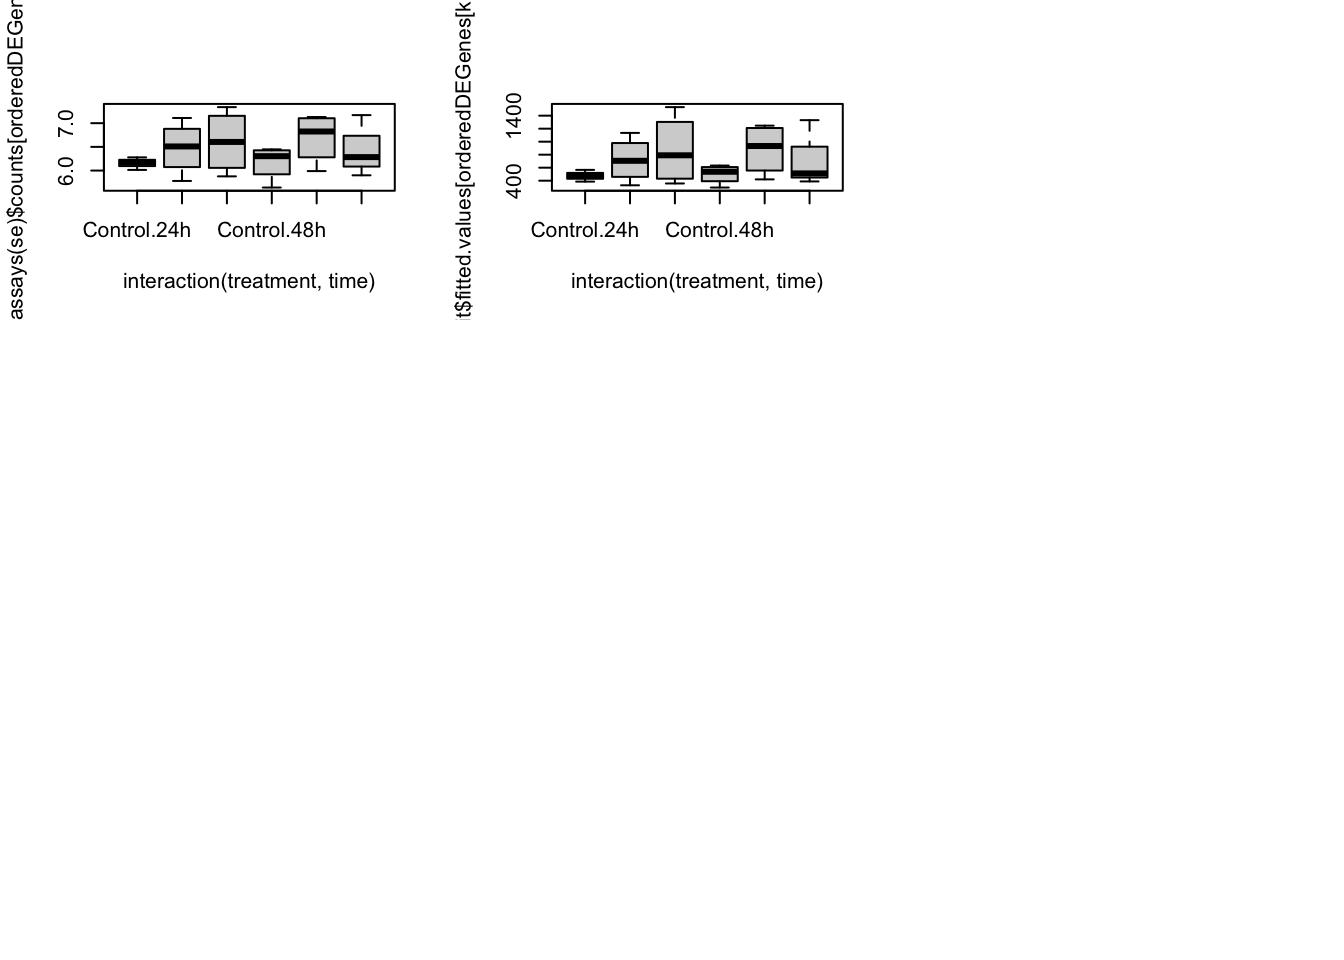
\includegraphics{sequencing_rnaseqIntro_files/figure-beamer/unnamed-chunk-21-15.pdf}

\begin{block}{Contrast on the time effect}

Based on the MDS plot, we can expect comparatively more DE genes for the
time effect. For didactic purposes, here we assess an \textbf{average
time effect across the three treatments}. The analysis shows how
flexible one can be when using contrasts.

Mean of time 24h:
\[\log \mu_{g,24h} = \frac{1}{3} \left\{ \underbrace{(\beta_{g0})}_\text{Control, 24h} + \underbrace{(\beta_{g0} + \beta_{g1})}_\text{DPN, 24h} + \underbrace{(\beta_{g0} + \beta_{g2})}_\text{OHT, 24h} \right\}\]

Mean of time 48h:
\[\log \mu_{g,48h} = \frac{1}{3} \left\{ \underbrace{(\beta_{g0} + \beta_{g3})}_\text{Control, 48h} + \underbrace{(\beta_{g0} + \beta_{g1} + \beta_{g3} + \beta_{g7})}_\text{DPN, 48h} + \underbrace{(\beta_{g0} + \beta_{g2}+ \beta_{g3} + \beta_{g8})}_\text{OHT, 48h} \right\}\]

Difference:
\[ \log \left( \frac{\mu_{g,48h}}{\mu_{g,24h}} \right) = \beta_{g3} + \frac{1}{3}(\beta_{g7} + \beta_{g8}) \]

\begin{Shaded}
\begin{Highlighting}[]
\NormalTok{Ltime <-}\StringTok{ }\KeywordTok{matrix}\NormalTok{(}\DecValTok{0}\NormalTok{, }\DataTypeTok{nrow =} \KeywordTok{ncol}\NormalTok{(fit}\OperatorTok{$}\NormalTok{coefficients), }\DataTypeTok{ncol =} \DecValTok{1}\NormalTok{)}
\KeywordTok{rownames}\NormalTok{(Ltime) <-}\StringTok{ }\KeywordTok{colnames}\NormalTok{(fit}\OperatorTok{$}\NormalTok{coefficients)}
\NormalTok{Ltime[}\KeywordTok{c}\NormalTok{(}\StringTok{"time48h"}\NormalTok{, }\StringTok{"treatmentDPN:time48h"}\NormalTok{, }\StringTok{"treatmentOHT:time48h"}\NormalTok{),}\DecValTok{1}\NormalTok{] <-}\StringTok{ }\KeywordTok{c}\NormalTok{(}\DecValTok{1}\NormalTok{, }\DecValTok{1}\OperatorTok{/}\DecValTok{3}\NormalTok{, }\DecValTok{1}\OperatorTok{/}\DecValTok{3}\NormalTok{)}

\NormalTok{lrtTime <-}\StringTok{ }\KeywordTok{glmLRT}\NormalTok{(fit, }\DataTypeTok{contrast=}\NormalTok{Ltime)}
\KeywordTok{hist}\NormalTok{(lrtTime}\OperatorTok{$}\NormalTok{table}\OperatorTok{$}\NormalTok{PValue) }\CommentTok{# very different p-value distribution}
\end{Highlighting}
\end{Shaded}

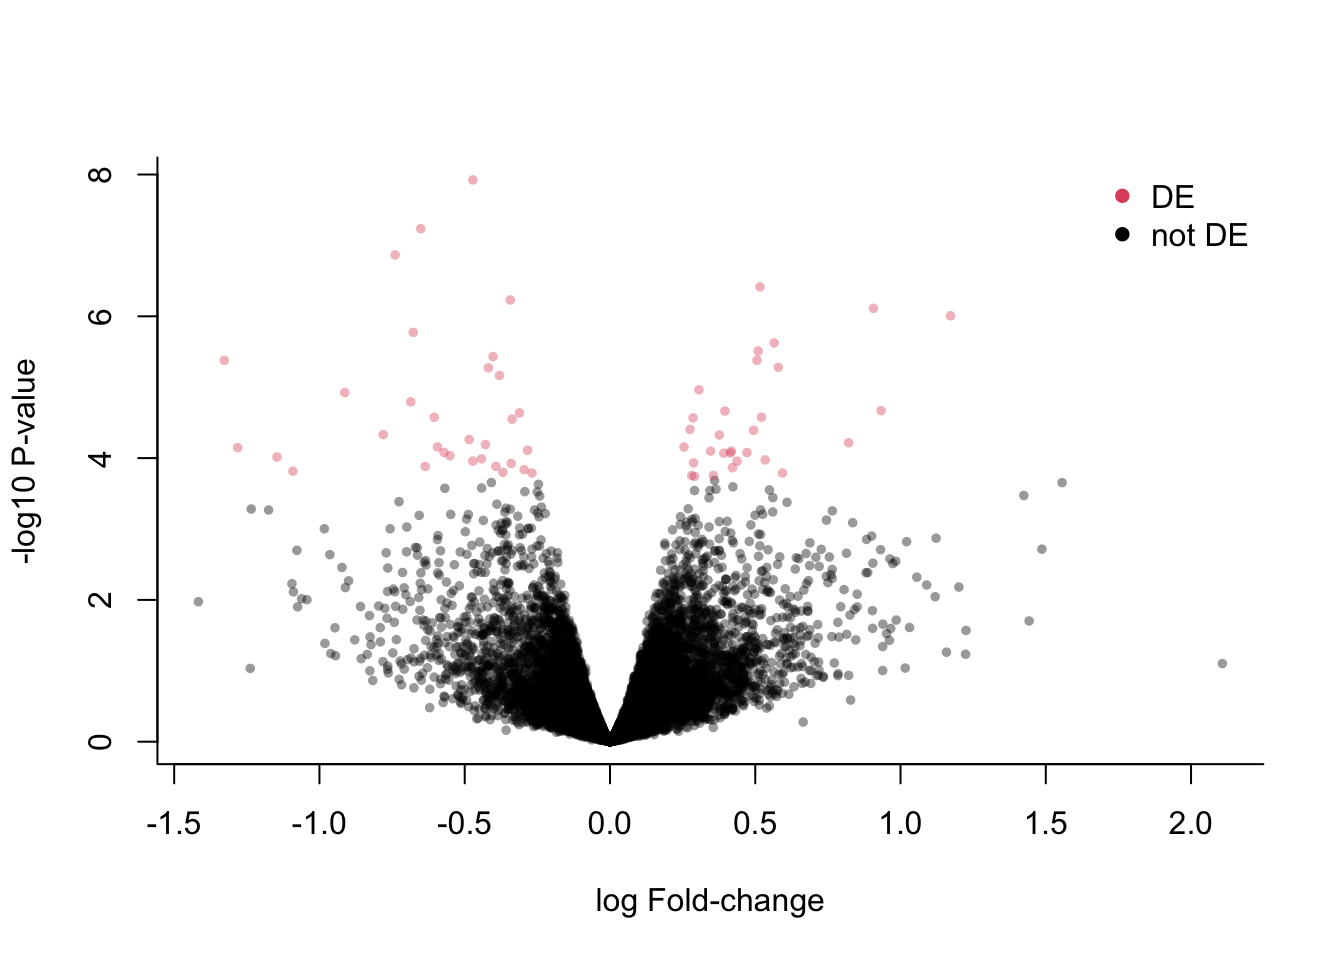
\includegraphics{sequencing_rnaseqIntro_files/figure-beamer/unnamed-chunk-22-1.pdf}

\begin{Shaded}
\begin{Highlighting}[]
\KeywordTok{sum}\NormalTok{(}\KeywordTok{p.adjust}\NormalTok{(lrtTime}\OperatorTok{$}\NormalTok{table}\OperatorTok{$}\NormalTok{PValue, }\StringTok{"fdr"}\NormalTok{) }\OperatorTok{<=}\StringTok{ }\FloatTok{0.05}\NormalTok{) }\CommentTok{# many DE genes}
\end{Highlighting}
\end{Shaded}

\begin{verbatim}
## [1] 6105
\end{verbatim}

\end{block}

\end{frame}

\begin{frame}[fragile]{Alternative parameterizations}
\protect\hypertarget{alternative-parameterizations}{}

While our design matrix here was parameterized as
\texttt{\textasciitilde{}\ treatment*time\ +\ patient} alternative,
equivalent parameterizations are also possible. Below, we demonstrate
another parameterization that could work, too, and can be more
intuitive. In this parameterization, we estimate a mean for each
experimental condition, without an intercept, which can be convenient to
think about how to set up contrasts.

\begin{Shaded}
\begin{Highlighting}[]
\NormalTok{treatTime <-}\StringTok{ }\KeywordTok{as.factor}\NormalTok{(}\KeywordTok{paste0}\NormalTok{(treatment, time))}
\KeywordTok{table}\NormalTok{(treatTime)}
\end{Highlighting}
\end{Shaded}

\begin{verbatim}
## treatTime
## Control24h Control48h     DPN24h     DPN48h     OHT24h     OHT48h 
##          3          4          4          4          4          4
\end{verbatim}

\begin{Shaded}
\begin{Highlighting}[]
\NormalTok{design2 <-}\StringTok{ }\KeywordTok{model.matrix}\NormalTok{(}\OperatorTok{~}\StringTok{ }\DecValTok{0} \OperatorTok{+}\StringTok{ }\NormalTok{treatTime }\OperatorTok{+}\StringTok{ }\NormalTok{patient)}

\NormalTok{dge2 <-}\StringTok{ }\KeywordTok{calcNormFactors}\NormalTok{(se)}
\NormalTok{dge2 <-}\StringTok{ }\KeywordTok{estimateDisp}\NormalTok{(dge2, design2)}
\KeywordTok{plotBCV}\NormalTok{(dge2)}
\end{Highlighting}
\end{Shaded}

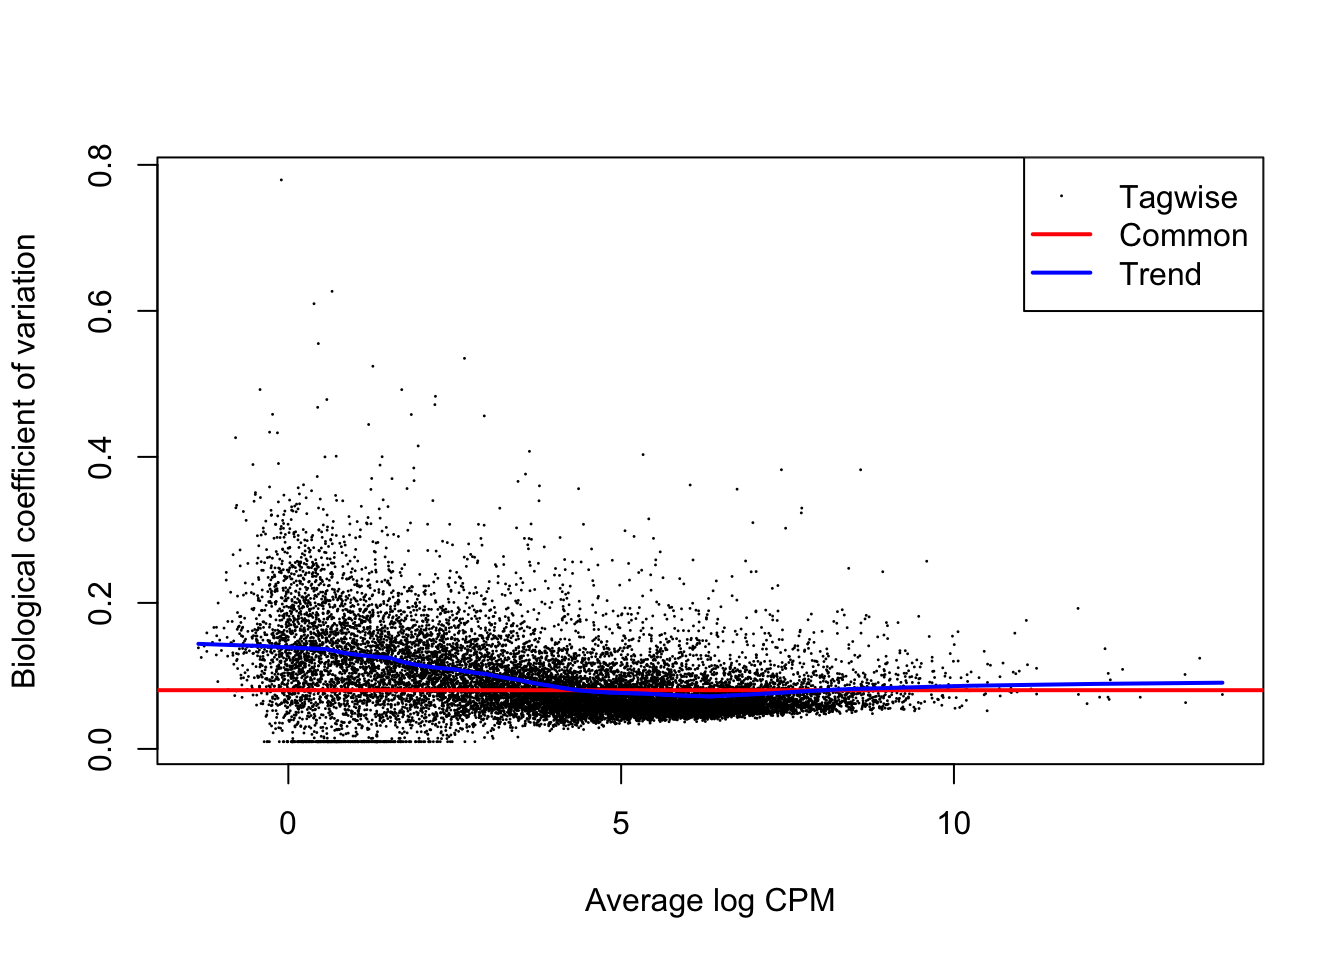
\includegraphics{sequencing_rnaseqIntro_files/figure-beamer/unnamed-chunk-23-1.pdf}

\begin{Shaded}
\begin{Highlighting}[]
\NormalTok{fit2 <-}\StringTok{ }\KeywordTok{glmFit}\NormalTok{(dge2, design2)}
\KeywordTok{head}\NormalTok{(fit2}\OperatorTok{$}\NormalTok{coefficients)}
\end{Highlighting}
\end{Shaded}

\begin{verbatim}
##                 treatTimeControl24h treatTimeControl48h treatTimeDPN24h
## ENSG00000000003           -9.331882           -9.200708       -9.220647
## ENSG00000000419          -10.373781          -10.468552      -10.426939
## ENSG00000000457          -10.934527          -11.009826      -11.063152
## ENSG00000000460          -10.097504          -10.992821      -10.009852
## ENSG00000000938          -14.696298          -14.356171      -14.675638
## ENSG00000000971          -13.686862          -13.197712      -13.394543
##                 treatTimeDPN48h treatTimeOHT24h treatTimeOHT48h   patient2
## ENSG00000000003       -9.211298       -9.246413        -9.23356 -0.5174796
## ENSG00000000419      -10.472552      -10.409628       -10.38765  0.1387269
## ENSG00000000457      -11.073841      -11.068766       -11.01182  0.4584629
## ENSG00000000460      -10.745004       -9.960816       -10.67321  0.5419252
## ENSG00000000938      -14.459554      -14.780184       -14.64988  1.4483041
## ENSG00000000971      -13.508326      -13.421332       -13.64584 -0.1460052
##                    patient3   patient4
## ENSG00000000003 -0.83223188 -0.6265133
## ENSG00000000419  0.10284160  0.1003775
## ENSG00000000457 -0.05968439  0.2070947
## ENSG00000000460 -0.33688177 -0.1340312
## ENSG00000000938  0.53981205  0.8188658
## ENSG00000000971  0.93631262 -0.2692062
\end{verbatim}

\begin{Shaded}
\begin{Highlighting}[]
\CommentTok{## for example: the estimate for the DPN24h vs control 24h is still the same,}
\CommentTok{## but requires a different combination of parameters}
\KeywordTok{plot}\NormalTok{(fit}\OperatorTok{$}\NormalTok{coefficients[,}\StringTok{"treatmentDPN"}\NormalTok{], }
\NormalTok{     fit2}\OperatorTok{$}\NormalTok{coefficients[,}\StringTok{"treatTimeDPN24h"}\NormalTok{] }\OperatorTok{-}\StringTok{ }\NormalTok{fit2}\OperatorTok{$}\NormalTok{coefficients[,}\StringTok{"treatTimeControl24h"}\NormalTok{])}
\end{Highlighting}
\end{Shaded}

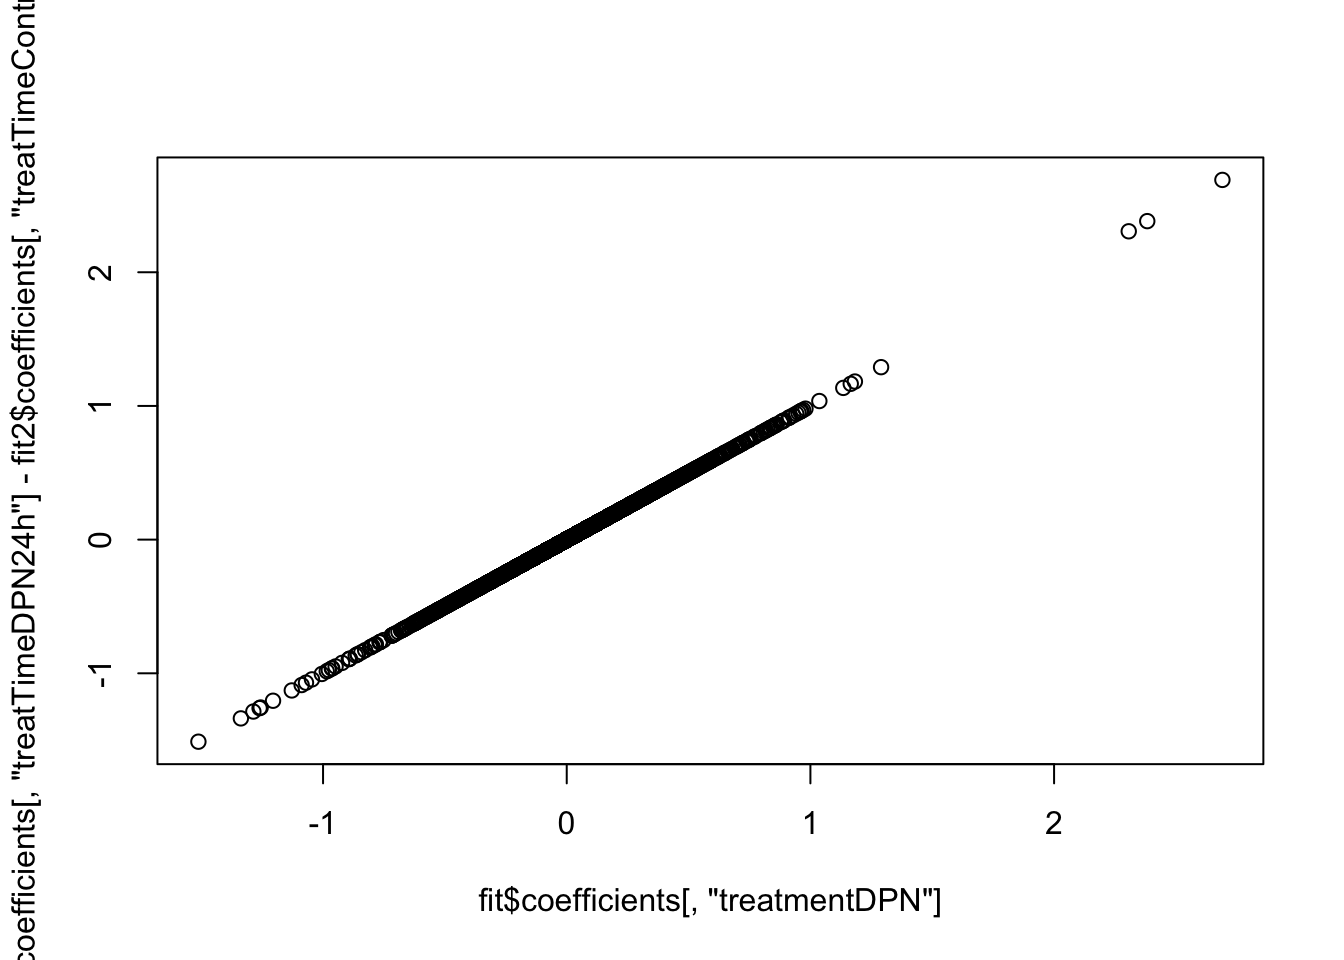
\includegraphics{sequencing_rnaseqIntro_files/figure-beamer/unnamed-chunk-23-2.pdf}

\begin{Shaded}
\begin{Highlighting}[]
\CommentTok{# Let's implement the DPNvsCON48 contrast}
\NormalTok{L2 <-}\StringTok{ }\KeywordTok{matrix}\NormalTok{(}\DecValTok{0}\NormalTok{, }\DataTypeTok{nrow =} \KeywordTok{ncol}\NormalTok{(fit2}\OperatorTok{$}\NormalTok{coefficients), }\DataTypeTok{ncol =} \DecValTok{1}\NormalTok{)}
\KeywordTok{rownames}\NormalTok{(L2) <-}\StringTok{ }\KeywordTok{colnames}\NormalTok{(fit2}\OperatorTok{$}\NormalTok{coefficients)}
\NormalTok{L2[}\KeywordTok{c}\NormalTok{(}\StringTok{"treatTimeDPN48h"}\NormalTok{, }\StringTok{"treatTimeControl48h"}\NormalTok{),}\DecValTok{1}\NormalTok{] <-}\StringTok{ }\KeywordTok{c}\NormalTok{(}\DecValTok{1}\NormalTok{, }\DecValTok{-1}\NormalTok{)}
\NormalTok{lrt2 <-}\StringTok{ }\KeywordTok{glmLRT}\NormalTok{(fit2, }\DataTypeTok{contrast=}\NormalTok{L2[,}\DecValTok{1}\NormalTok{])}
\KeywordTok{hist}\NormalTok{(lrt2}\OperatorTok{$}\NormalTok{table}\OperatorTok{$}\NormalTok{PValue)}
\end{Highlighting}
\end{Shaded}

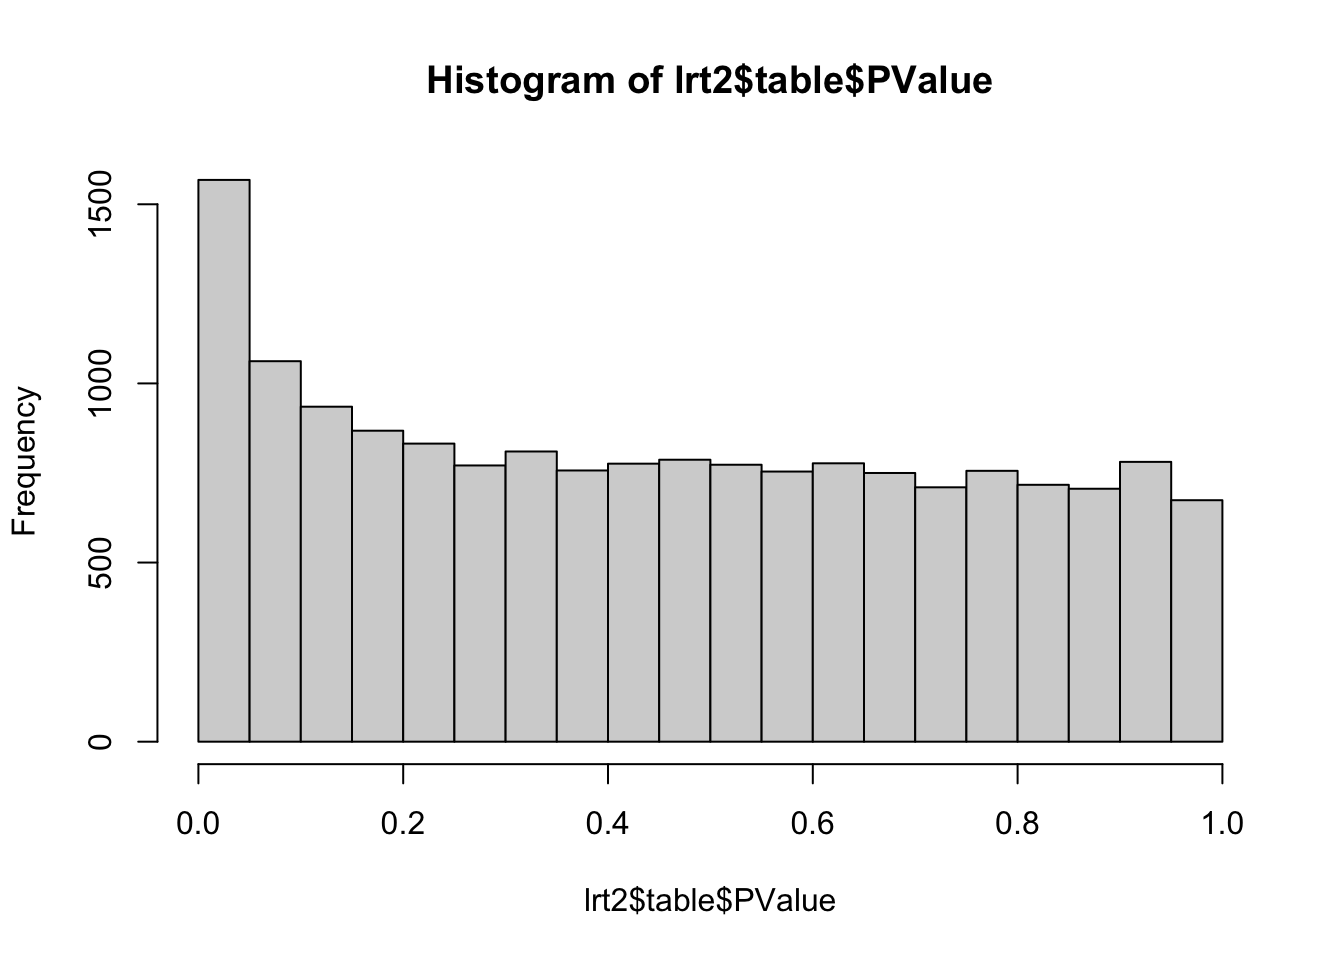
\includegraphics{sequencing_rnaseqIntro_files/figure-beamer/unnamed-chunk-23-3.pdf}

\begin{Shaded}
\begin{Highlighting}[]
\KeywordTok{plot}\NormalTok{(}\DataTypeTok{x=}\NormalTok{lrt2}\OperatorTok{$}\NormalTok{table}\OperatorTok{$}\NormalTok{PValue, }\DataTypeTok{y=}\NormalTok{lrtList[[}\DecValTok{2}\NormalTok{]]}\OperatorTok{$}\NormalTok{table}\OperatorTok{$}\NormalTok{PValue)}
\end{Highlighting}
\end{Shaded}

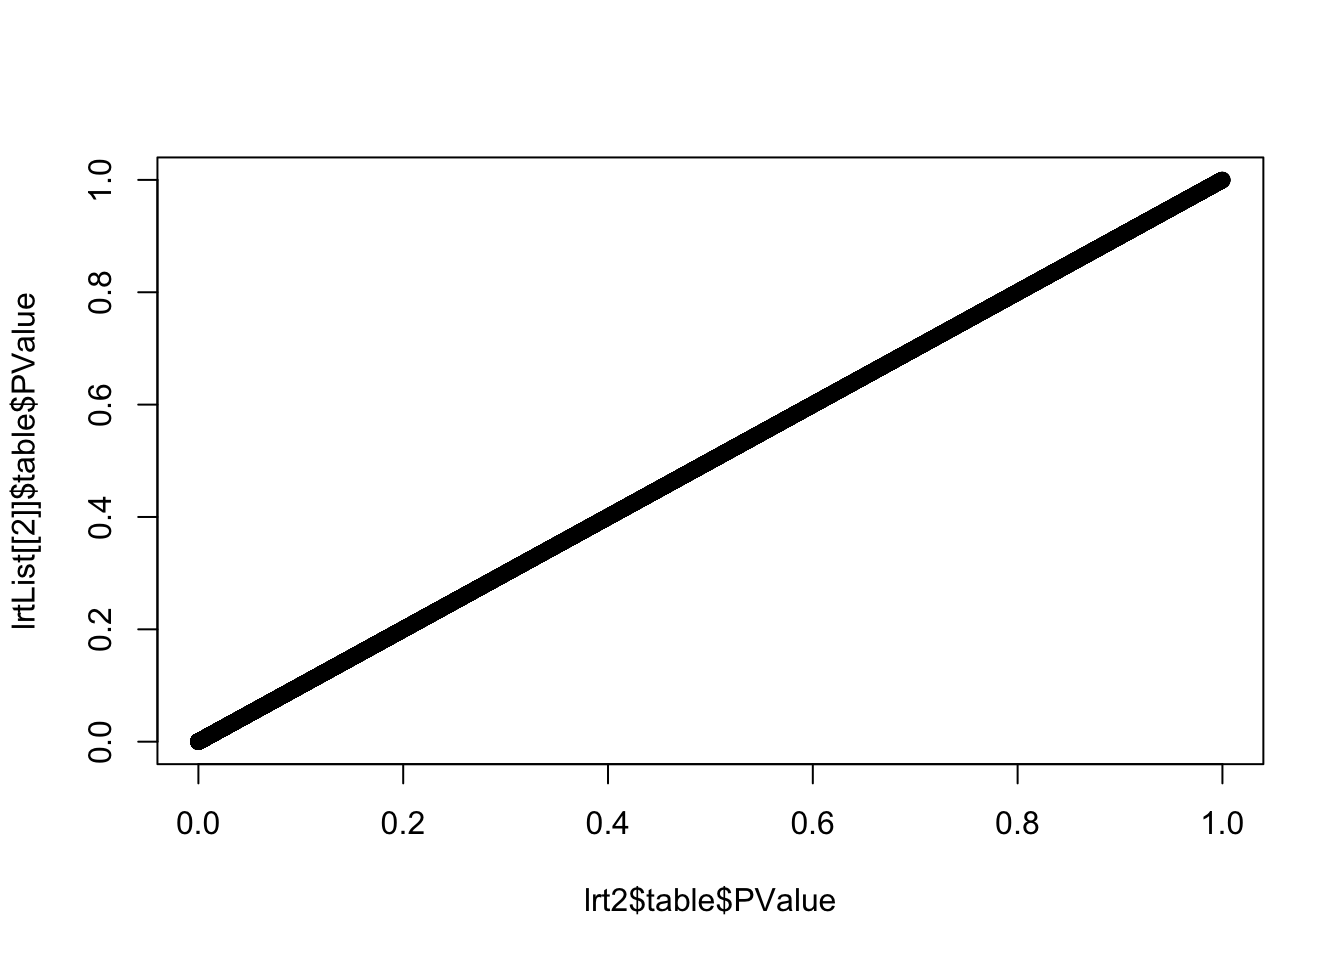
\includegraphics{sequencing_rnaseqIntro_files/figure-beamer/unnamed-chunk-23-4.pdf}

\end{frame}

\begin{frame}{Additional Challenge (Opportunity?): The importance of
reproducible analysis}
\protect\hypertarget{additional-challenge-opportunity-the-importance-of-reproducible-analysis}{}

Finally, it is crucial to make your analysis reproducible using tools
such as RMarkdown and GitHub. Please sit back and watch this
\href{https://www.youtube.com/watch?v=8QJfNS7XXwA}{amazing lecture from
Professor Keith Baggerly on "The Importance of Reproducible Research in
High-Throughput Biology}.

\end{frame}

\end{document}
